\documentclass[aspectratio=169,12pt]{beamer}
\usepackage[utf8]{inputenc}
\usepackage[T5]{fontenc}
\usepackage[vietnamese]{babel}
\usepackage{lmodern}
\usepackage{graphicx}
\usepackage{booktabs}
\usepackage{tabularx}
\usepackage{multicol}
\usepackage{tikz}
\usepackage{xcolor}

\usetheme{Madrid}
\usefonttheme{professionalfonts}

% --- Custom Colors & Settings ---
\definecolor{UBrandBlue}{RGB}{0, 71, 155}
\definecolor{UBrandGold}{RGB}{255, 184, 28}
\setbeamercolor{palette primary}{bg=UBrandBlue,fg=white}
\setbeamercolor{palette secondary}{bg=UBrandGold,fg=black}
\setbeamercolor{palette tertiary}{bg=UBrandBlue!80!black,fg=white}
\setbeamercolor{title}{bg=UBrandBlue,fg=white}
\setbeamercolor{item}{fg=UBrandBlue}


\title[Thực hành - Chương 04]{Lập Kế hoạch Dữ liệu và Chiến lược Phân tích}
\subtitle{Planning Data and Analysis Strategies}
\author[Giảng viên]{Trí tuệ Nhân tạo cho Kế toán (AI in Accounting)}
\institute[Đại học]{Khoa Kế toán - Kiểm toán}
\date{Bài giảng Thực hành 04}

\begin{document}

\begin{frame}
    \titlepage
\end{frame}

\begin{frame}{Góc nhìn Chuyên gia (Professional Insight)}
\begin{itemize}
    \item \textbf{Tại sao phải lập kế hoạch?} Một dự án phân tích dữ liệu thất bại thường không phải do thiếu công cụ hay kỹ thuật, mà do sự yếu kém trong khâu lập kế hoạch ban đầu.
    \item \textbf{Cầu nối kinh doanh và kỹ thuật:} Lập kế hoạch giúp chuyển hóa các mục tiêu kinh doanh trừu tượng thành các chỉ số kỹ thuật và chiến lược dữ liệu cụ thể.
    \item \textbf{Tiết kiệm chi phí và thời gian:} Việc phát hiện dữ liệu thiếu hoặc không đáng tin cậy ở giai đoạn lập kế hoạch rẻ hơn rất nhiều so với khi dự án đã đi vào triển khai.
\end{itemize}
\end{frame}

\begin{frame}{Lộ trình Chương (Chapter Roadmap)}
\begin{itemize}
    \item \textbf{LO 4.1:} Các thành phần của Kế hoạch Dự án Phân tích Dữ liệu.
    \item \textbf{LO 4.2:} Phát triển Chiến lược Dữ liệu (Xác định nguồn và chất lượng).
    \item \textbf{LO 4.3:} Thiết kế Chiến lược Phân tích (Áp dụng các kỹ thuật phân tích).
    \item \textbf{LO 4.4:} Chiến lược Phân tích và Dữ liệu trong Thực tiễn nghề nghiệp.
\end{itemize}
\end{frame}

\begin{frame}{4.1 Kế toán viên thiết kế dự án phân tích dữ liệu như thế nào?}
\begin{itemize}
    \item \textbf{Vai trò của Kế toán viên:} Không chỉ là người cung cấp số liệu, kế toán viên hiện đại (Business Partner) cần dẫn dắt các dự án phân tích dữ liệu để giải quyết bài toán của doanh nghiệp.
    \item \textbf{Yêu cầu của dự án thành công:} Một dự án phân tích dữ liệu cần có sự nhất quán (alignment) từ mục tiêu chiến lược, tính khả thi của dữ liệu, đến phương pháp luận thống kê phù hợp.
    \item \textbf{Cách tiếp cận có cấu trúc:} Để tránh "Rác vào - Rác ra" (Garbage in - Garbage out), việc thiết kế dự án cần tuân theo một quy trình 4 bước chặt chẽ.
\end{itemize}
\end{frame}

\begin{frame}{4 Bước tạo Kế hoạch Dự án Phân tích}

    \begin{columns}
        \begin{column}{0.45\textwidth}
\begin{itemize}
    \item \textbf{Bước 1: Mục tiêu (Objective)} - Trả lời câu hỏi "Chúng ta muốn đạt được điều gì?".
    \item \textbf{Bước 2: Chiến lược Dữ liệu (Data Strategy)} - Trả lời câu hỏi "Chúng ta cần dữ liệu gì và lấy ở đâu?".
    \item \textbf{Bước 3: Chiến lược Phân tích (Analysis Strategy)} - Trả lời câu hỏi "Làm thế nào để xử lý số dữ liệu đó?".
    \item \textbf{Bước 4: Rủi ro (Risks)} - Trả lời câu hỏi "Những rào cản nào có thể khiến dự án thất bại và cách khắc phục?".
\end{itemize}
        \end{column}
        \begin{column}{0.55\textwidth}
            \begin{figure}[h]
                \centering
                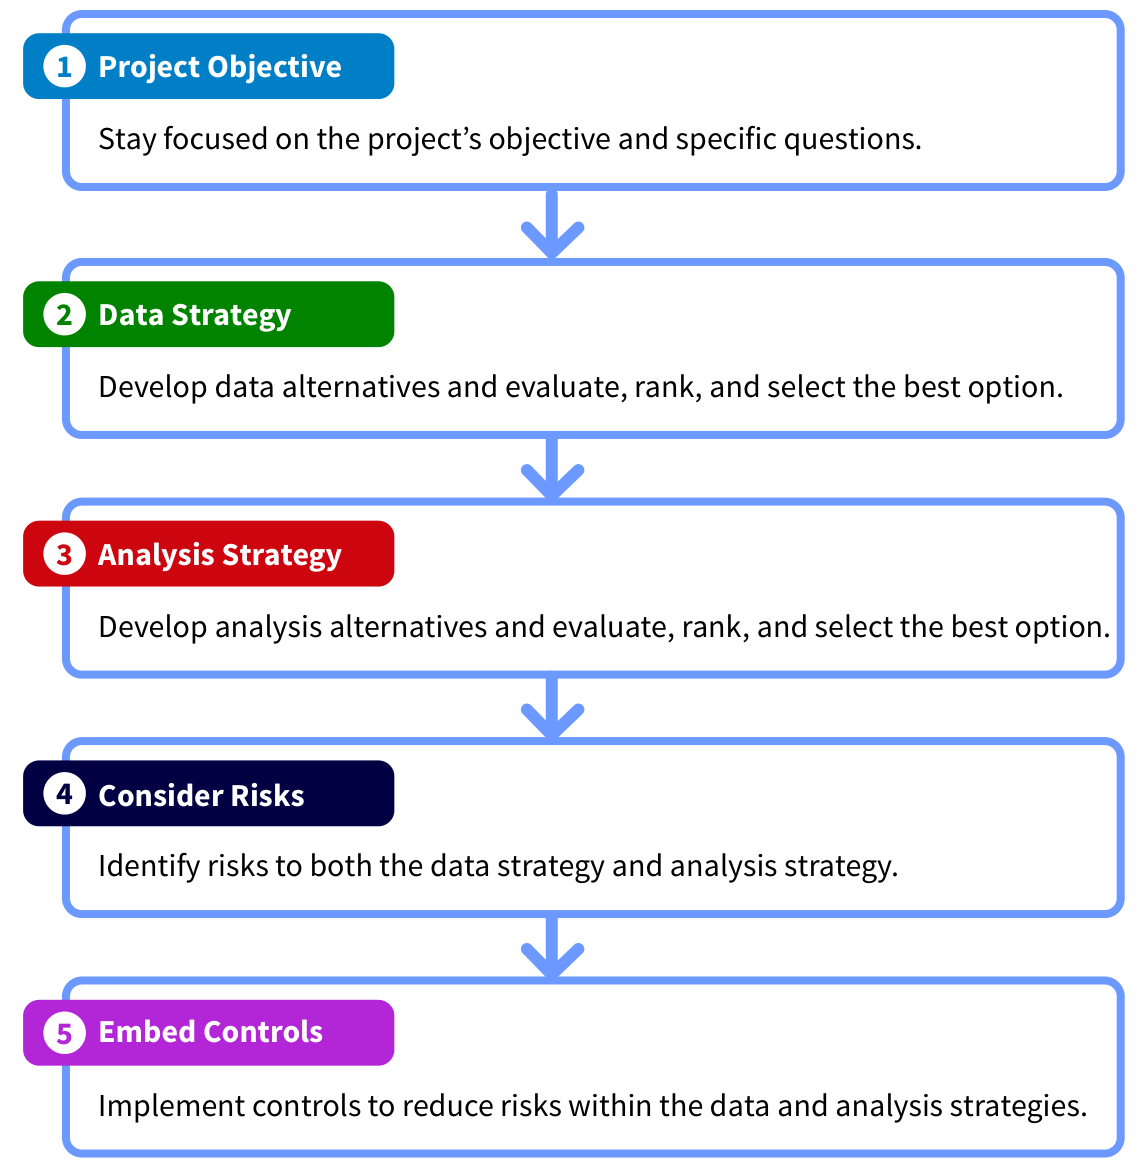
\includegraphics[width=\textwidth,height=0.75\textheight,keepaspectratio]{../textbookForPractice/Figures/Ch_04/ILLUSTRATION 4.1.png}
            \end{figure}
        \end{column}
    \end{columns}
\end{frame}

\begin{frame}{Bước 1: Tập trung vào Mục tiêu (Focus on the objective)}
\begin{itemize}
    \item \textbf{Nguồn gốc của mục tiêu:} Dựa vào Động lực (Motivations) đã được xác định từ Chương 3.
    \item \textbf{Thu hẹp phạm vi (Scoping):} Một dự án không thể trả lời mọi câu hỏi. Kế toán viên cần xác định rõ phạm vi ưu tiên để dự án khả thi.
    \item \textbf{Tiêu chí thành công (Success Criteria):} Dự án sẽ được đánh giá là thành công khi nào? (Ví dụ: Giảm 5\% sai sót trong ghi nhận doanh thu).
\end{itemize}
\end{frame}

\begin{frame}{Bước 2 \& 3: Chọn Chiến lược Dữ liệu \& Phân tích}
\begin{itemize}
    \item \textbf{Sự phụ thuộc lẫn nhau:} Chiến lược phân tích (bước 3) phụ thuộc rất lớn vào chiến lược dữ liệu (bước 2). Không thể chạy mô hình Học máy (Machine Learning) nếu chỉ có 100 dòng dữ liệu Excel.
    \item \textbf{Phù hợp với nguồn lực:} Việc lựa chọn mô hình thống kê cần dựa trên năng lực của đội ngũ, thời gian cho phép và sức mạnh hệ thống CNTT hiện có.
    \item \textbf{Ví dụ:} Nếu mục tiêu là Phát hiện gian lận thẻ tín dụng $\rightarrow$ Dữ liệu cần có là lịch sử giao dịch (Bước 2) $\rightarrow$ Chiến lược phân tích là dùng Mô hình Cây quyết định (Decision Tree - Bước 3).
\end{itemize}
\end{frame}

\begin{frame}{Bước 4: Xem xét Rủi ro (Consider risks)}
\begin{itemize}
    \item \textbf{Rủi ro dữ liệu (Data Risks):} Dữ liệu bị thiếu (Missing values), bị sai (Inaccurate), hoặc không thể kết nối các hệ thống khác nhau (Siloed data).
    \item \textbf{Rủi ro quy định (Compliance Risks):} Vi phạm quy định về bảo mật dữ liệu (như GDPR) khi phân tích thông tin cá nhân của khách hàng.
    \item \textbf{Kế hoạch dự phòng (Contingency Plan):} Đưa ra phương án giải quyết (Mitigation) nếu các rủi ro này xảy ra. (Ví dụ: Nếu không truy cập được dữ liệu trực tiếp từ ERP, sẽ dùng bản backup cuối ngày).
\end{itemize}
\end{frame}

\begin{frame}{4.2 Phát triển Chiến lược Dữ liệu (Data Strategy)}
\begin{itemize}
    \item \textbf{Định nghĩa Chiến lược Dữ liệu:} Là một kế hoạch tổng thể về cách thu thập, lưu trữ, quản lý, và bảo mật dữ liệu để phục vụ cho các mục tiêu phân tích.
    \item \textbf{Tâm điểm của Phân tích:} Dữ liệu là 'nguyên liệu thô'. Chiến lược dữ liệu đảm bảo 'nguyên liệu' này là nguyên chất và sẵn sàng để 'chế biến'.
    \item \textbf{Câu hỏi trọng tâm:} Dữ liệu nào cần thiết? Lấy từ đâu? Và làm sao biết dữ liệu đó đáng tin cậy?
\end{itemize}
\end{frame}

\begin{frame}{Xác định dữ liệu phù hợp (Identify Appropriate Data)}
\begin{itemize}
    \item \textbf{Sự liên quan (Relevance):} Dữ liệu phải có khả năng trả lời trực tiếp cho câu hỏi phân tích đã đặt ra. 
    \item \textbf{Dữ liệu nội bộ vs. Dữ liệu bên ngoài:} Kết hợp dữ liệu hệ thống ERP nội bộ với dữ liệu kinh tế vĩ mô bên ngoài (tỷ giá, lãi suất) để tăng độ chính xác của phân tích dự đoán.
    \item \textbf{Chi phí vs. Lợi ích (Cost-Benefit Analysis):} Chi phí thu thập và làm sạch một bộ dữ liệu mới có xứng đáng với giá trị thông tin mà nó mang lại hay không?
\end{itemize}
\end{frame}

\begin{frame}{Đánh giá Trường dữ liệu và Nguồn dữ liệu}
\begin{itemize}
    \item \textbf{Trường dữ liệu (Data Fields/Attributes):} Xác định chính xác các cột thông tin cần thiết. (Ví dụ: Mã KH, Ngày mua, Giá trị đơn hàng).
    \item \textbf{Bảng dữ liệu (Data Tables):} Dữ liệu thường phân tán ở nhiều bảng (Ví dụ: Bảng Thông tin khách hàng, Bảng Giao dịch). Cần biết cách kết nối (Join) các bảng này.
    \item \textbf{Đánh giá Nguồn:} Hệ thống tạo ra dữ liệu có đáng tin cậy không? Dữ liệu do con người nhập thủ công (dễ sai sót) hay được ghi nhận tự động bởi hệ thống?
\end{itemize}
\end{frame}

\begin{frame}{Phân biệt Dữ liệu Cấu trúc \& Phi cấu trúc}
\begin{itemize}
    \item \textbf{Dữ liệu Cấu trúc (Structured Data):} Dữ liệu được sắp xếp gọn gàng theo hàng và cột trong cơ sở dữ liệu quan hệ (SQL) hoặc Excel. Cực kỳ dễ phân tích.
    \item \textbf{Dữ liệu Phi cấu trúc (Unstructured Data):} Dữ liệu không có định dạng chuẩn mực như email kế toán, hợp đồng dạng PDF, hình ảnh hóa đơn, hoặc bình luận của khách hàng trên mạng xã hội.
    \item \textbf{Thách thức của Kế toán 4.0:} Kế toán viên cần áp dụng AI và Xử lý ngôn ngữ tự nhiên (NLP) để phân tích hơn 80\% lượng dữ liệu của doanh nghiệp vốn nằm ở dạng phi cấu trúc.
\end{itemize}
\end{frame}

\begin{frame}{Các thang đo lường dữ liệu}
\begin{itemize}
    \item \textbf{Nominal (Định danh):} Phân loại không có thứ tự (VD: Phương thức thanh toán: Tiền mặt, Thẻ tín dụng, Chuyển khoản).
    \item \textbf{Ordinal (Thứ bậc):} Phân loại có thứ tự nhưng khoảng cách không đều (VD: Đánh giá chất lượng kiểm toán: Kém, Đạt, Tốt, Xuất sắc).
    \item \textbf{Interval (Khoảng):} Khoảng cách bằng nhau nhưng không có số 0 tuyệt đối (VD: Nhiệt độ, Năm tài chính). Có thể cộng trừ nhưng không thể nhân chia.
    \item \textbf{Ratio (Tỷ lệ):} Có số 0 tuyệt đối mang ý nghĩa "không có gì" (VD: Doanh thu = 0, Hàng tồn kho = 0). Hỗ trợ mọi phép toán.
\end{itemize}
\end{frame}

\begin{frame}{Các loại Dữ liệu Kế toán: Danh mục, Trạng thái, Sự kiện}
\begin{itemize}
    \item \textbf{Dữ liệu Danh mục (Master Data):} Thông tin cốt lõi, ít thay đổi của doanh nghiệp như Danh mục Tài khoản, Danh mục Khách hàng, Danh mục Hàng hóa.
    \item \textbf{Dữ liệu Trạng thái (Reference Data):} Các bảng mã, quy định thuế, tỷ giá hối đoái.
    \item \textbf{Dữ liệu Sự kiện (Transactional Data):} Sinh ra từ các giao dịch hàng ngày (Ví dụ: Chứng từ bán hàng, Phiếu thu, Phiếu chi). Số lượng rất lớn và tăng liên tục.
\end{itemize}
\end{frame}

\begin{frame}{Các Rủi ro trong Chiến lược Dữ liệu \& Cách Kiểm soát}
\begin{itemize}
    \item \textbf{Rủi ro Trùng lặp (Duplication):} Một khách hàng tồn tại thành 2 mã khác nhau trong hệ thống.
    \item \textbf{Rủi ro Thiếu sót (Completeness):} Các trường thông tin bắt buộc bị bỏ trống.
    \item \textbf{Kiểm soát (Controls):} Áp dụng các quy tắc xác thực dữ liệu (Data Validation rules) ngay tại khâu nhập liệu trên hệ thống phần mềm.
\end{itemize}
\end{frame}

\begin{frame}{Rủi ro về Khả năng truy cập (Accessibility Risks)}

    \begin{columns}
        \begin{column}{0.45\textwidth}
\begin{itemize}
    \item \textbf{Hạn chế kỹ thuật:} Dữ liệu nằm trong các hệ thống Legacy (cũ) không hỗ trợ xuất dữ liệu ra định dạng chuẩn (CSV, API).
    \item \textbf{Hạn chế phân quyền:} Kế toán viên không được cấp quyền truy cập vào dữ liệu của bộ phận Bán hàng hoặc Nhân sự để phân tích chéo.
    \item \textbf{Giải pháp:} Xây dựng Kho dữ liệu (Data Warehouse) hoặc Hồ dữ liệu (Data Lake) tập trung và xây dựng cơ chế phân quyền rõ ràng.
\end{itemize}
        \end{column}
        \begin{column}{0.55\textwidth}
            \begin{figure}[h]
                \centering
                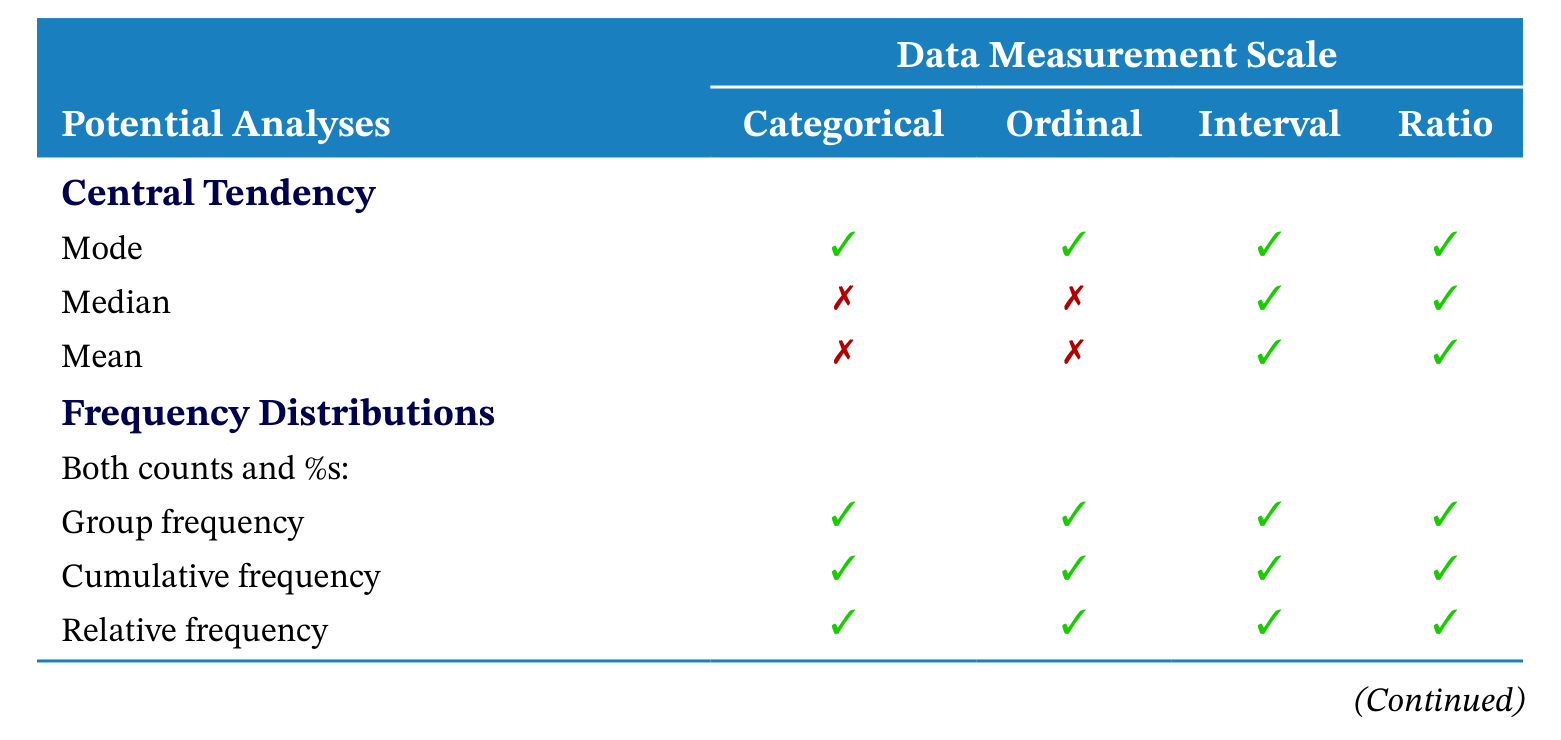
\includegraphics[width=\textwidth,height=0.75\textheight,keepaspectratio]{../textbookForPractice/Figures/Ch_04/ILLUSTRATION 4.14.png}
            \end{figure}
        \end{column}
    \end{columns}
\end{frame}

\begin{frame}{Rủi ro về Độ tin cậy và Tính toàn vẹn}
\begin{itemize}
    \item \textbf{Độ tin cậy (Reliability):} Dữ liệu có phản ánh đúng bản chất giao dịch kinh tế hay không? (Ví dụ: Doanh thu có được ghi nhận đúng kỳ?).
    \item \textbf{Tính toàn vẹn (Integrity):} Dữ liệu có bị chỉnh sửa trái phép sau khi được ghi nhận không?
    \item \textbf{Bảo vệ tính toàn vẹn:} Sử dụng công nghệ Blockchain hoặc các nhật ký hệ thống (Audit Trails) không thể tẩy xóa để theo dõi lịch sử chỉnh sửa dữ liệu.
\end{itemize}
\end{frame}

\begin{frame}{4.3 Thiết kế Chiến lược Phân tích (Analysis Strategy)}
\begin{itemize}
    \item \textbf{Lựa chọn Mô hình:} Sau khi đã có dữ liệu sạch, bước tiếp theo là chọn thuật toán/mô hình thống kê phù hợp để "nói chuyện" với dữ liệu.
    \item \textbf{Sự đánh đổi (Trade-off):} Mô hình đơn giản thì dễ giải thích nhưng độ chính xác thấp. Mô hình phức tạp (Deep Learning) có độ chính xác cao nhưng lại là "Hộp đen" (Black box) khó giải trình trước cơ quan kiểm toán.
    \item \textbf{Nguyên tắc Occam's Razor:} Ưu tiên sử dụng mô hình đơn giản nhất có thể giải quyết được mục tiêu phân tích.
\end{itemize}
\end{frame}

\begin{frame}{Thiết kế Phân tích Mô tả (Descriptive Analysis)}
\begin{itemize}
    \item \textbf{Mục tiêu:} Tóm tắt dữ liệu lịch sử một cách trực quan và dễ hiểu nhất cho Ban giám đốc.
    \item \textbf{Kỹ thuật Phân tích Ngang (Horizontal Analysis):} So sánh báo cáo tài chính qua nhiều năm để thấy xu hướng tăng/giảm.
    \item \textbf{Kỹ thuật Phân tích Dọc (Vertical Analysis):} Phân tích quy mô chung, biểu diễn các khoản mục theo tỷ lệ \% của doanh thu hoặc tổng tài sản.
    \item \textbf{Thống kê cơ bản:} Tính toán các giá trị Trung bình (Mean), Trung vị (Median), và Phương sai (Variance) để hiểu sự phân bổ của chi phí.
\end{itemize}
\end{frame}

\begin{frame}{Thiết kế Phân tích Chẩn đoán (Diagnostic Analysis)}
\begin{itemize}
    \item \textbf{Mục tiêu:} Đào sâu vào nguyên nhân của các hiện tượng đã được phát hiện trong khâu mô tả.
    \item \textbf{Phân tích Biến động (Variance Analysis):} Trong kế toán quản trị, so sánh Chi phí thực tế vs. Chi phí định mức và phân tích thành các nhân tố (Giá, Lượng).
    \item \textbf{Phân tích Benford (Benford's Law):} Trong kiểm toán, áp dụng định luật Benford để kiểm tra tần suất xuất hiện tự nhiên của các chữ số đầu tiên trong các khoản chi, nhằm khoanh vùng dấu hiệu gian lận.
    \item \textbf{Hệ số tương quan (Correlation Coefficient):} Tìm hiểu xem sự thay đổi của biến này (Chi phí Marketing) có đi kèm sự thay đổi của biến kia (Doanh thu) hay không.
\end{itemize}
\end{frame}

\begin{frame}{Thiết kế Phân tích Dự đoán (Predictive Analysis)}
\begin{itemize}
    \item \textbf{Mục tiêu:} Chuyển dữ liệu lịch sử thành dự báo tương lai thông qua các mô hình toán học và Machine Learning.
    \item \textbf{Phân tích Hồi quy (Regression Analysis):} Dùng để dự đoán chi phí hỗn hợp (hồi quy tuyến tính) hoặc dự báo xác suất phá sản (hồi quy Logistic - Altman Z-score).
    \item \textbf{Chuỗi thời gian (Time-series Forecasting):} Sử dụng thuật toán ARIMA hoặc Exponential Smoothing để dự báo doanh số bán lẻ trong các tháng tới dựa trên tính mùa vụ.
\end{itemize}
\end{frame}

\begin{frame}{Thiết kế Phân tích Đề xuất (Prescriptive Analysis)}
\begin{itemize}
    \item \textbf{Mục tiêu:} Khuyến nghị hành động tối ưu dựa trên kết quả dự đoán và các ràng buộc thực tế của doanh nghiệp.
    \item \textbf{Phân tích Dòng tiền chiết khấu (DCF):} Trong việc lập ngân sách vốn (Capital Budgeting), sử dụng NPV, IRR để quyết định có nên đầu tư vào dự án mới hay không.
    \item \textbf{Điểm ranh giới (Break-even Analysis):} Phân tích C-V-P (Chi phí - Sản lượng - Lợi nhuận) kết hợp What-if để tìm điểm hòa vốn và tối đa hóa lợi nhuận.
    \item \textbf{Quy hoạch tuyến tính (Linear Programming):} Phân bổ nguồn ngân sách giới hạn cho các chiến dịch quảng cáo sao cho tỷ lệ ROI đạt mức tối đa.
\end{itemize}
\end{frame}

\begin{frame}{4.4 Ứng dụng Chiến lược trong Thực tiễn Nghề nghiệp}
\begin{itemize}
    \item \textbf{Tính đặc thù:} Chiến lược dữ liệu và phân tích sẽ biến đổi tùy thuộc vào vị trí và trách nhiệm của kế toán viên trong tổ chức.
    \item \textbf{Yêu cầu về tư duy (Critical Thinking):} Công cụ chỉ là phương tiện. Kế toán viên cần có tư duy phản biện để đánh giá xem kết quả phân tích có hợp lý về mặt kinh tế (Economic substance) hay không.
    \item Các slide tiếp theo sẽ đi sâu vào chiến lược áp dụng cho AIS, Kiểm toán, Kế toán Tài chính, Kế toán Quản trị và Kế toán Thuế.
\end{itemize}
\end{frame}

\begin{frame}{Hệ thống Thông tin Kế toán (AIS) - Đánh giá rủi ro hệ thống}
\begin{itemize}
    \item \textbf{Chiến lược Dữ liệu:} Trích xuất Log files (Nhật ký truy cập) và Bảng Phân quyền (Access Control Lists).
    \item \textbf{Chiến lược Phân tích:} Sử dụng thuật toán phân nhóm (Clustering) để tìm ra các tài khoản user có hành vi truy cập hệ thống bất thường vào ngoài giờ hành chính.
    \item \textbf{Mục tiêu:} Tăng cường kiểm soát an ninh thông tin và ngăn ngừa gian lận từ bên trong (Internal Threats).
\end{itemize}
\end{frame}

\begin{frame}{Kiểm toán (Auditing) - Xác minh bằng chứng kiểm toán}
\begin{itemize}
    \item \textbf{Chiến lược Dữ liệu:} Sử dụng toàn bộ tệp dữ liệu Sổ cái (General Ledger) thay vì chỉ chọn mẫu ngẫu nhiên (Sampling).
    \item \textbf{Chiến lược Phân tích:} Chạy các kịch bản kiểm toán tự động (CAATs) để tìm kiếm các bút toán kép, bút toán ghi nhận vào ngày nghỉ lễ, hoặc bút toán đảo vào đầu kỳ sau.
    \item \textbf{Mục tiêu:} Nâng cao mức độ đảm bảo của bằng chứng kiểm toán và tối ưu hóa thời gian thực địa (Fieldwork).
\end{itemize}
\end{frame}

\begin{frame}{Kế toán Tài chính - Phân tích báo cáo}
\begin{itemize}
    \item \textbf{Chiến lược Dữ liệu:} Sử dụng dữ liệu báo cáo tài chính đã được chuẩn hóa theo chuẩn XBRL (eXtensible Business Reporting Language).
    \item \textbf{Chiến lược Phân tích:} Phân tích cấu trúc ngành (Industry Benchmarking) và ứng dụng Học máy để đánh giá chất lượng lợi nhuận (Earnings Quality) của doanh nghiệp so với đối thủ cạnh tranh.
    \item \textbf{Mục tiêu:} Tăng cường tính minh bạch và đánh giá khách quan sức khỏe tài chính của doanh nghiệp cho nhà đầu tư.
\end{itemize}
\end{frame}

\begin{frame}{Kế toán Quản trị - Đánh giá hiệu suất}
\begin{itemize}
    \item \textbf{Chiến lược Dữ liệu:} Tích hợp dữ liệu chi phí từ ERP với dữ liệu phi cấu trúc từ bộ cảm biến (IoT Sensors) trên dây chuyền sản xuất.
    \item \textbf{Chiến lược Phân tích:} Phân tích sự hao hụt nguyên vật liệu theo thời gian thực (Real-time tracking) để cảnh báo sớm tình trạng hỏng hóc máy móc hoặc thao tác sai của công nhân.
    \item \textbf{Mục tiêu:} Tối đa hóa hiệu quả hoạt động (Operational Efficiency) và áp dụng triệt để phương pháp chi phí mục tiêu.
\end{itemize}
\end{frame}

\begin{frame}{Kế toán Thuế - Lập kế hoạch thuế}
\begin{itemize}
    \item \textbf{Chiến lược Dữ liệu:} Thu thập dữ liệu giao dịch liên kết xuyên biên giới và quy định thuế của các quốc gia sở tại.
    \item \textbf{Chiến lược Phân tích:} Phân tích kịch bản (Scenario Analysis) để tính toán ảnh hưởng của sự thay đổi thuế suất toàn cầu (Ví dụ: Thuế tối thiểu toàn cầu) lên dòng tiền của Tập đoàn.
    \item \textbf{Mục tiêu:} Quản trị rủi ro thuế và cấu trúc các giao dịch hiệu quả để bảo vệ lợi ích hợp pháp của doanh nghiệp.
\end{itemize}
\end{frame}

\begin{frame}{Áp dụng Tư duy Phản biện (Applying Critical Thinking 4.4)}

    \begin{columns}
        \begin{column}{0.45\textwidth}
\begin{itemize}
    \item \textbf{Tình huống:} Đánh giá một kế hoạch phân tích dữ liệu do một bộ phận khác đề xuất.
    \item \textbf{Nhiệm vụ:} Sử dụng quy trình 4 bước để xem xét liệu mục tiêu, chiến lược dữ liệu và chiến lược phân tích đã thực sự "đồng điệu" (aligned) hay chưa.
    \item \textbf{Mục tiêu:} Không nhắm mắt làm theo dữ liệu, mà phải đánh giá tính hợp lý và rủi ro tiềm ẩn của các đề xuất kinh doanh.
\end{itemize}
        \end{column}
        \begin{column}{0.55\textwidth}
            \begin{figure}[h]
                \centering
                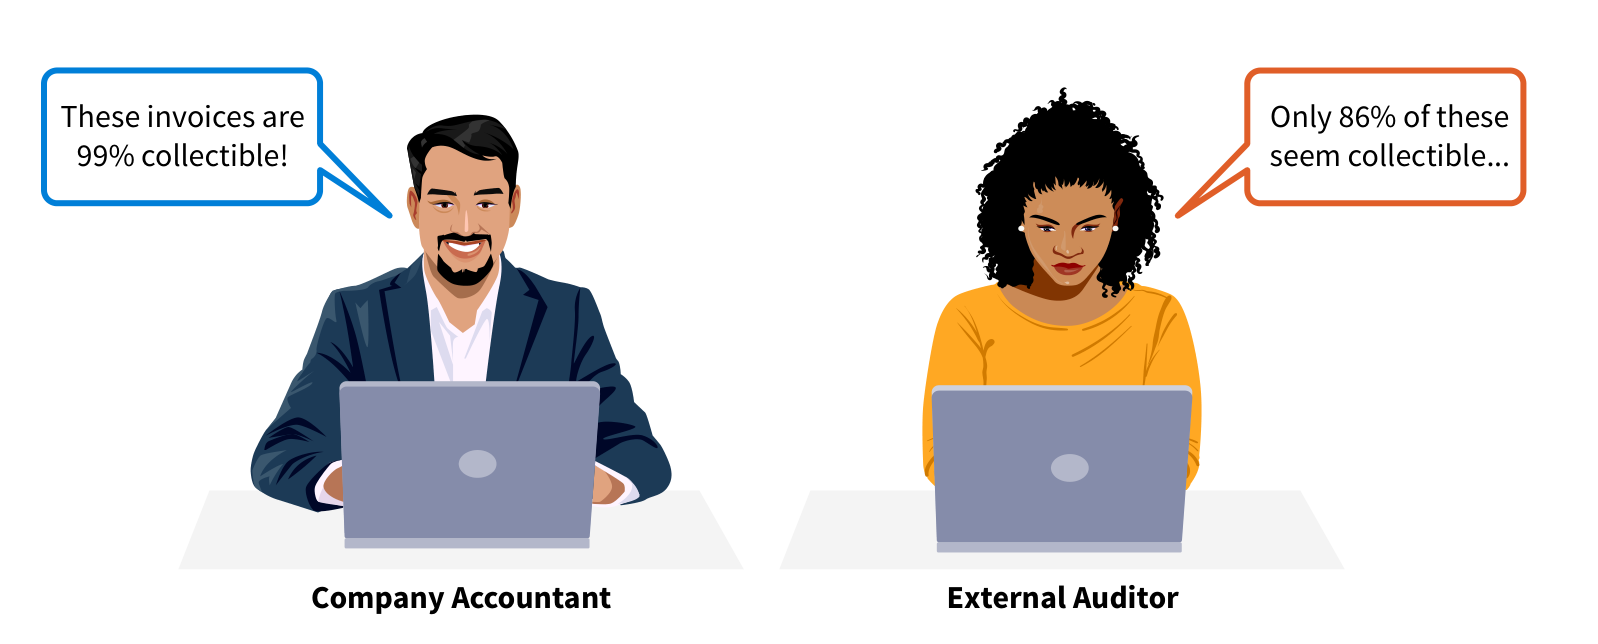
\includegraphics[width=\textwidth,height=0.75\textheight,keepaspectratio]{../textbookForPractice/Figures/Ch_04/Applying critical thinking 4.4.png}
            \end{figure}
        \end{column}
    \end{columns}
\end{frame}

\begin{frame}{Tóm tắt Mục tiêu Học tập}
\begin{itemize}
    \item \textbf{LO 4.1:} Nắm được 4 bước cốt lõi để lập kế hoạch phân tích dữ liệu: Mục tiêu, Dữ liệu, Phân tích, Rủi ro.
    \item \textbf{LO 4.2:} Phát triển chiến lược dữ liệu, phân loại được cấu trúc dữ liệu, thang đo lường và nhận diện các rủi ro về chất lượng dữ liệu.
    \item \textbf{LO 4.3:} Thiết kế chiến lược phân tích phù hợp (Mô tả, Chẩn đoán, Dự đoán, Đề xuất) để trả lời mục tiêu kinh doanh.
    \item \textbf{LO 4.4:} Ứng dụng tư duy phản biện vào các bài toán thực tiễn của Kiểm toán, AIS, Kế toán Tài chính và Kế toán Quản trị.
\end{itemize}
\end{frame}

\begin{frame}{ILLUSTRATION 4.10}
    \begin{figure}[h]
        \centering
        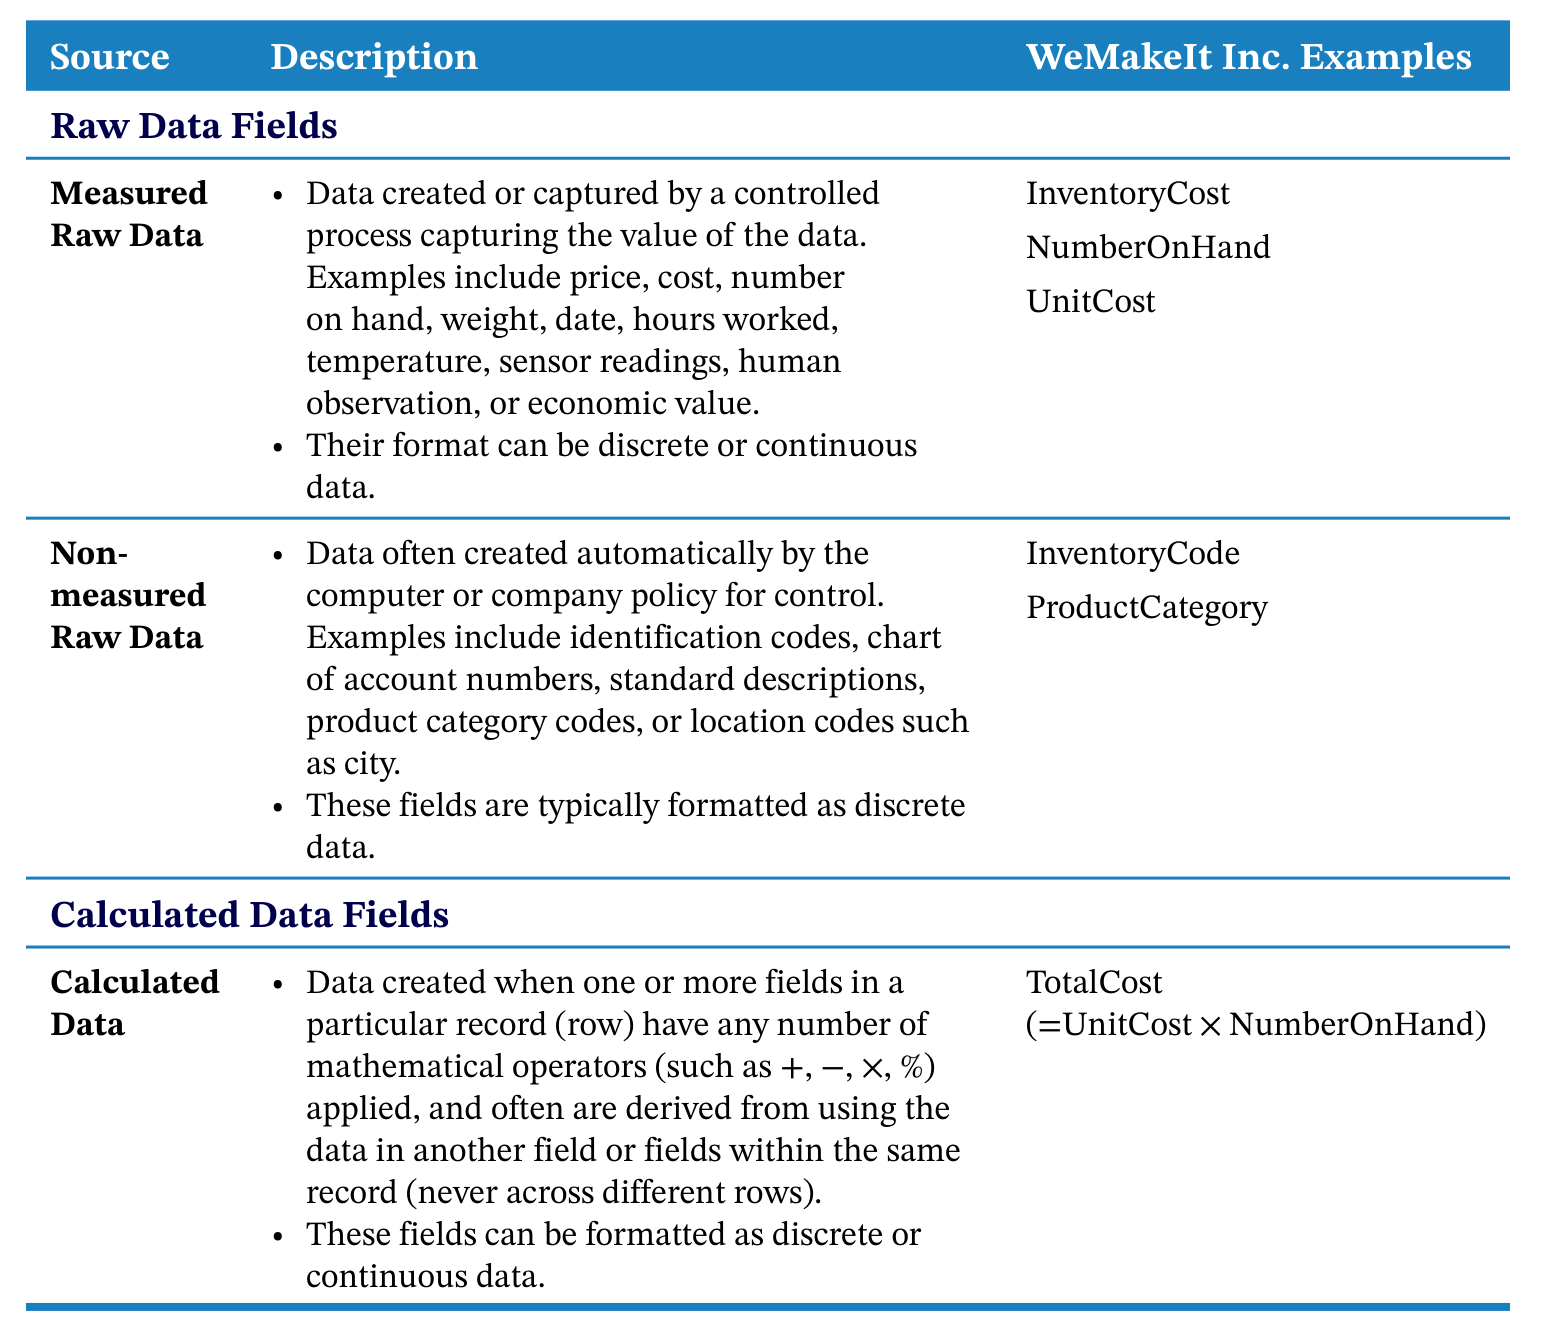
\includegraphics[width=0.95\textwidth,height=0.75\textheight,keepaspectratio]{../textbookForPractice/Figures/Ch_04/ILLUSTRATION 4.10.png}
    \end{figure}
\end{frame}

\begin{frame}{ILLUSTRATION 4.11}
    \begin{figure}[h]
        \centering
        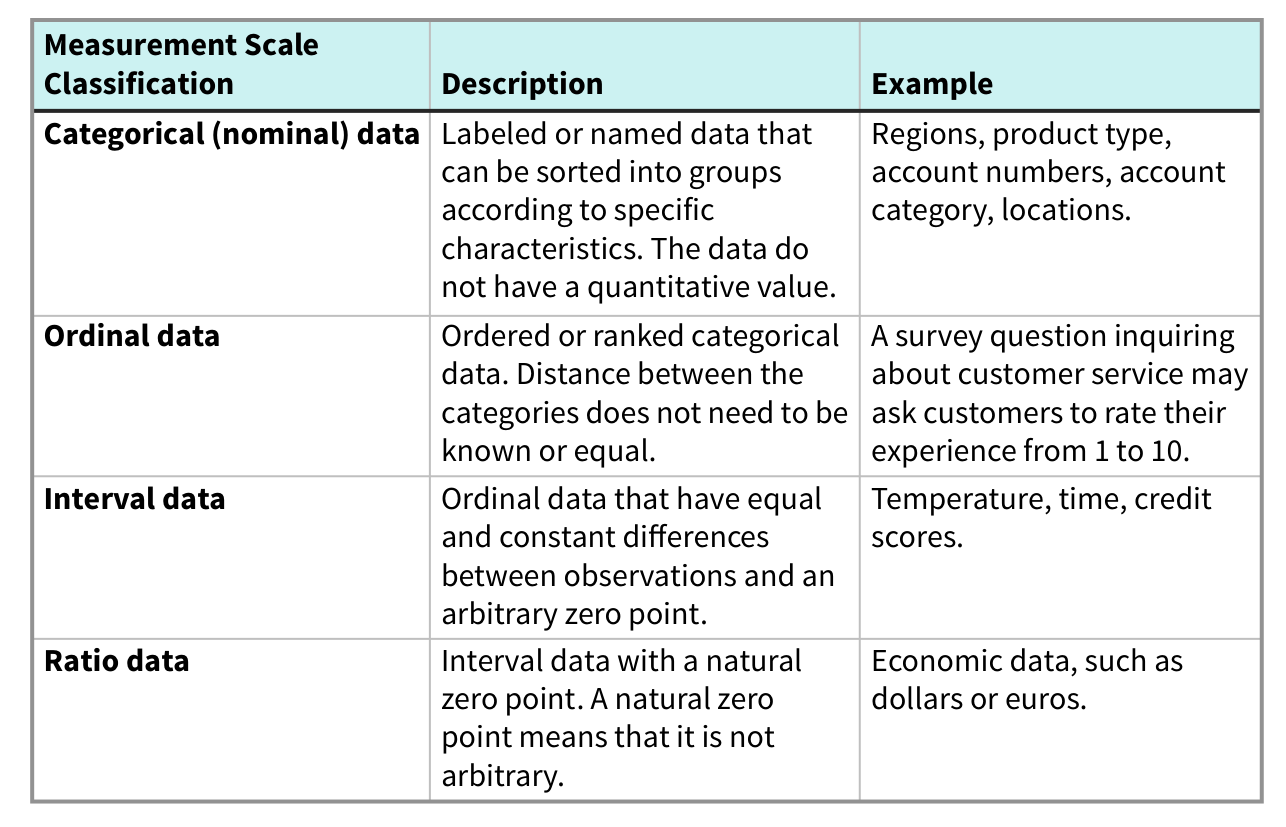
\includegraphics[width=0.95\textwidth,height=0.75\textheight,keepaspectratio]{../textbookForPractice/Figures/Ch_04/ILLUSTRATION 4.11.png}
    \end{figure}
\end{frame}

\begin{frame}{ILLUSTRATION 4.12}
    \begin{figure}[h]
        \centering
        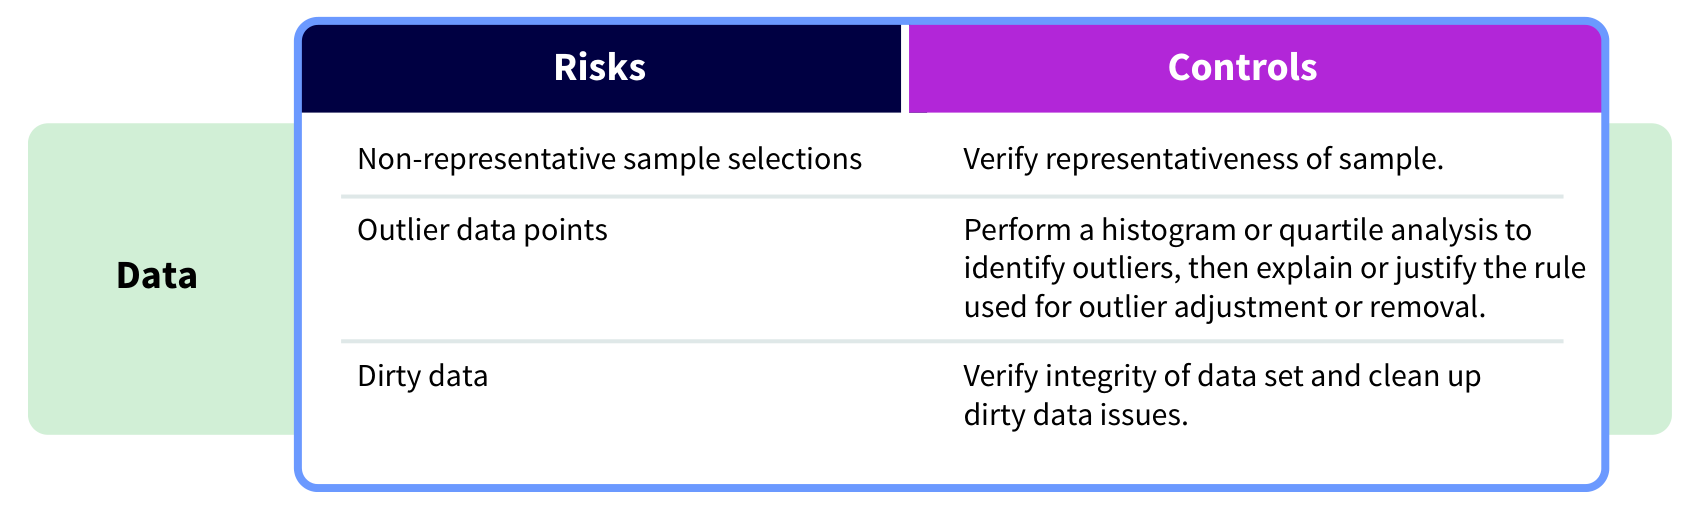
\includegraphics[width=0.95\textwidth,height=0.75\textheight,keepaspectratio]{../textbookForPractice/Figures/Ch_04/ILLUSTRATION 4.12.png}
    \end{figure}
\end{frame}

\begin{frame}{ILLUSTRATION 4.13}
    \begin{figure}[h]
        \centering
        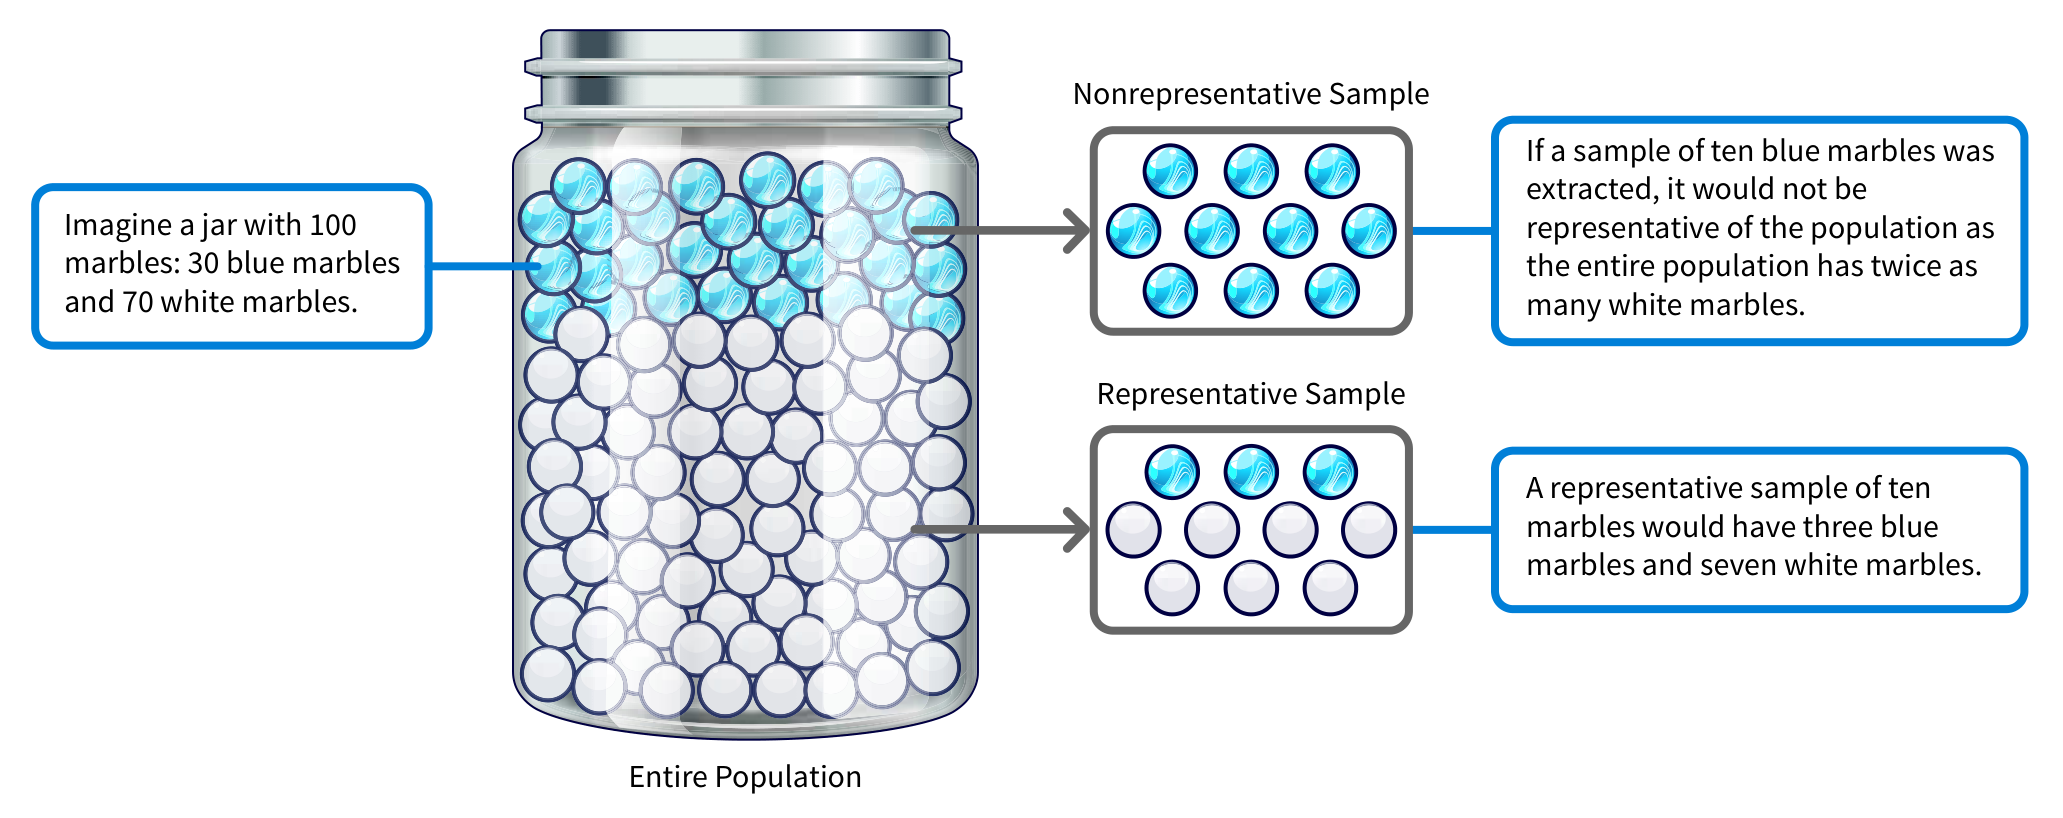
\includegraphics[width=0.95\textwidth,height=0.75\textheight,keepaspectratio]{../textbookForPractice/Figures/Ch_04/ILLUSTRATION 4.13.png}
    \end{figure}
\end{frame}

\begin{frame}{ILLUSTRATION 4.14A}
    \begin{figure}[h]
        \centering
        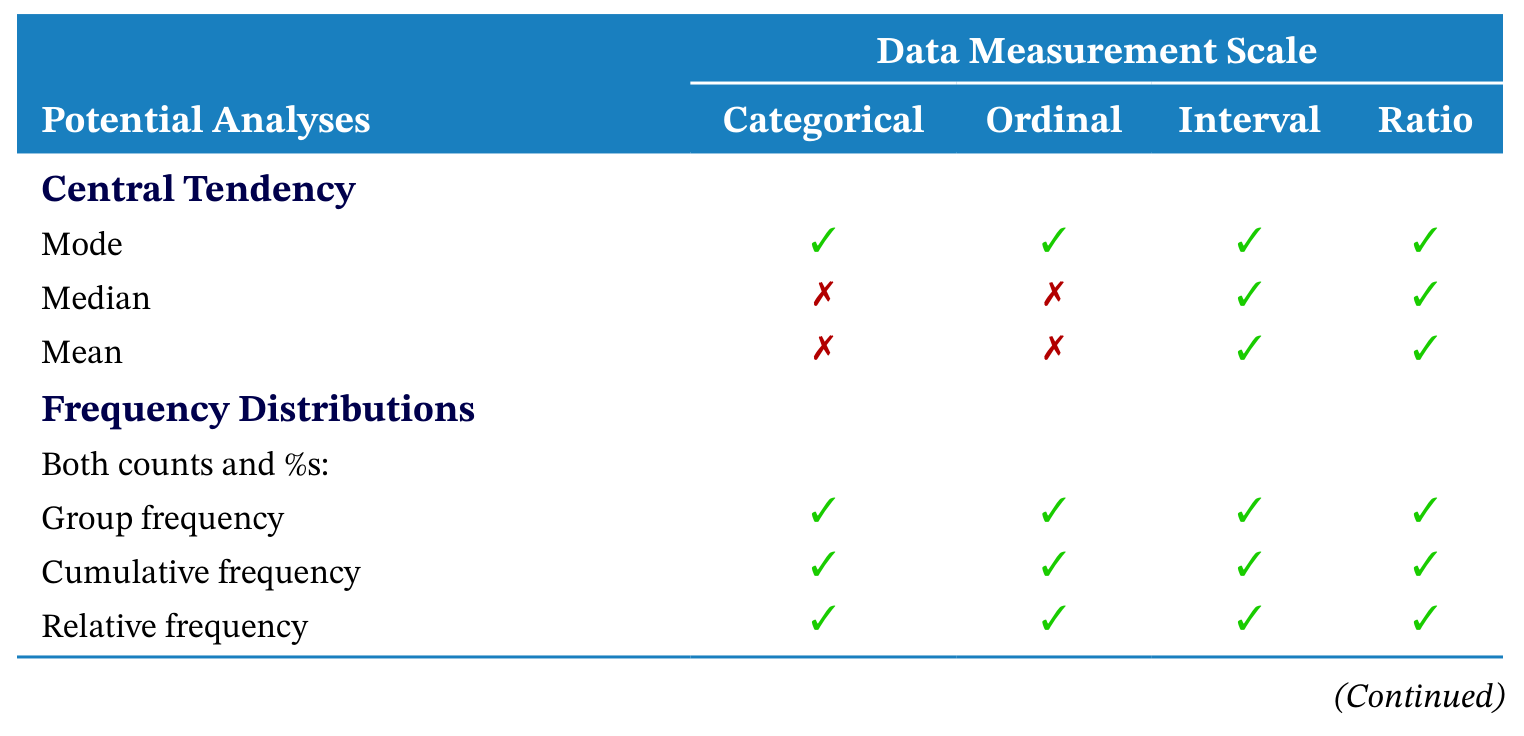
\includegraphics[width=0.95\textwidth,height=0.75\textheight,keepaspectratio]{../textbookForPractice/Figures/Ch_04/ILLUSTRATION 4.14A.png}
    \end{figure}
\end{frame}

\begin{frame}{ILLUSTRATION 4.14B}
    \begin{figure}[h]
        \centering
        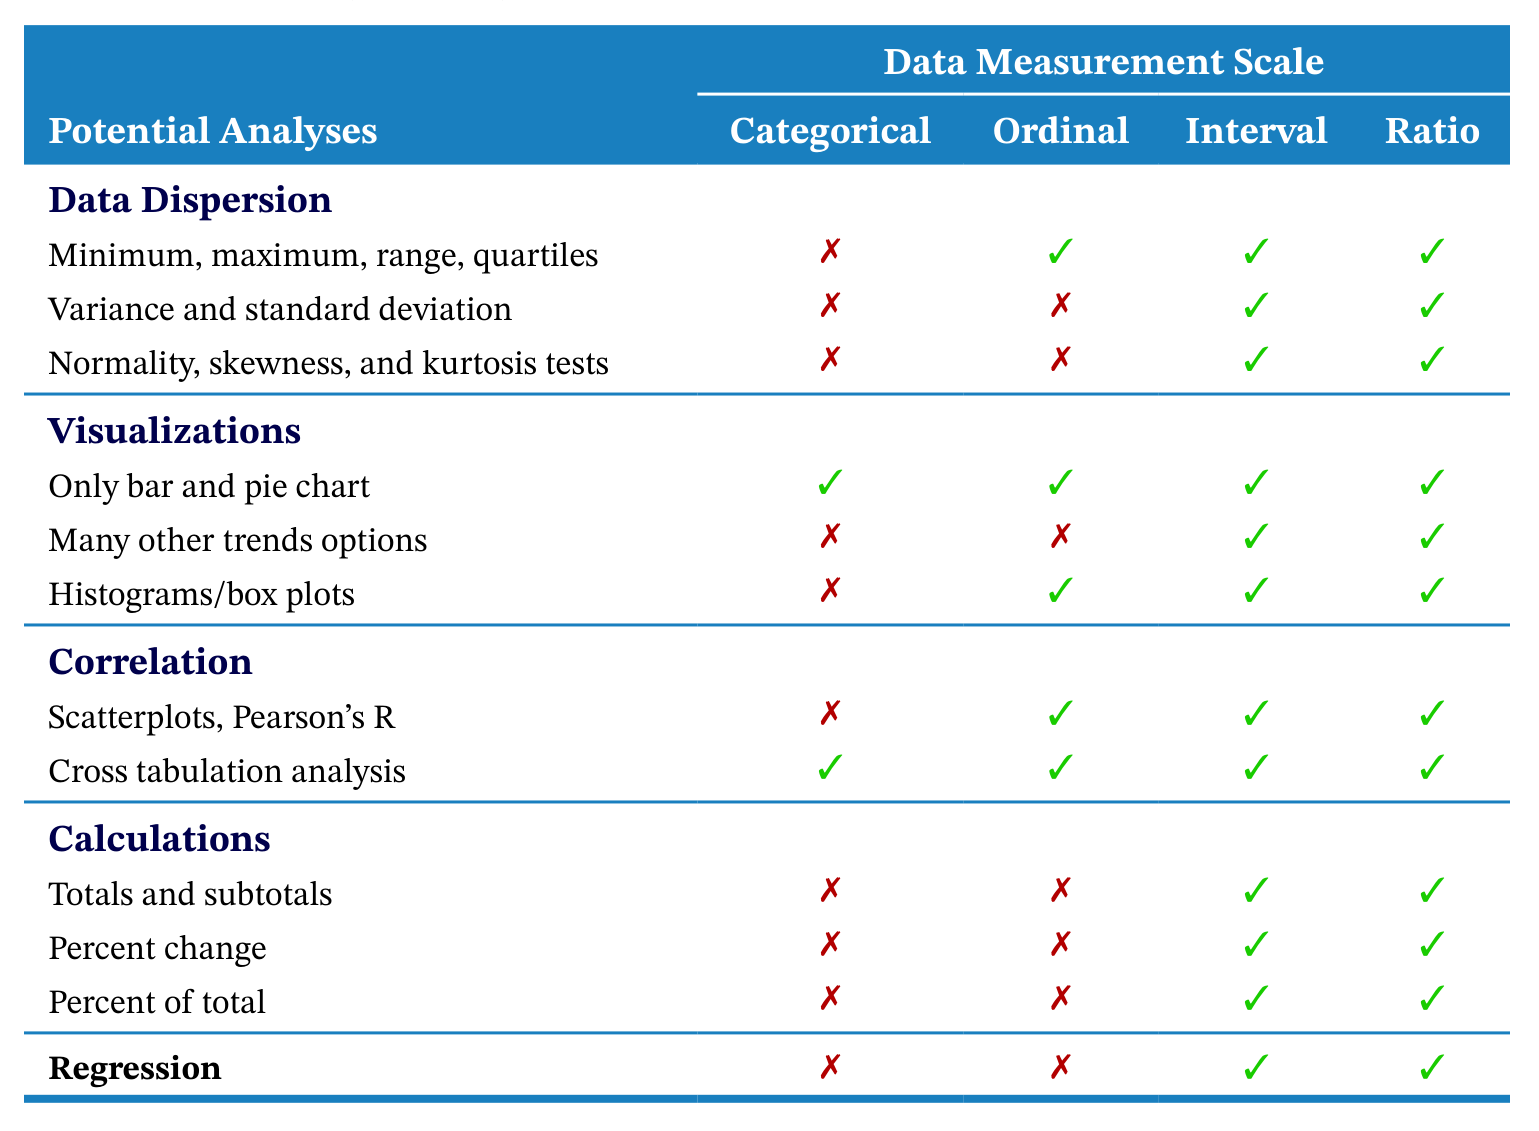
\includegraphics[width=0.95\textwidth,height=0.75\textheight,keepaspectratio]{../textbookForPractice/Figures/Ch_04/ILLUSTRATION 4.14B.png}
    \end{figure}
\end{frame}

\begin{frame}{ILLUSTRATION 4.15}
    \begin{figure}[h]
        \centering
        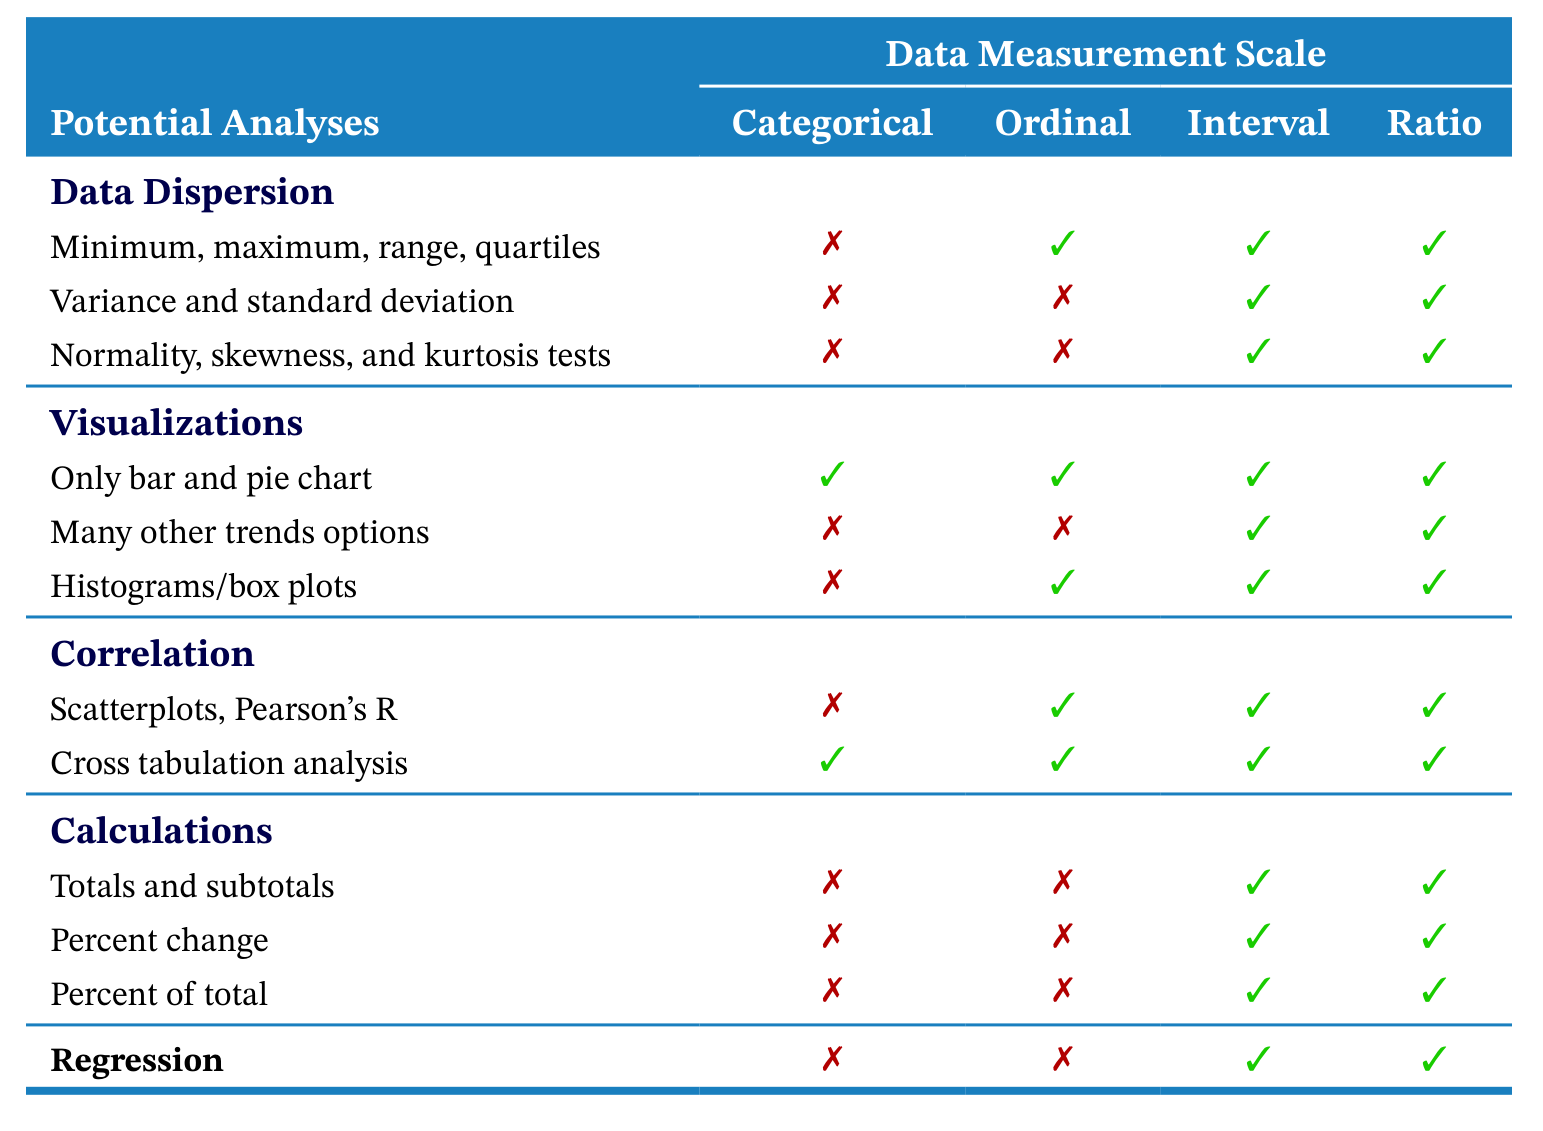
\includegraphics[width=0.95\textwidth,height=0.75\textheight,keepaspectratio]{../textbookForPractice/Figures/Ch_04/ILLUSTRATION 4.15.png}
    \end{figure}
\end{frame}

\begin{frame}{ILLUSTRATION 4.15\_1}
    \begin{figure}[h]
        \centering
        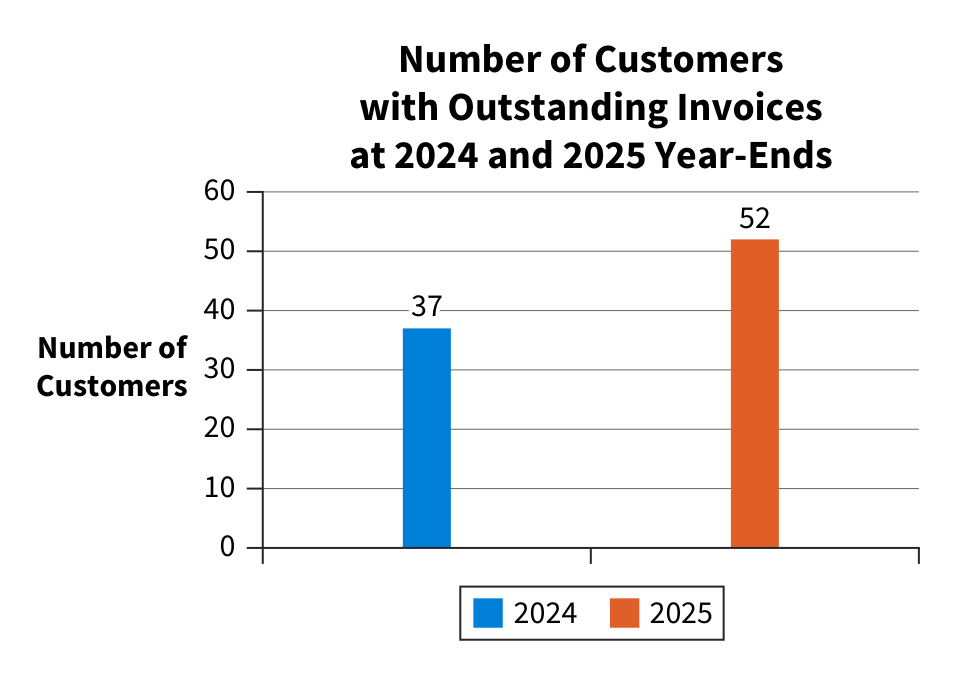
\includegraphics[width=0.95\textwidth,height=0.75\textheight,keepaspectratio]{../textbookForPractice/Figures/Ch_04/ILLUSTRATION 4.15_1.png}
    \end{figure}
\end{frame}

\begin{frame}{ILLUSTRATION 4.15\_2}
    \begin{figure}[h]
        \centering
        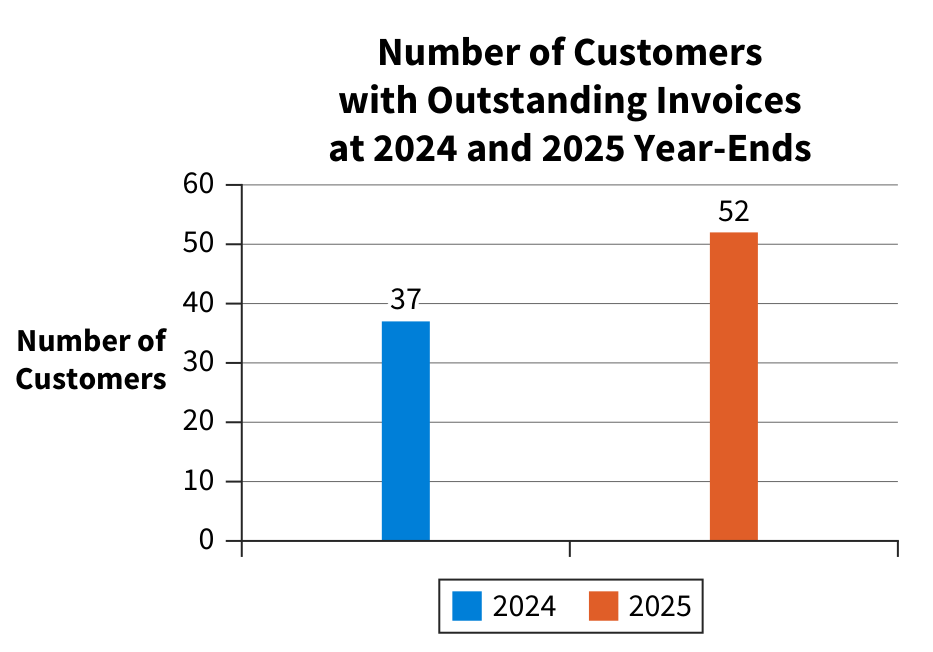
\includegraphics[width=0.95\textwidth,height=0.75\textheight,keepaspectratio]{../textbookForPractice/Figures/Ch_04/ILLUSTRATION 4.15_2.png}
    \end{figure}
\end{frame}

\begin{frame}{ILLUSTRATION 4.16}
    \begin{figure}[h]
        \centering
        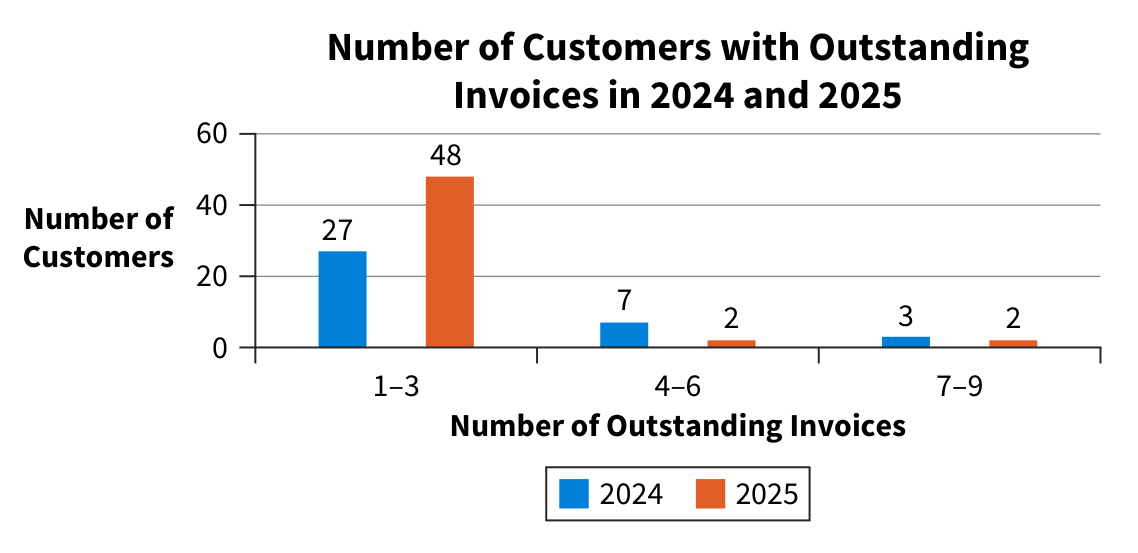
\includegraphics[width=0.95\textwidth,height=0.75\textheight,keepaspectratio]{../textbookForPractice/Figures/Ch_04/ILLUSTRATION 4.16.png}
    \end{figure}
\end{frame}

\begin{frame}{ILLUSTRATION 4.17}
    \begin{figure}[h]
        \centering
        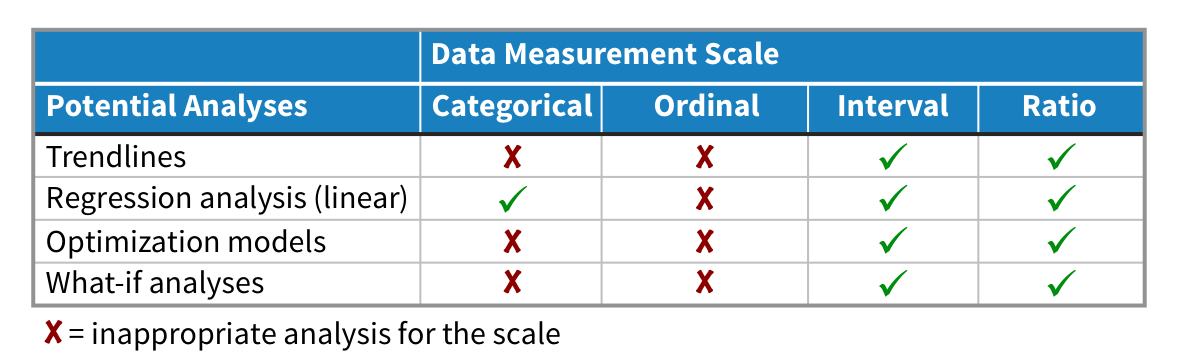
\includegraphics[width=0.95\textwidth,height=0.75\textheight,keepaspectratio]{../textbookForPractice/Figures/Ch_04/ILLUSTRATION 4.17.png}
    \end{figure}
\end{frame}

\begin{frame}{ILLUSTRATION 4.18}
    \begin{figure}[h]
        \centering
        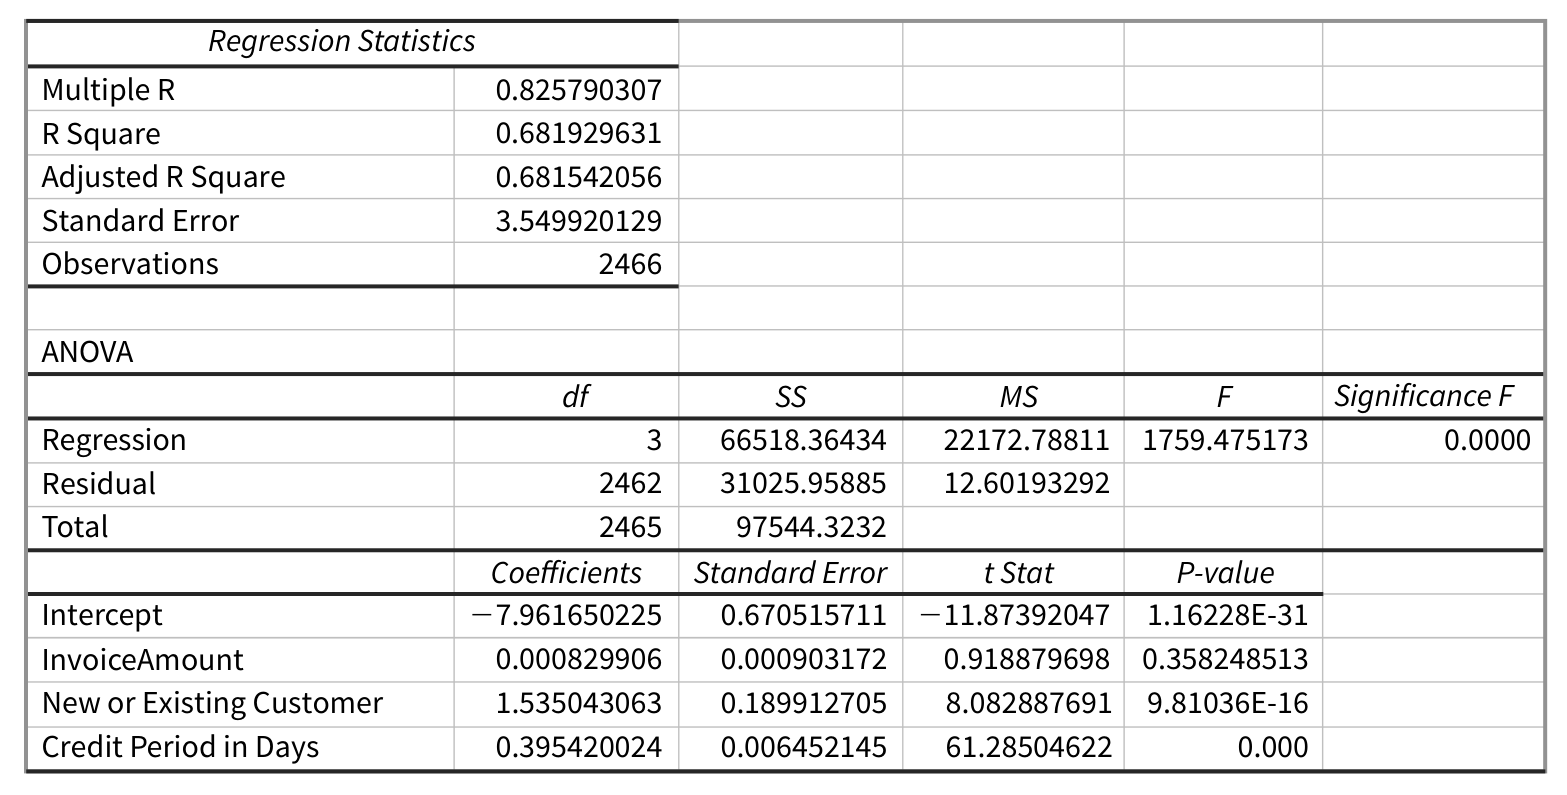
\includegraphics[width=0.95\textwidth,height=0.75\textheight,keepaspectratio]{../textbookForPractice/Figures/Ch_04/ILLUSTRATION 4.18.png}
    \end{figure}
\end{frame}

\begin{frame}{ILLUSTRATION 4.19}
    \begin{figure}[h]
        \centering
        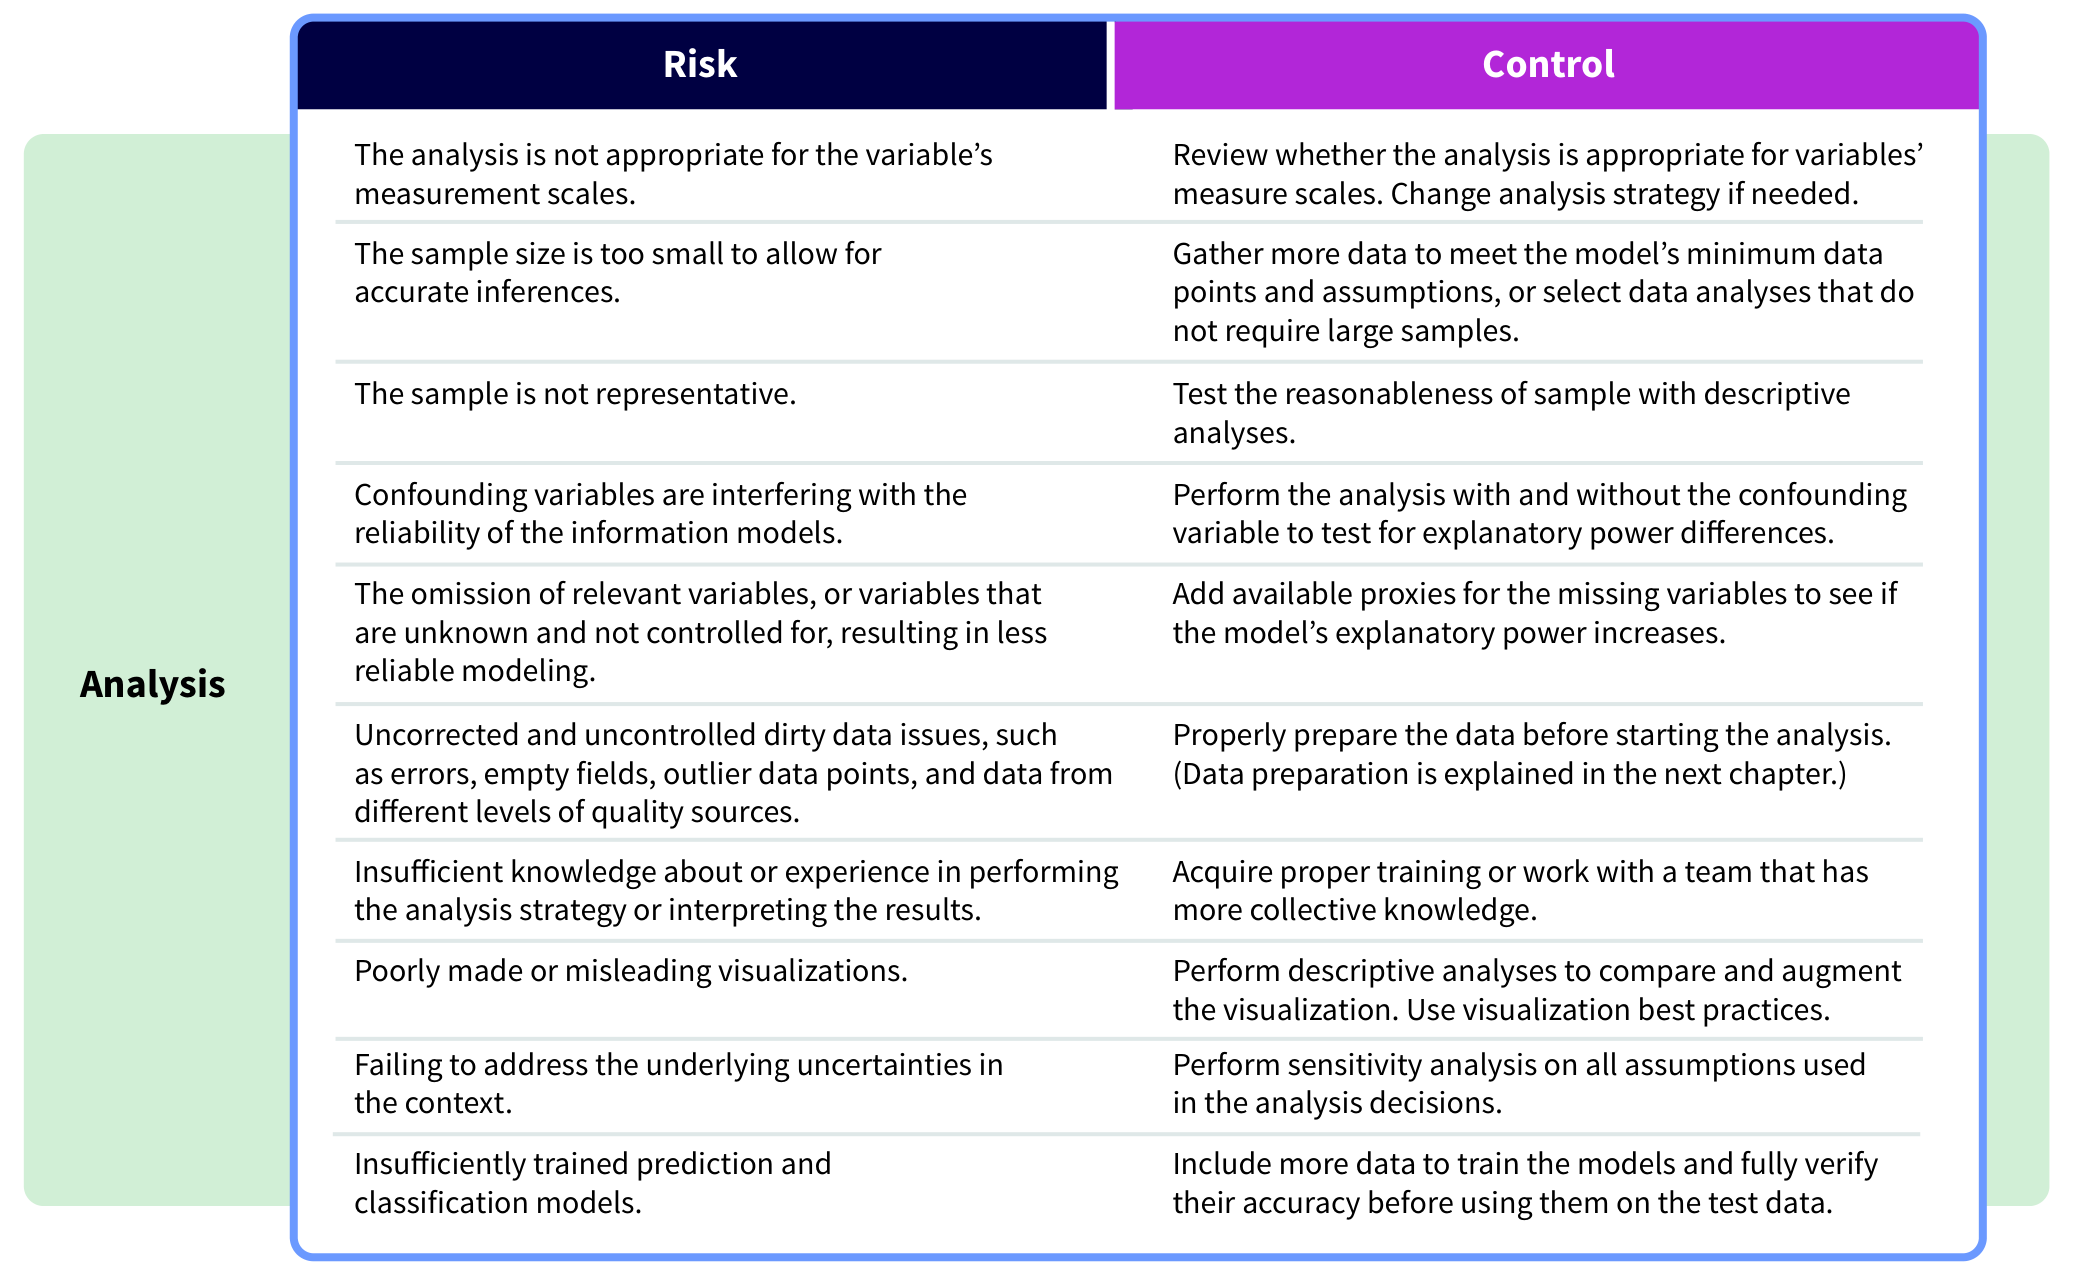
\includegraphics[width=0.95\textwidth,height=0.75\textheight,keepaspectratio]{../textbookForPractice/Figures/Ch_04/ILLUSTRATION 4.19.png}
    \end{figure}
\end{frame}

\begin{frame}{ILLUSTRATION 4.2}
    \begin{figure}[h]
        \centering
        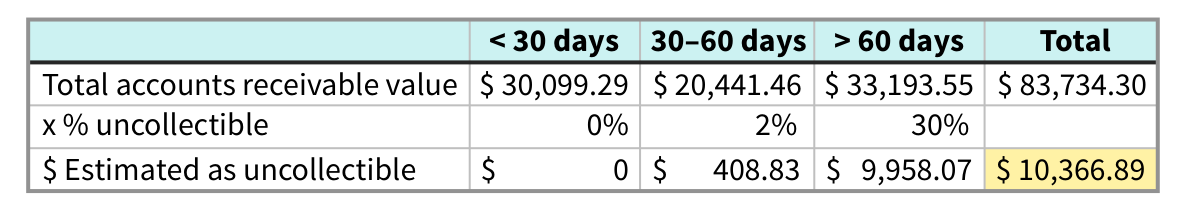
\includegraphics[width=0.95\textwidth,height=0.75\textheight,keepaspectratio]{../textbookForPractice/Figures/Ch_04/ILLUSTRATION 4.2.png}
    \end{figure}
\end{frame}

\begin{frame}{ILLUSTRATION 4.20}
    \begin{figure}[h]
        \centering
        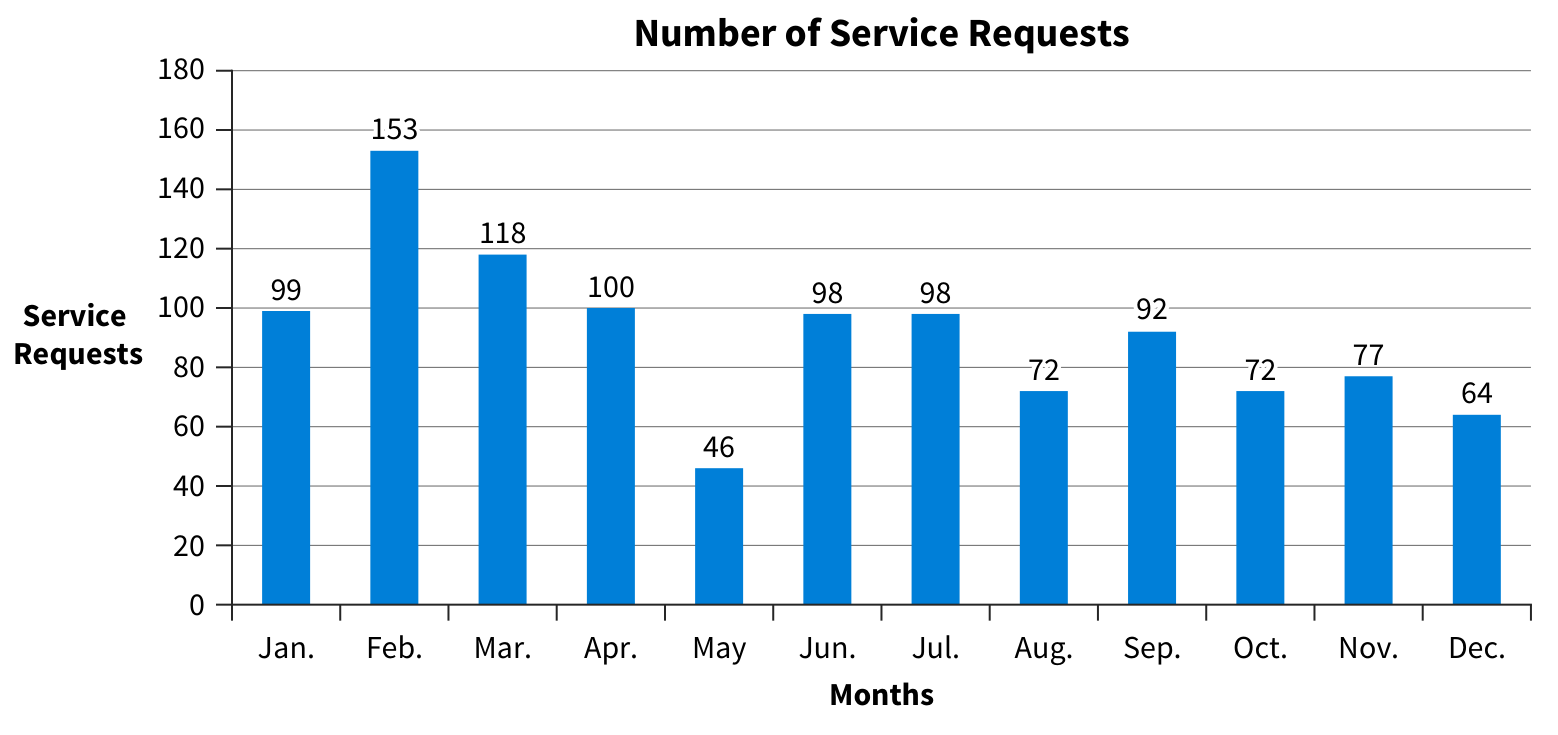
\includegraphics[width=0.95\textwidth,height=0.75\textheight,keepaspectratio]{../textbookForPractice/Figures/Ch_04/ILLUSTRATION 4.20.png}
    \end{figure}
\end{frame}

\begin{frame}{ILLUSTRATION 4.21}
    \begin{figure}[h]
        \centering
        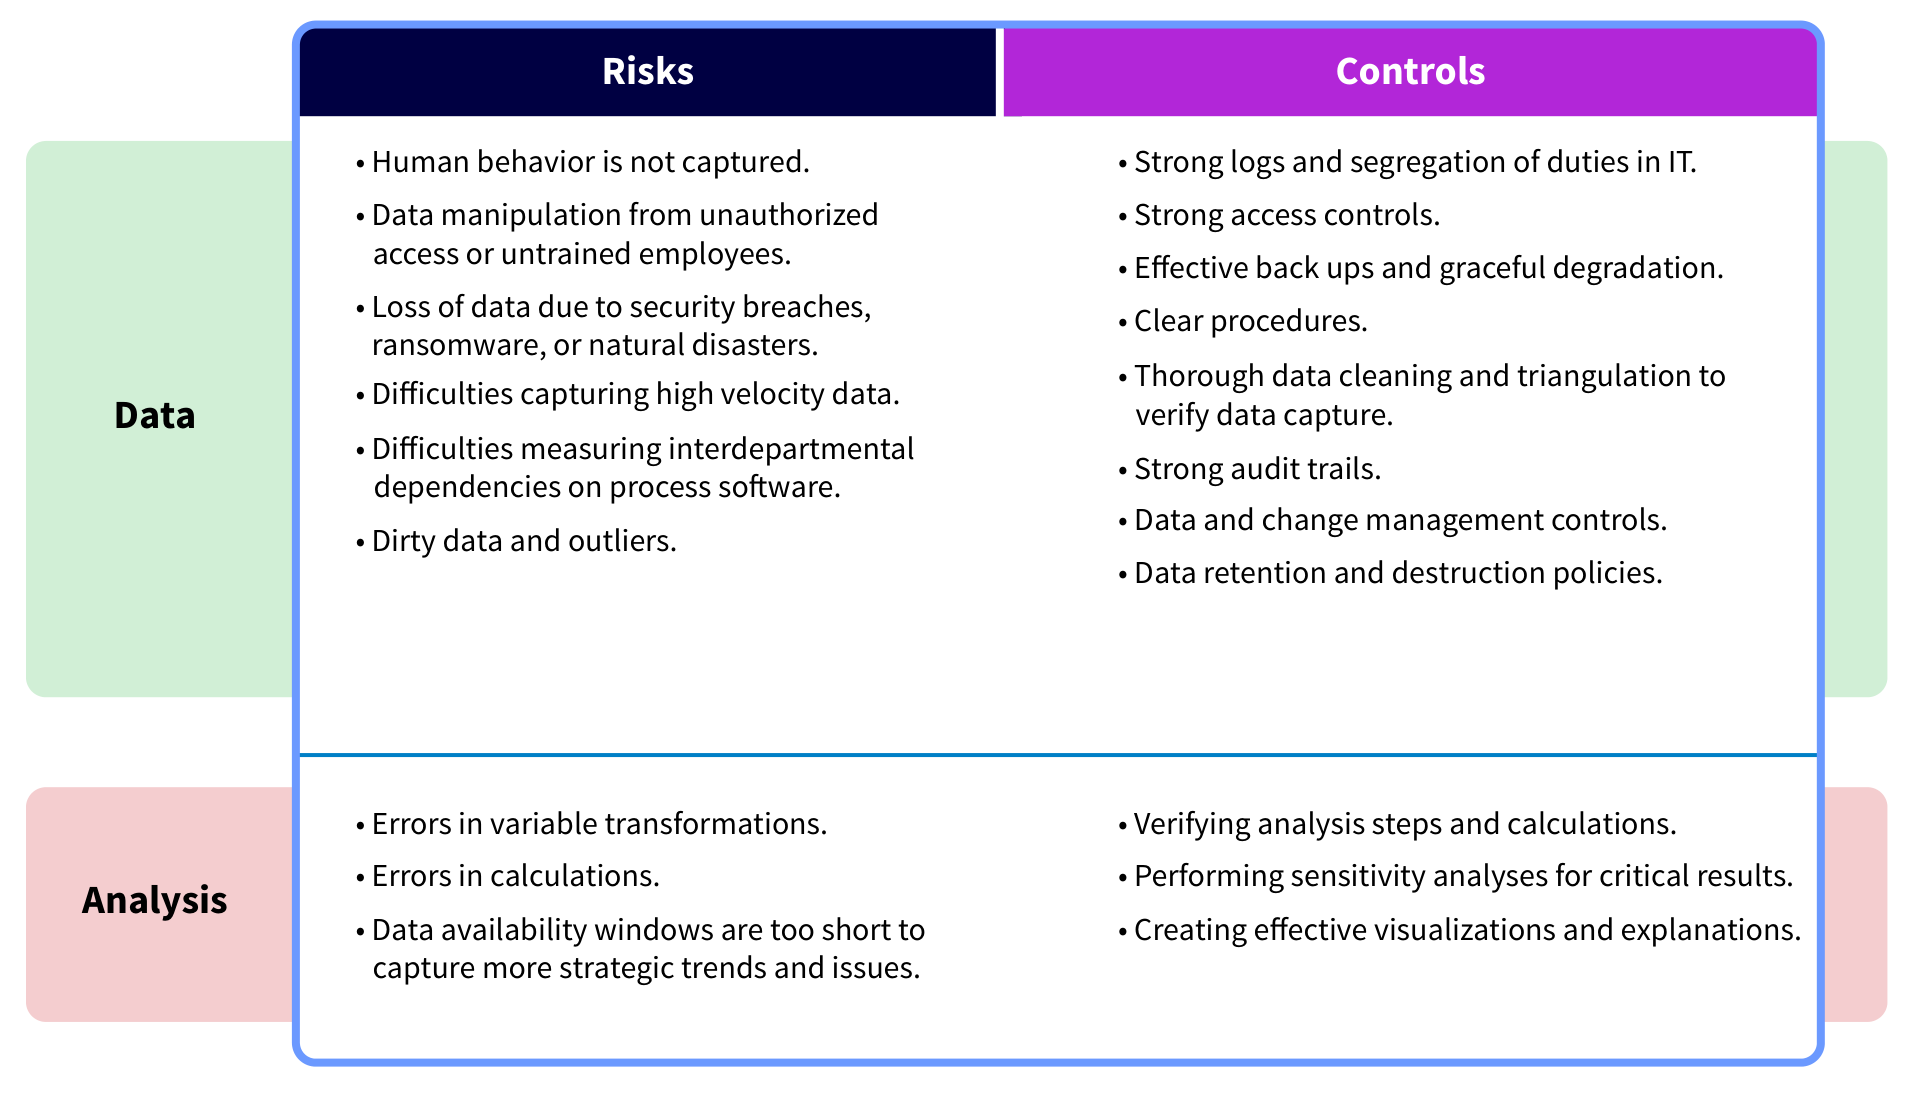
\includegraphics[width=0.95\textwidth,height=0.75\textheight,keepaspectratio]{../textbookForPractice/Figures/Ch_04/ILLUSTRATION 4.21.png}
    \end{figure}
\end{frame}

\begin{frame}{ILLUSTRATION 4.22}
    \begin{figure}[h]
        \centering
        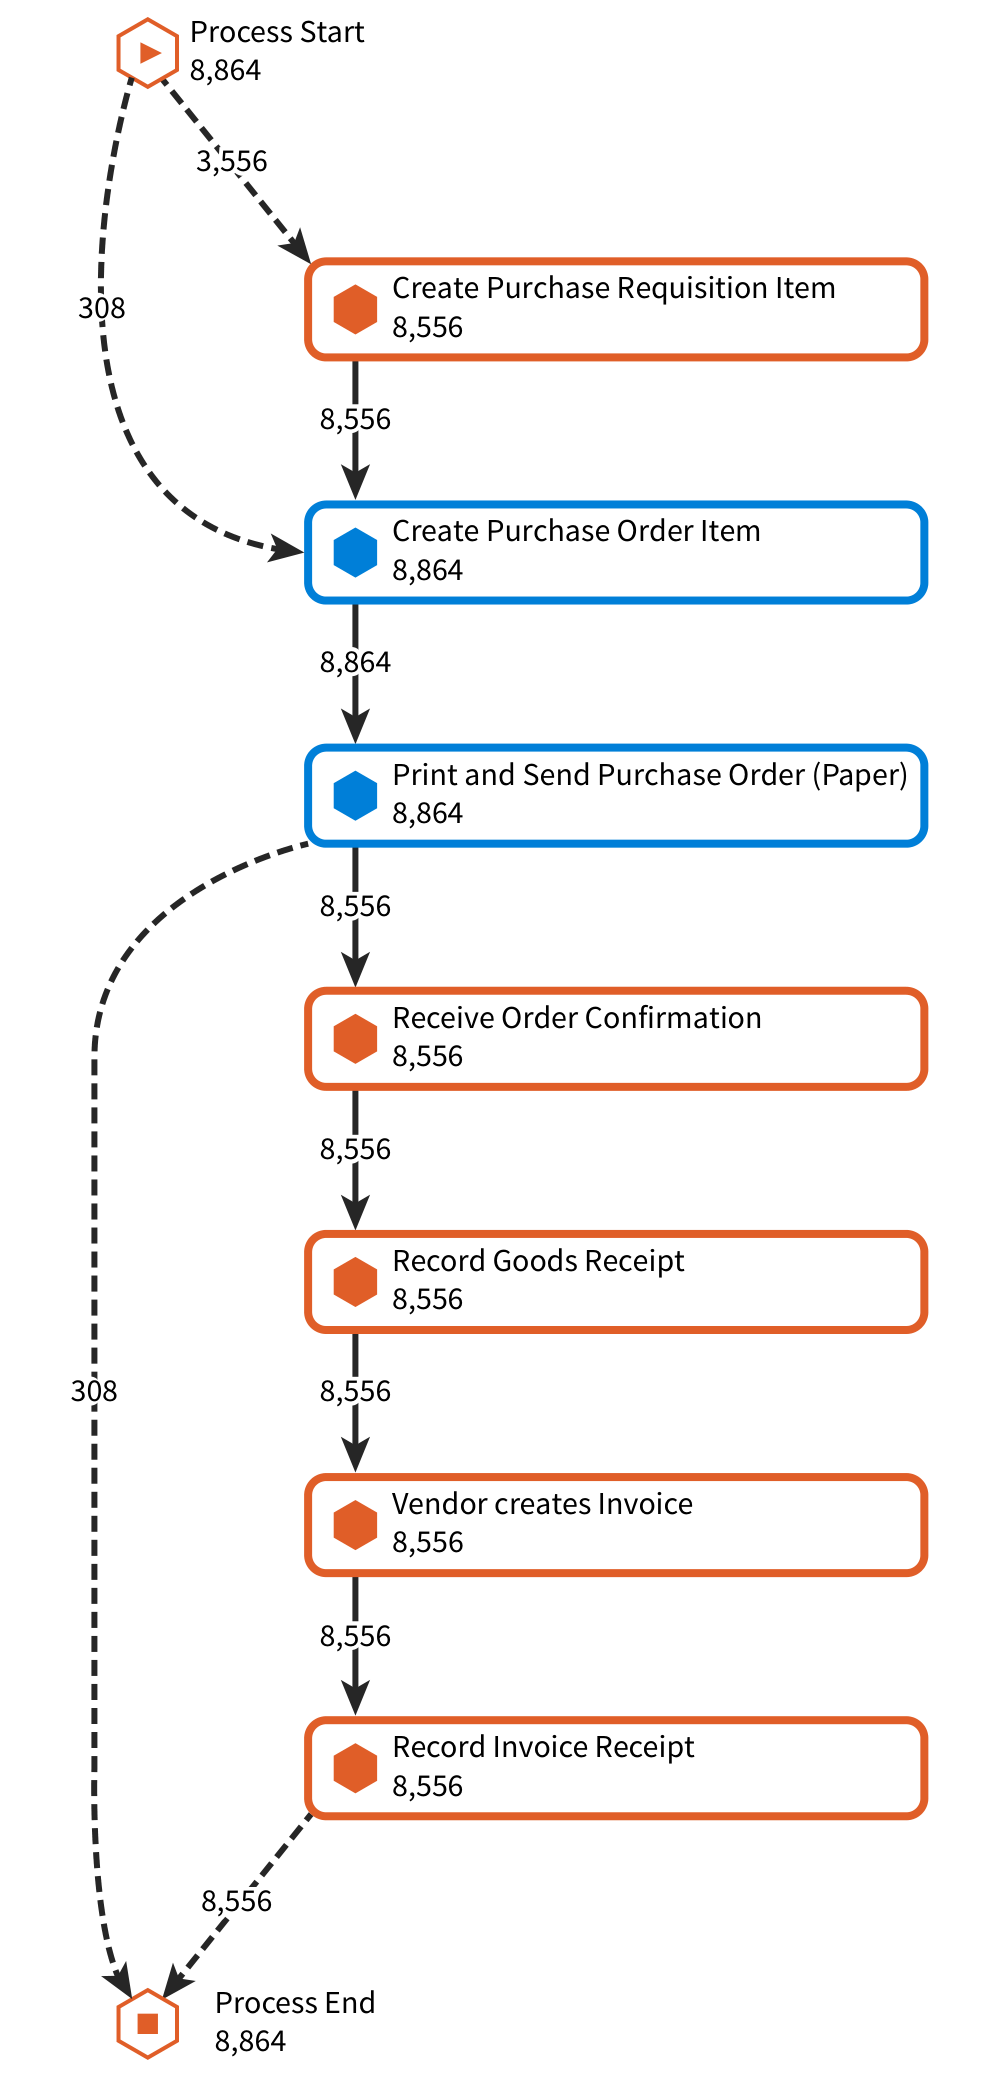
\includegraphics[width=0.95\textwidth,height=0.75\textheight,keepaspectratio]{../textbookForPractice/Figures/Ch_04/ILLUSTRATION 4.22.png}
    \end{figure}
\end{frame}

\begin{frame}{ILLUSTRATION 4.23}
    \begin{figure}[h]
        \centering
        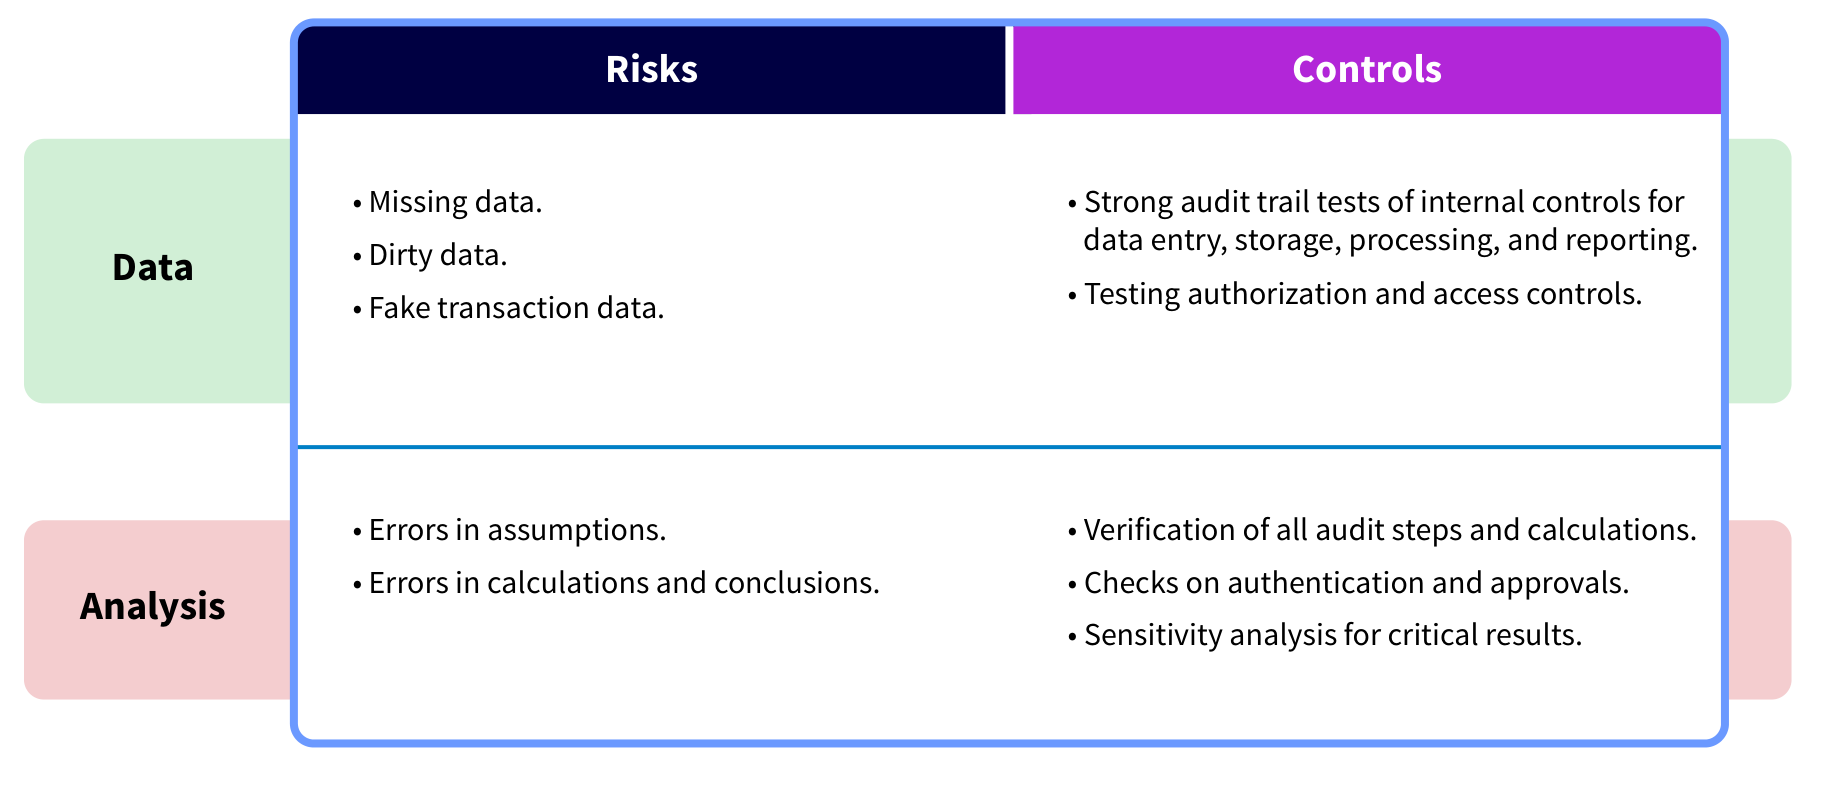
\includegraphics[width=0.95\textwidth,height=0.75\textheight,keepaspectratio]{../textbookForPractice/Figures/Ch_04/ILLUSTRATION 4.23.png}
    \end{figure}
\end{frame}

\begin{frame}{ILLUSTRATION 4.24}
    \begin{figure}[h]
        \centering
        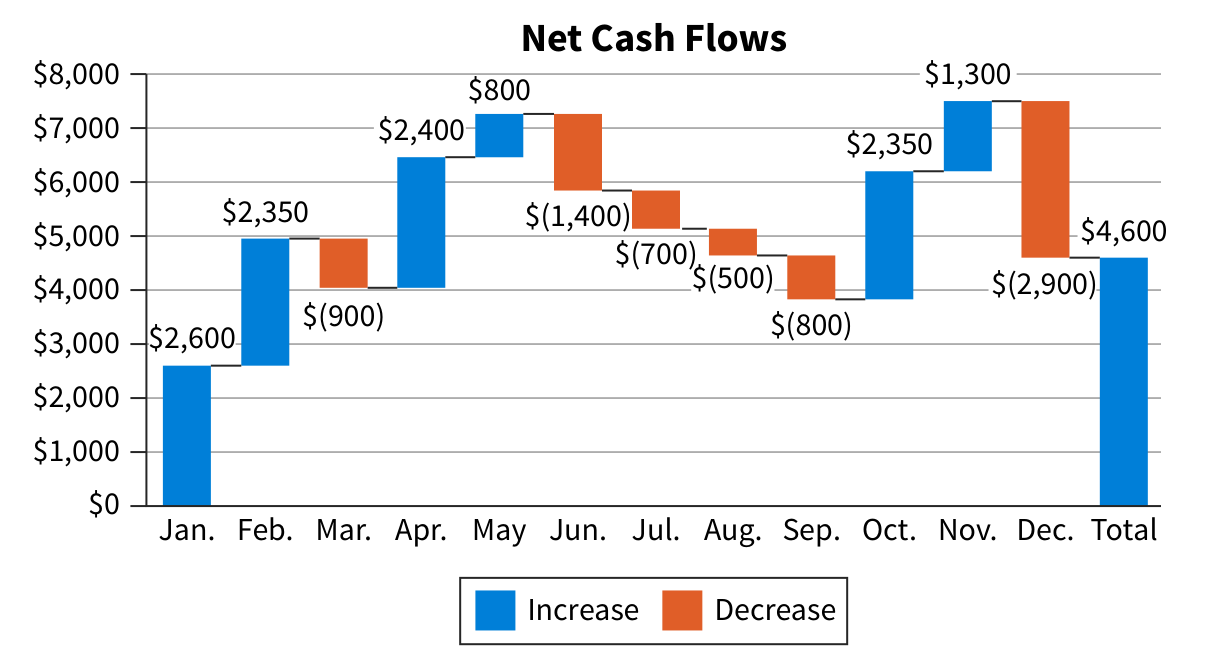
\includegraphics[width=0.95\textwidth,height=0.75\textheight,keepaspectratio]{../textbookForPractice/Figures/Ch_04/ILLUSTRATION 4.24.png}
    \end{figure}
\end{frame}

\begin{frame}{ILLUSTRATION 4.25}
    \begin{figure}[h]
        \centering
        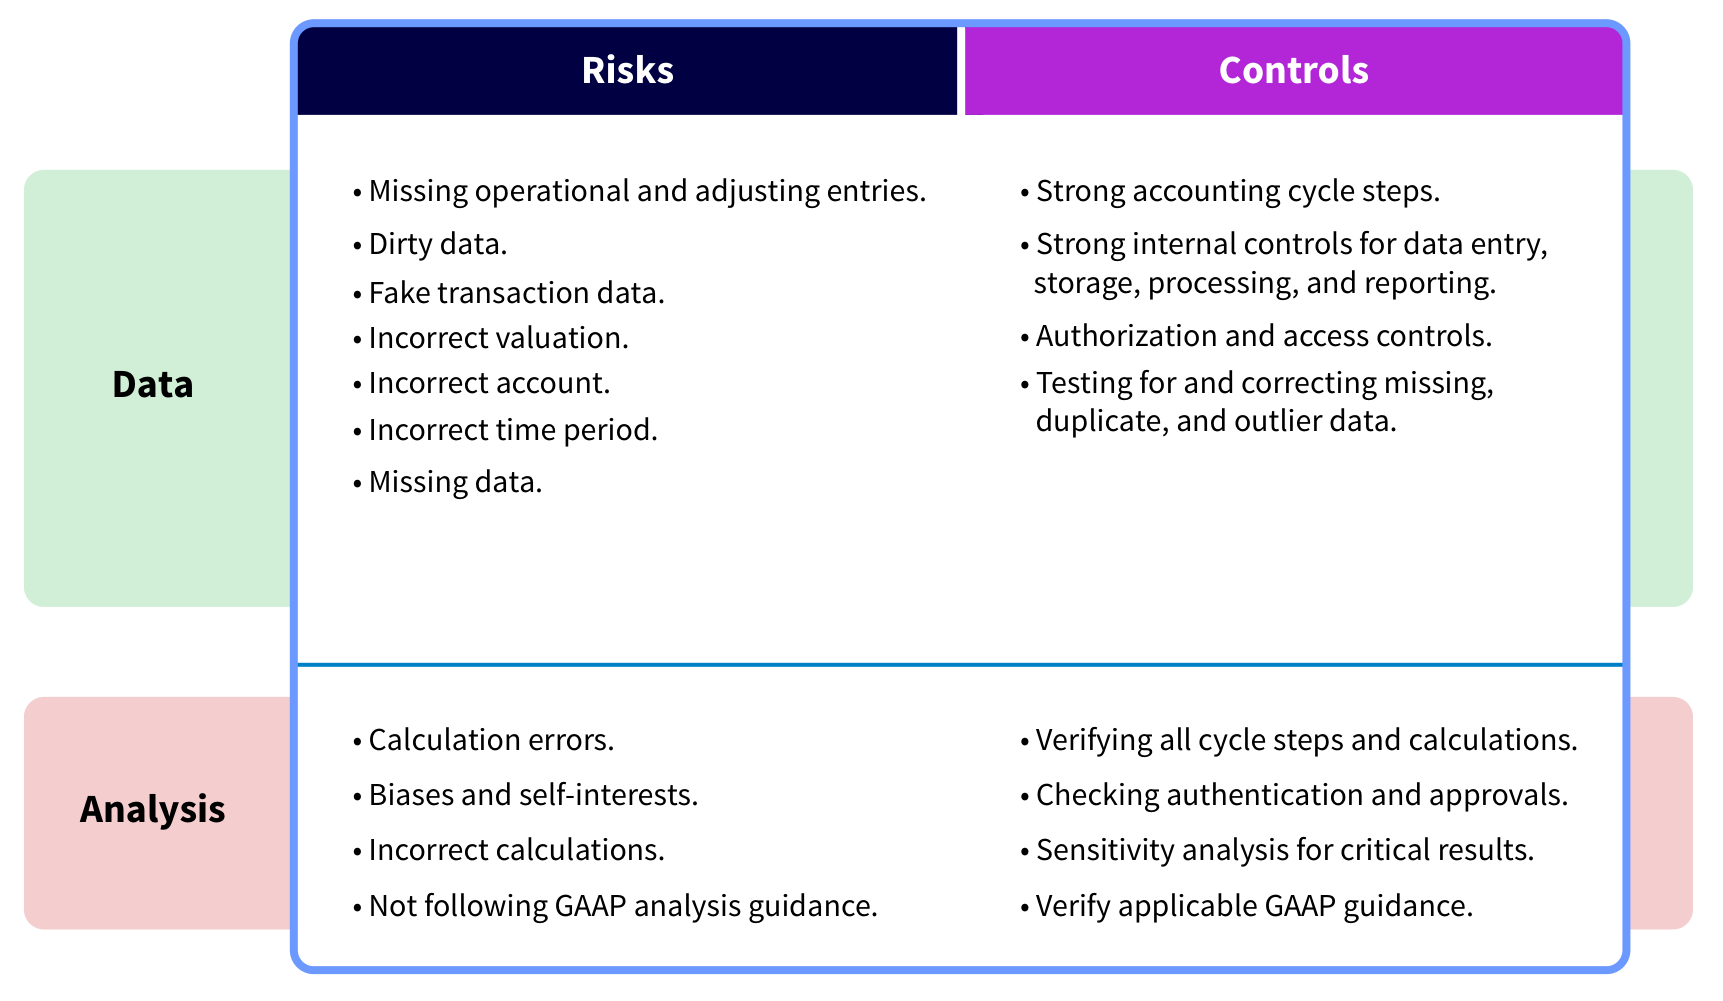
\includegraphics[width=0.95\textwidth,height=0.75\textheight,keepaspectratio]{../textbookForPractice/Figures/Ch_04/ILLUSTRATION 4.25.png}
    \end{figure}
\end{frame}

\begin{frame}{ILLUSTRATION 4.26}
    \begin{figure}[h]
        \centering
        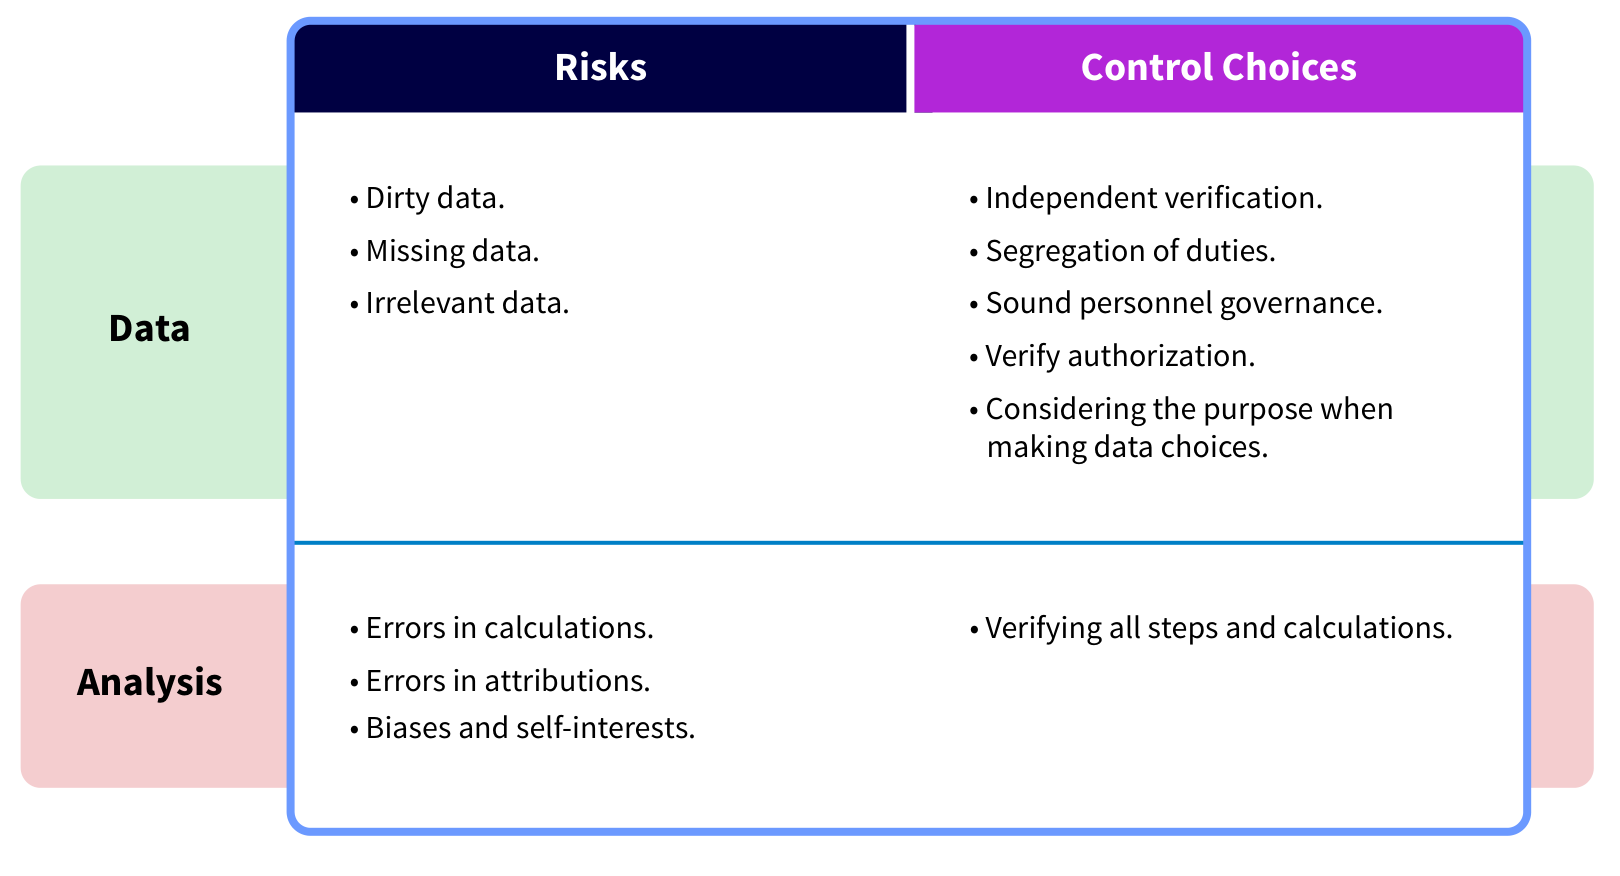
\includegraphics[width=0.95\textwidth,height=0.75\textheight,keepaspectratio]{../textbookForPractice/Figures/Ch_04/ILLUSTRATION 4.26.png}
    \end{figure}
\end{frame}

\begin{frame}{ILLUSTRATION 4.27}
    \begin{figure}[h]
        \centering
        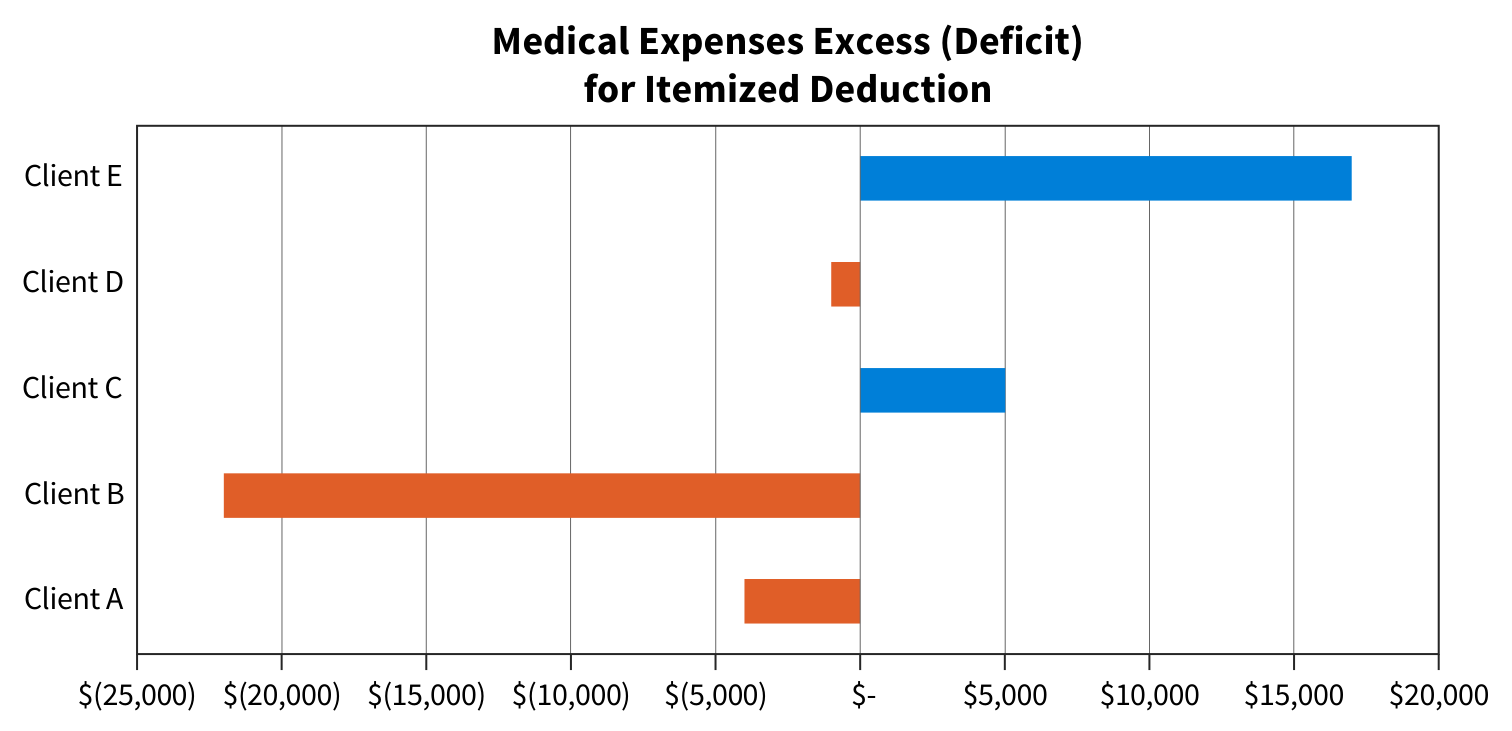
\includegraphics[width=0.95\textwidth,height=0.75\textheight,keepaspectratio]{../textbookForPractice/Figures/Ch_04/ILLUSTRATION 4.27.png}
    \end{figure}
\end{frame}

\begin{frame}{ILLUSTRATION 4.28}
    \begin{figure}[h]
        \centering
        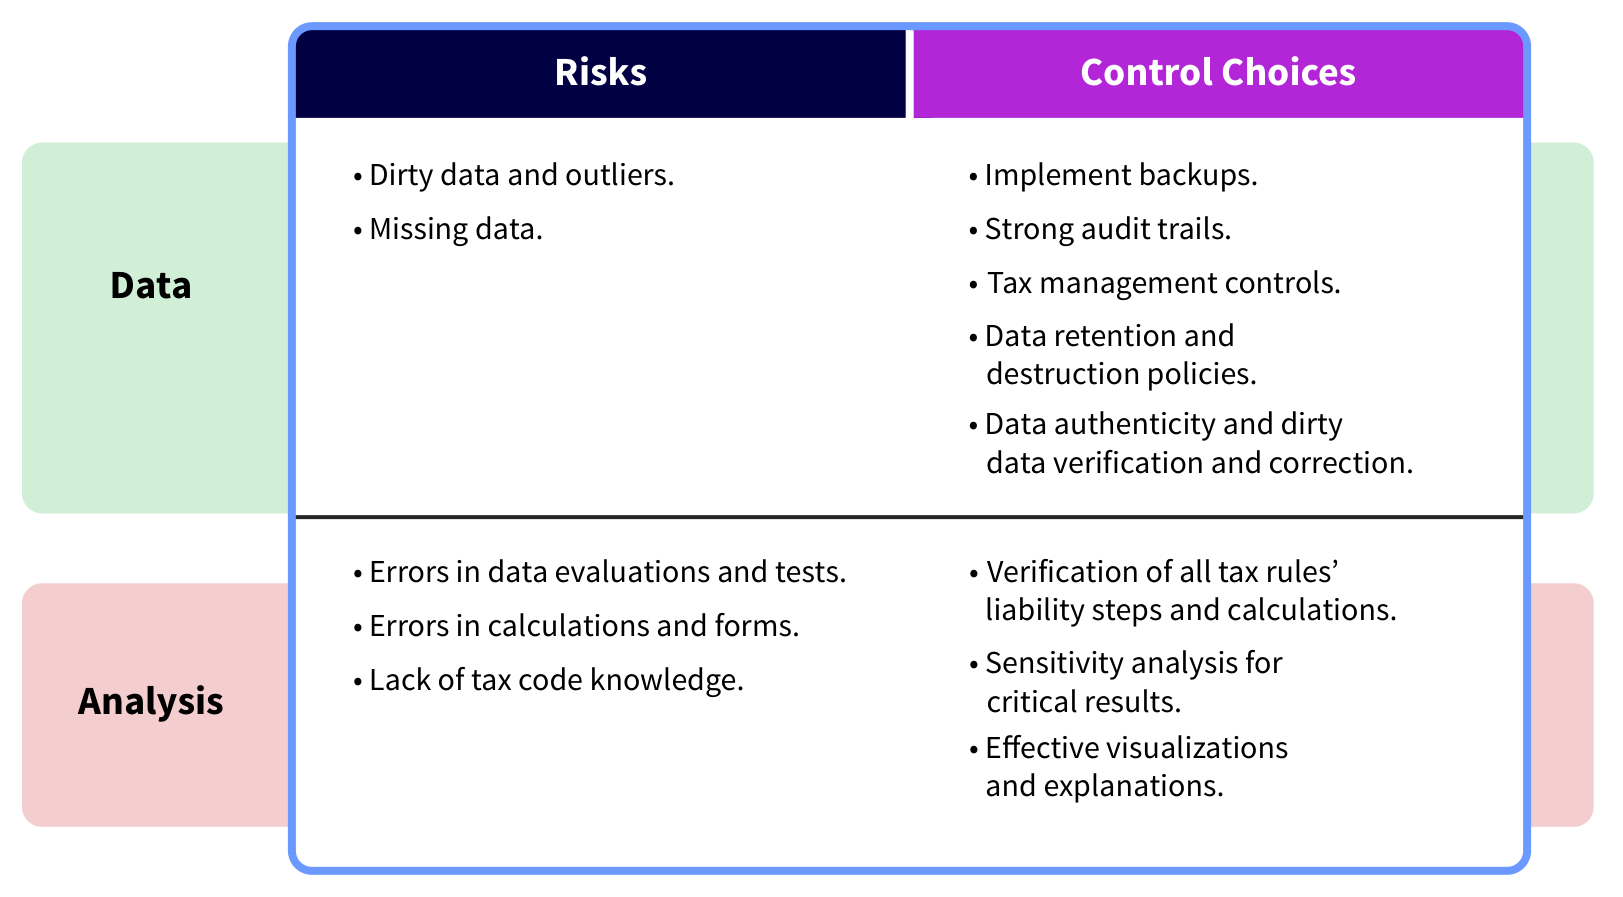
\includegraphics[width=0.95\textwidth,height=0.75\textheight,keepaspectratio]{../textbookForPractice/Figures/Ch_04/ILLUSTRATION 4.28.png}
    \end{figure}
\end{frame}

\begin{frame}{ILLUSTRATION 4.29}
    \begin{figure}[h]
        \centering
        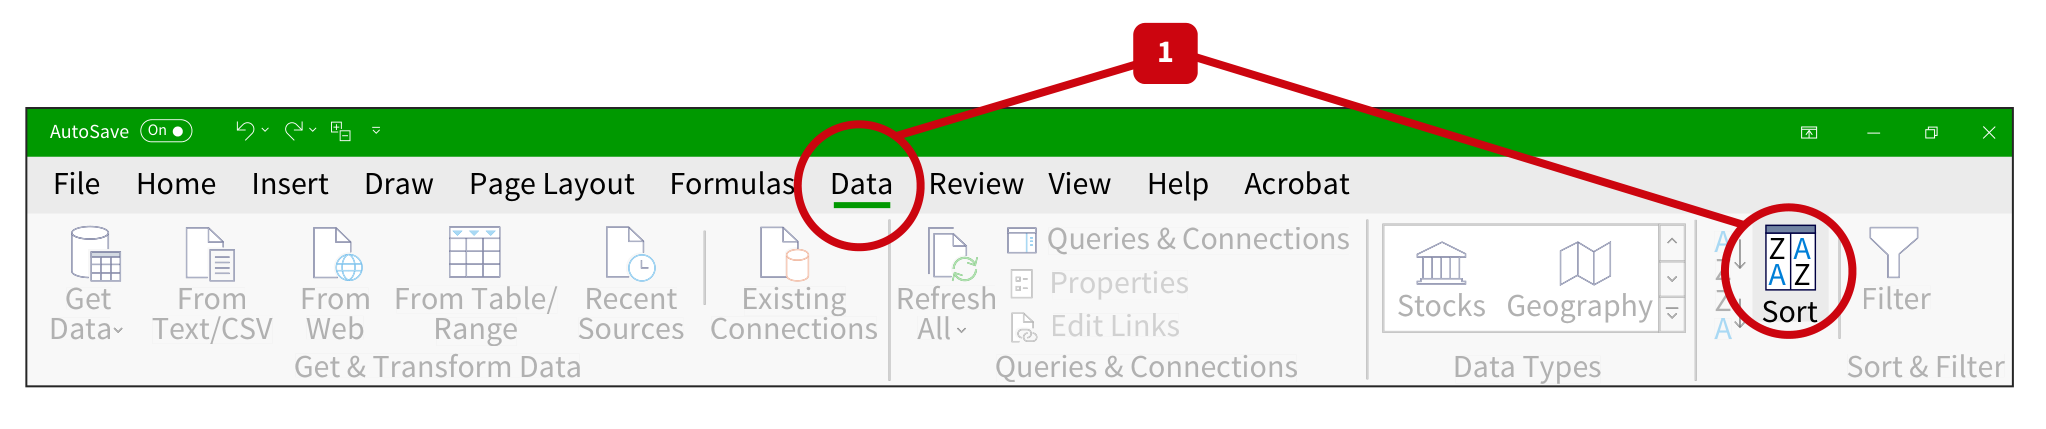
\includegraphics[width=0.95\textwidth,height=0.75\textheight,keepaspectratio]{../textbookForPractice/Figures/Ch_04/ILLUSTRATION 4.29.png}
    \end{figure}
\end{frame}

\begin{frame}{ILLUSTRATION 4.3}
    \begin{figure}[h]
        \centering
        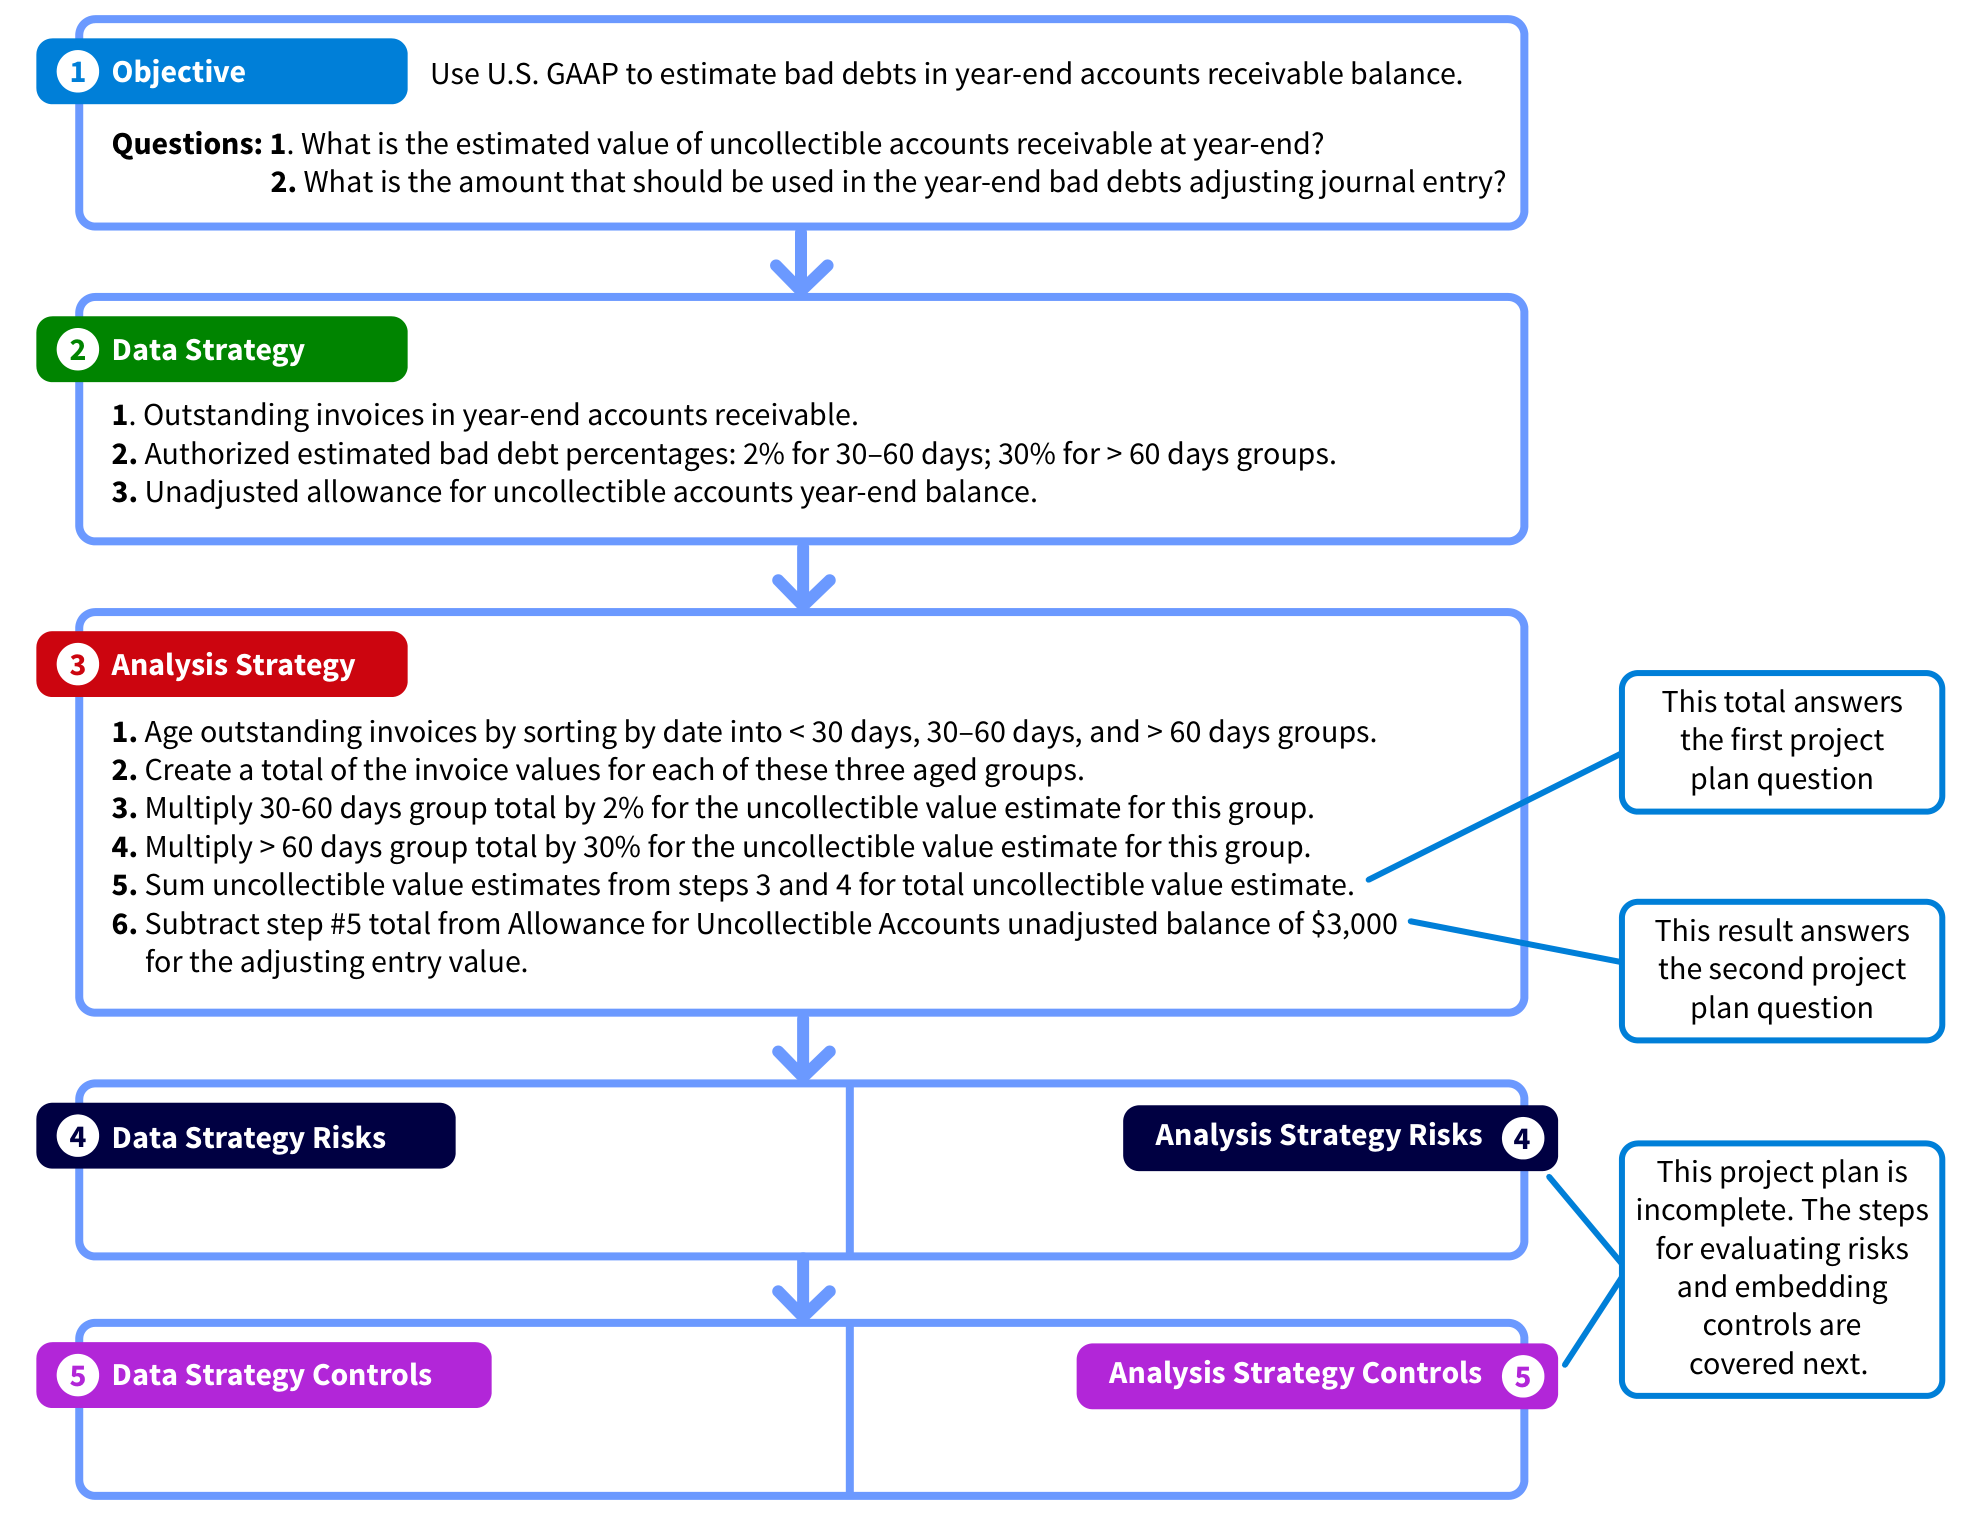
\includegraphics[width=0.95\textwidth,height=0.75\textheight,keepaspectratio]{../textbookForPractice/Figures/Ch_04/ILLUSTRATION 4.3.png}
    \end{figure}
\end{frame}

\begin{frame}{ILLUSTRATION 4.30}
    \begin{figure}[h]
        \centering
        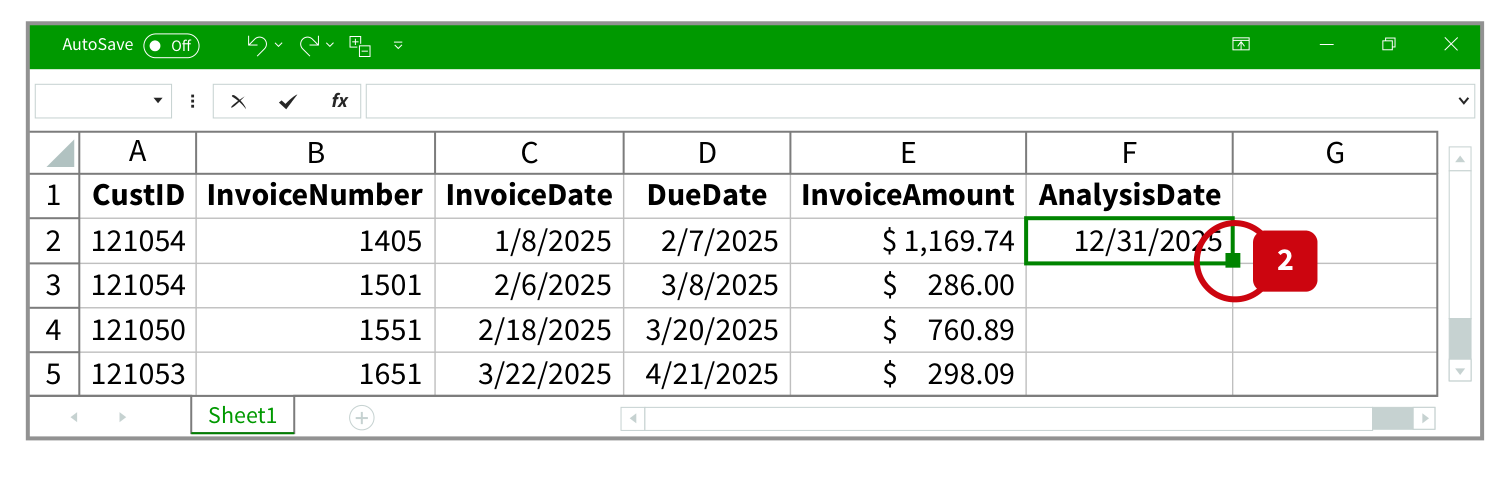
\includegraphics[width=0.95\textwidth,height=0.75\textheight,keepaspectratio]{../textbookForPractice/Figures/Ch_04/ILLUSTRATION 4.30.png}
    \end{figure}
\end{frame}

\begin{frame}{ILLUSTRATION 4.31}
    \begin{figure}[h]
        \centering
        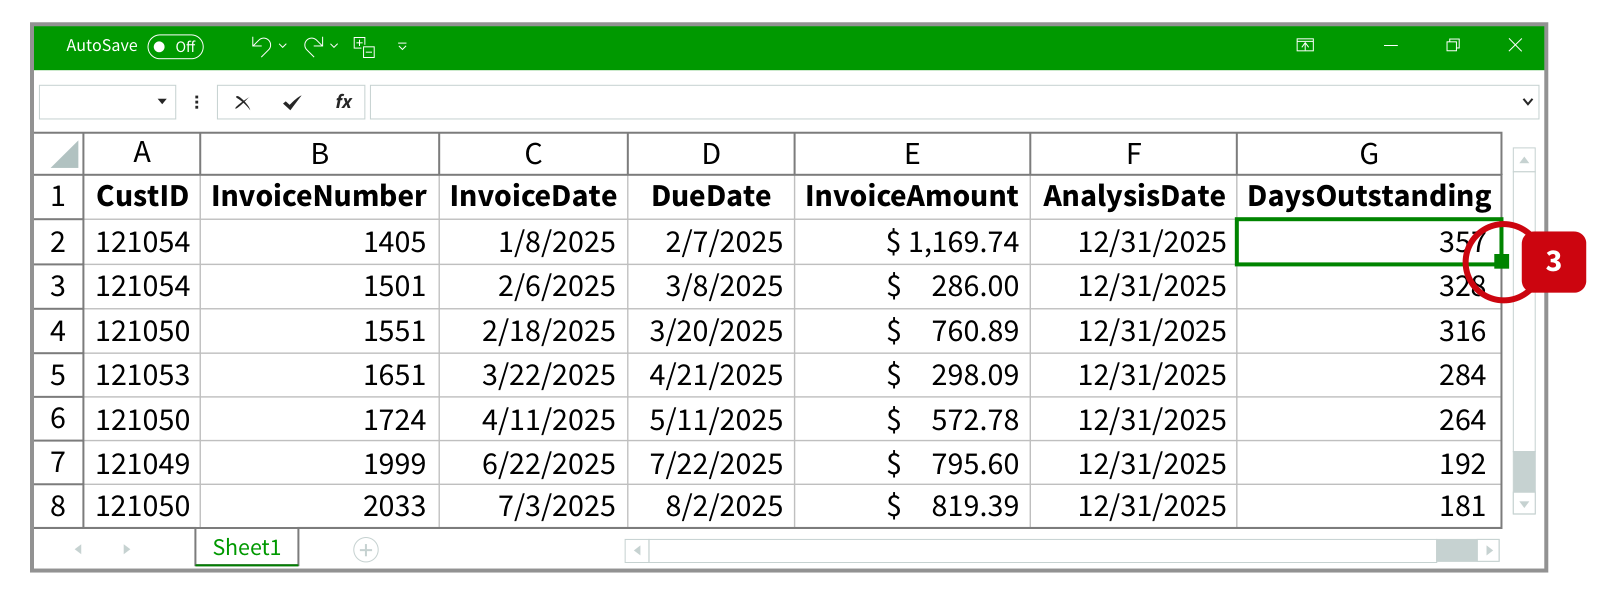
\includegraphics[width=0.95\textwidth,height=0.75\textheight,keepaspectratio]{../textbookForPractice/Figures/Ch_04/ILLUSTRATION 4.31.png}
    \end{figure}
\end{frame}

\begin{frame}{ILLUSTRATION 4.32}
    \begin{figure}[h]
        \centering
        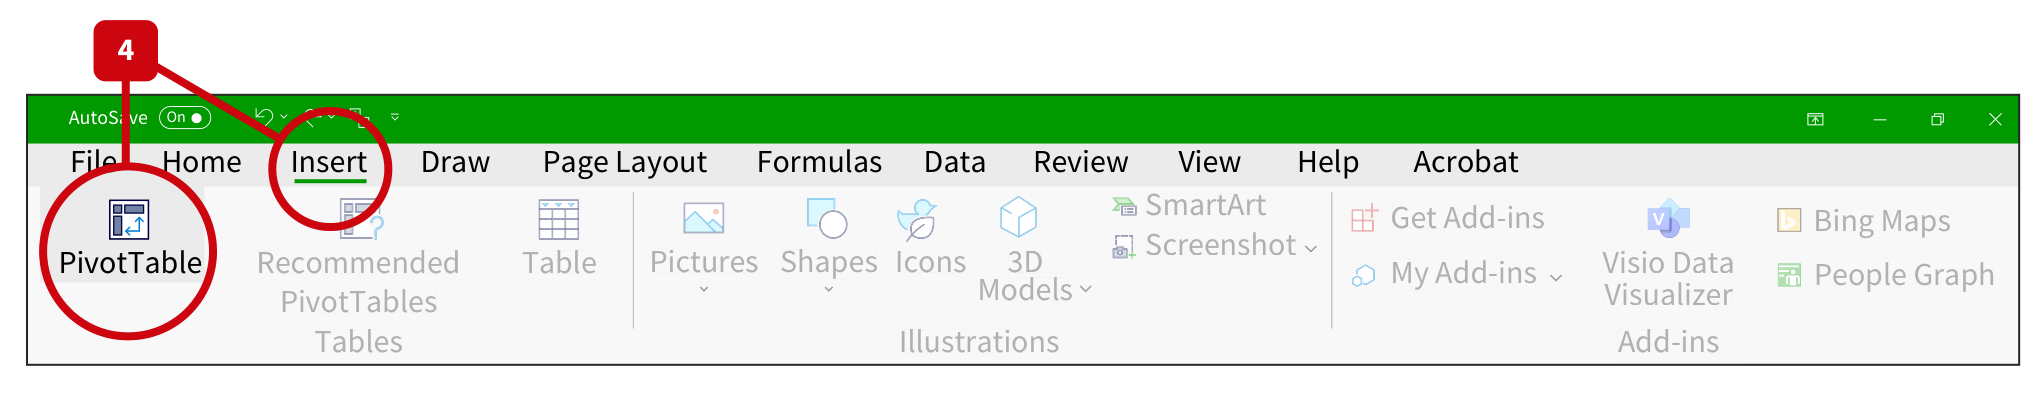
\includegraphics[width=0.95\textwidth,height=0.75\textheight,keepaspectratio]{../textbookForPractice/Figures/Ch_04/ILLUSTRATION 4.32.png}
    \end{figure}
\end{frame}

\begin{frame}{ILLUSTRATION 4.33}
    \begin{figure}[h]
        \centering
        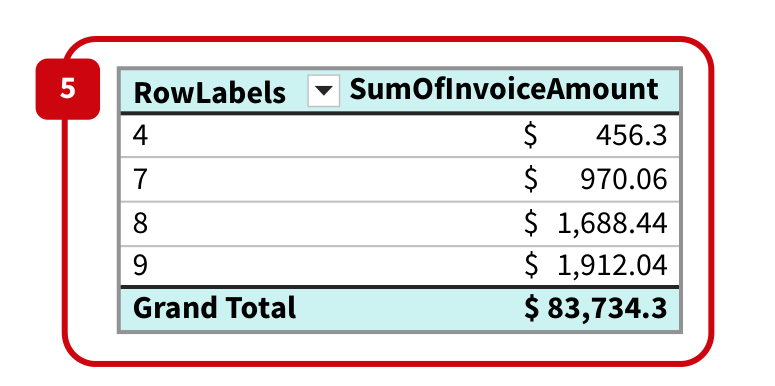
\includegraphics[width=0.95\textwidth,height=0.75\textheight,keepaspectratio]{../textbookForPractice/Figures/Ch_04/ILLUSTRATION 4.33.png}
    \end{figure}
\end{frame}

\begin{frame}{ILLUSTRATION 4.34}
    \begin{figure}[h]
        \centering
        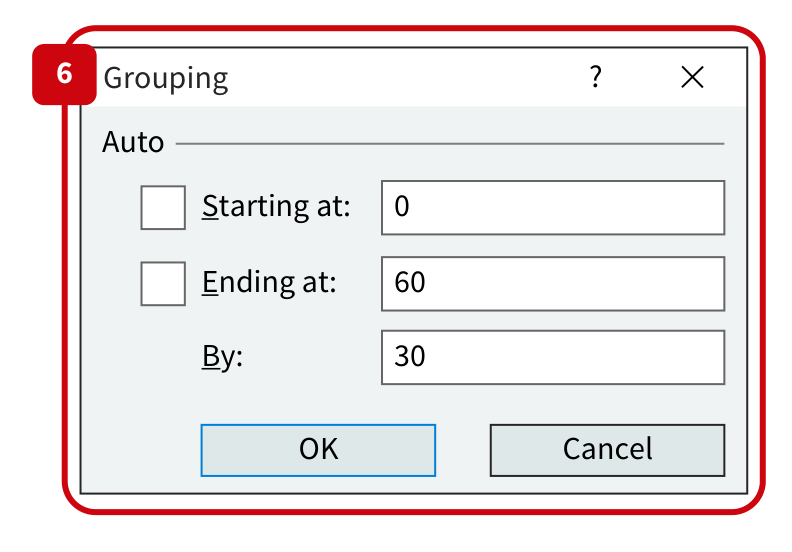
\includegraphics[width=0.95\textwidth,height=0.75\textheight,keepaspectratio]{../textbookForPractice/Figures/Ch_04/ILLUSTRATION 4.34.png}
    \end{figure}
\end{frame}

\begin{frame}{ILLUSTRATION 4.35}
    \begin{figure}[h]
        \centering
        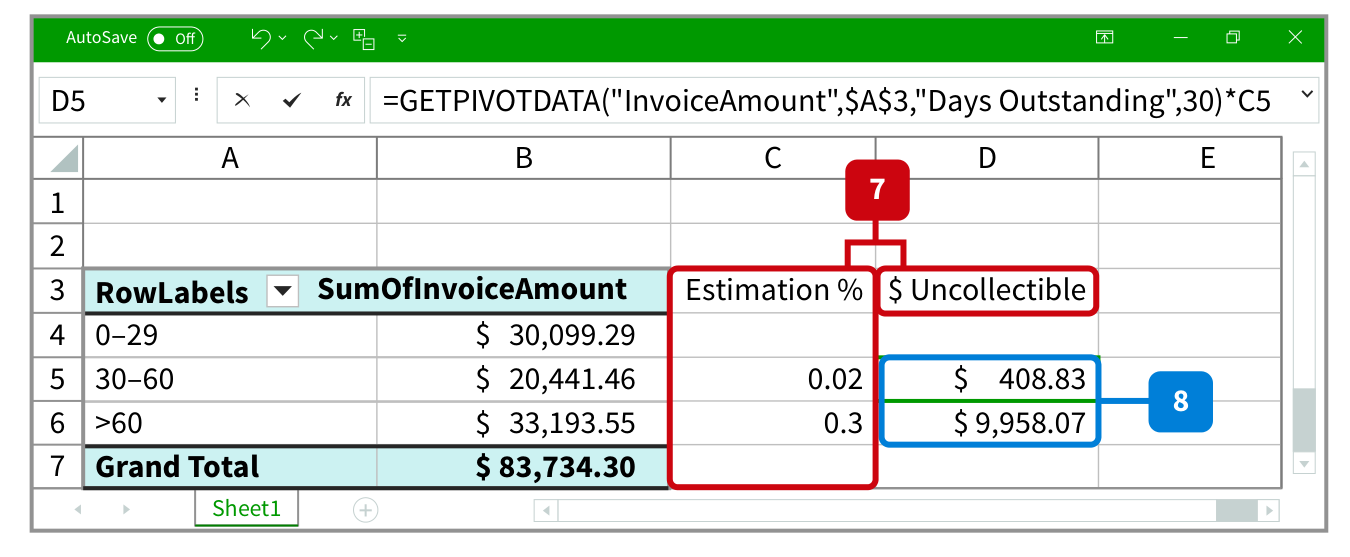
\includegraphics[width=0.95\textwidth,height=0.75\textheight,keepaspectratio]{../textbookForPractice/Figures/Ch_04/ILLUSTRATION 4.35.png}
    \end{figure}
\end{frame}

\begin{frame}{ILLUSTRATION 4.35\_1}
    \begin{figure}[h]
        \centering
        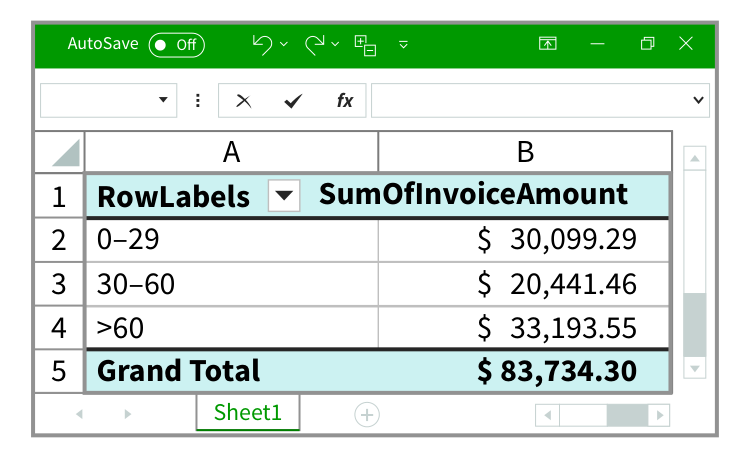
\includegraphics[width=0.95\textwidth,height=0.75\textheight,keepaspectratio]{../textbookForPractice/Figures/Ch_04/ILLUSTRATION 4.35_1.png}
    \end{figure}
\end{frame}

\begin{frame}{ILLUSTRATION 4.36}
    \begin{figure}[h]
        \centering
        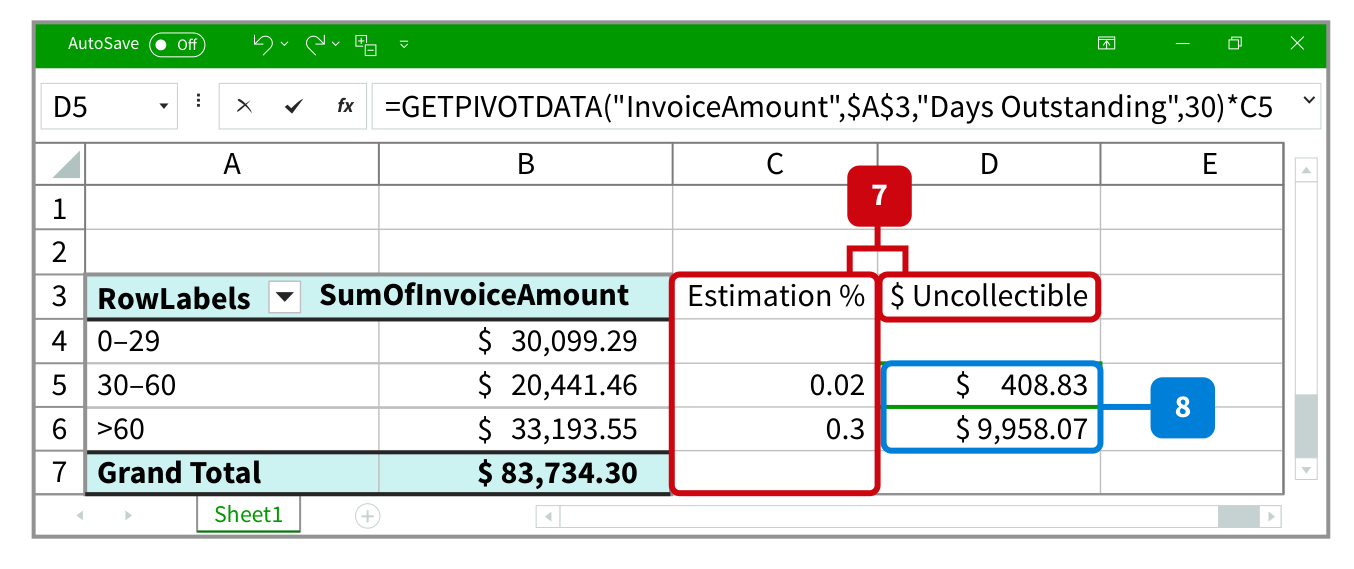
\includegraphics[width=0.95\textwidth,height=0.75\textheight,keepaspectratio]{../textbookForPractice/Figures/Ch_04/ILLUSTRATION 4.36.png}
    \end{figure}
\end{frame}

\begin{frame}{ILLUSTRATION 4.37}
    \begin{figure}[h]
        \centering
        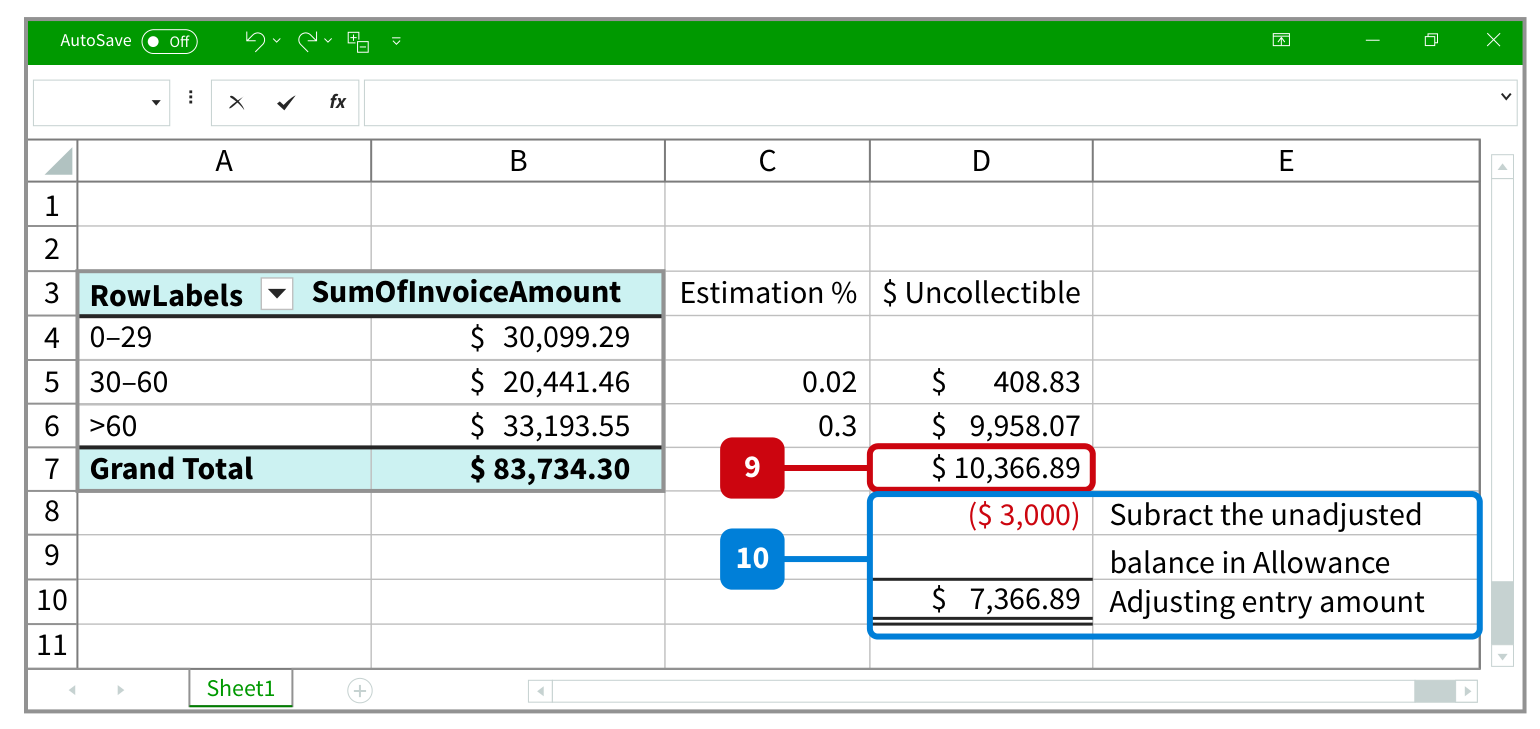
\includegraphics[width=0.95\textwidth,height=0.75\textheight,keepaspectratio]{../textbookForPractice/Figures/Ch_04/ILLUSTRATION 4.37.png}
    \end{figure}
\end{frame}

\begin{frame}{ILLUSTRATION 4.38}
    \begin{figure}[h]
        \centering
        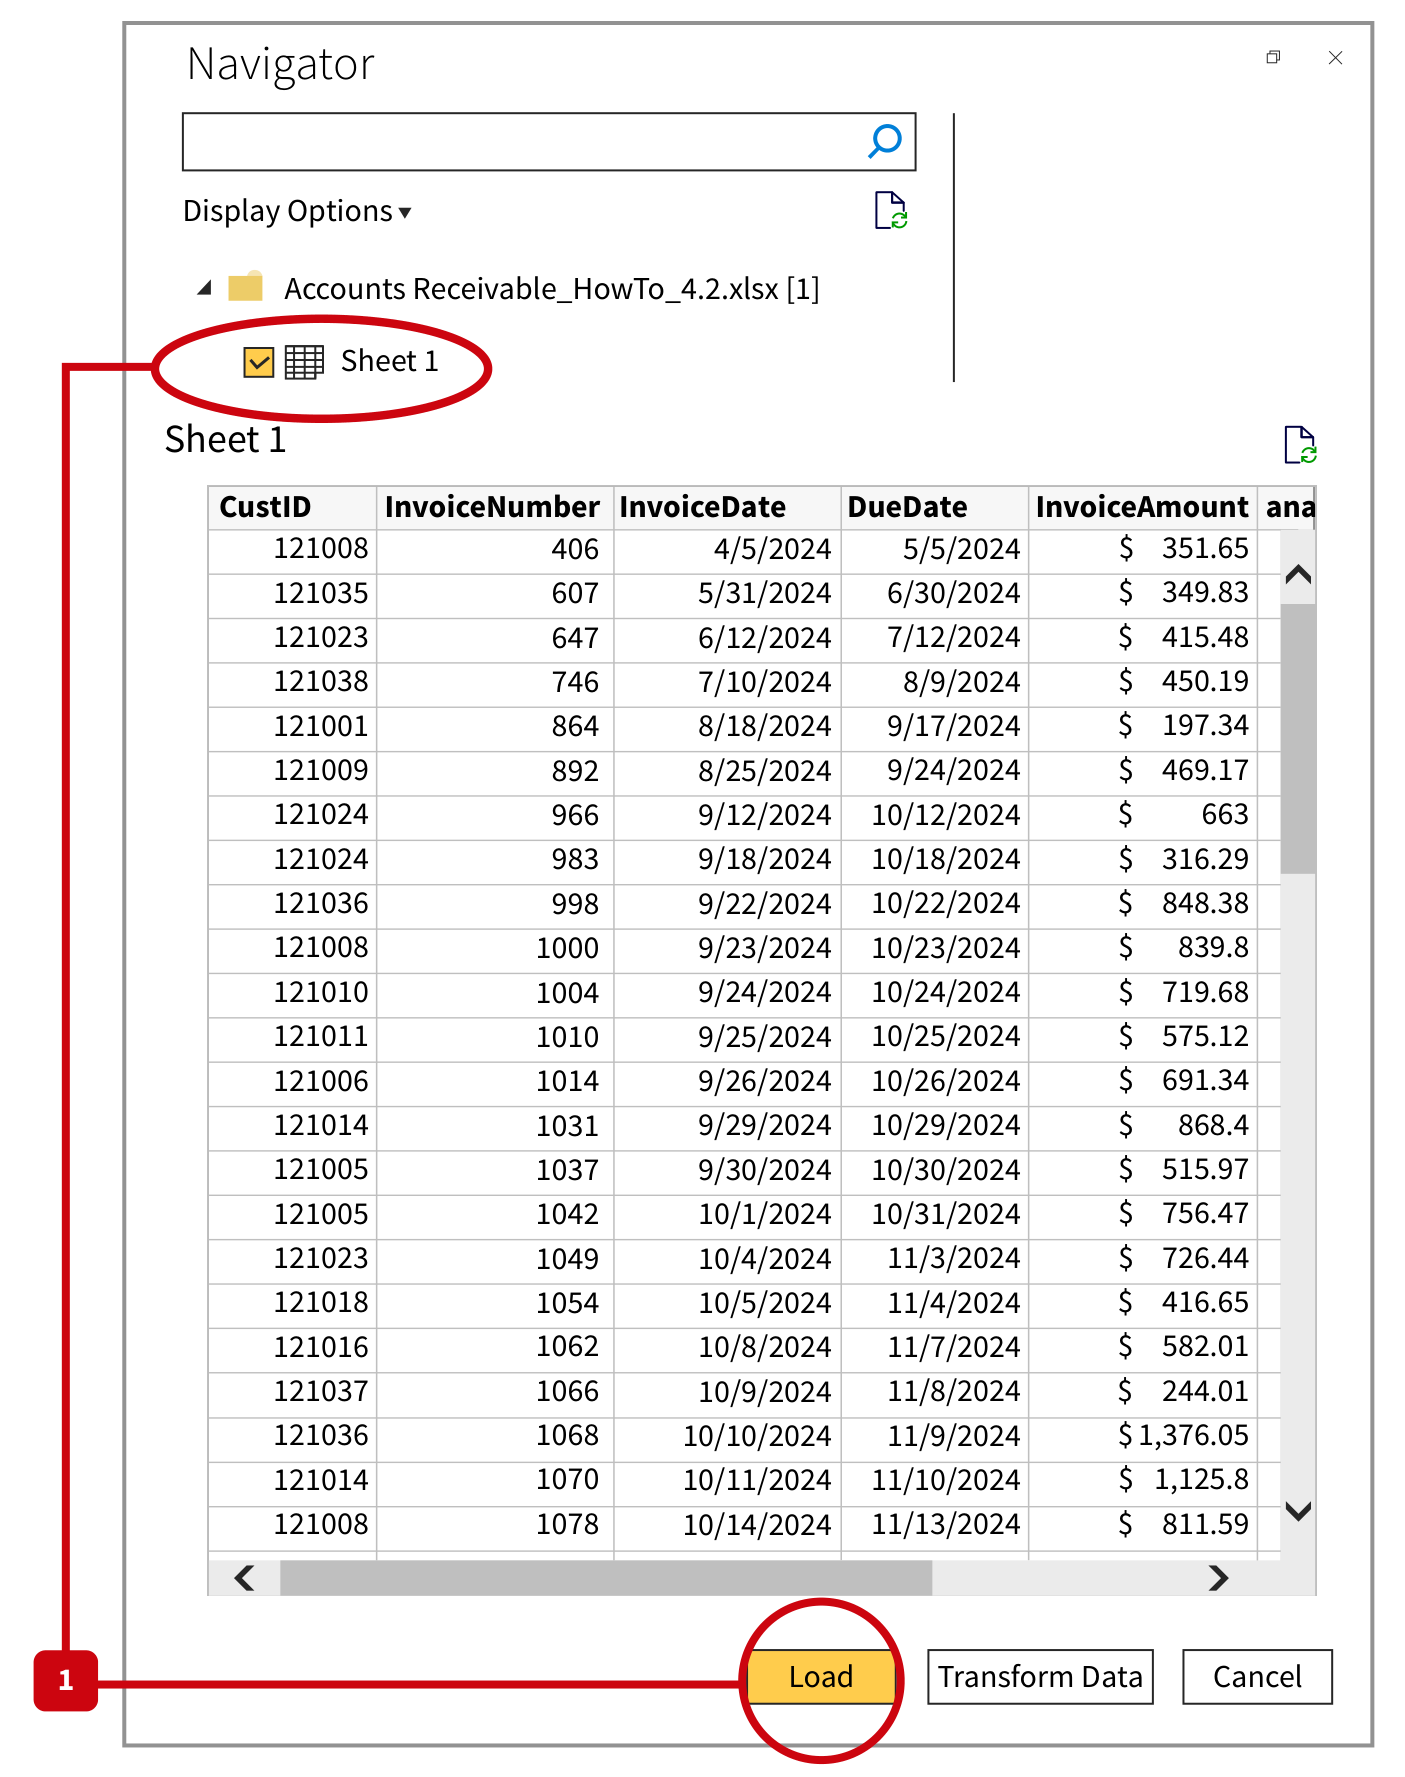
\includegraphics[width=0.95\textwidth,height=0.75\textheight,keepaspectratio]{../textbookForPractice/Figures/Ch_04/ILLUSTRATION 4.38.png}
    \end{figure}
\end{frame}

\begin{frame}{ILLUSTRATION 4.39}
    \begin{figure}[h]
        \centering
        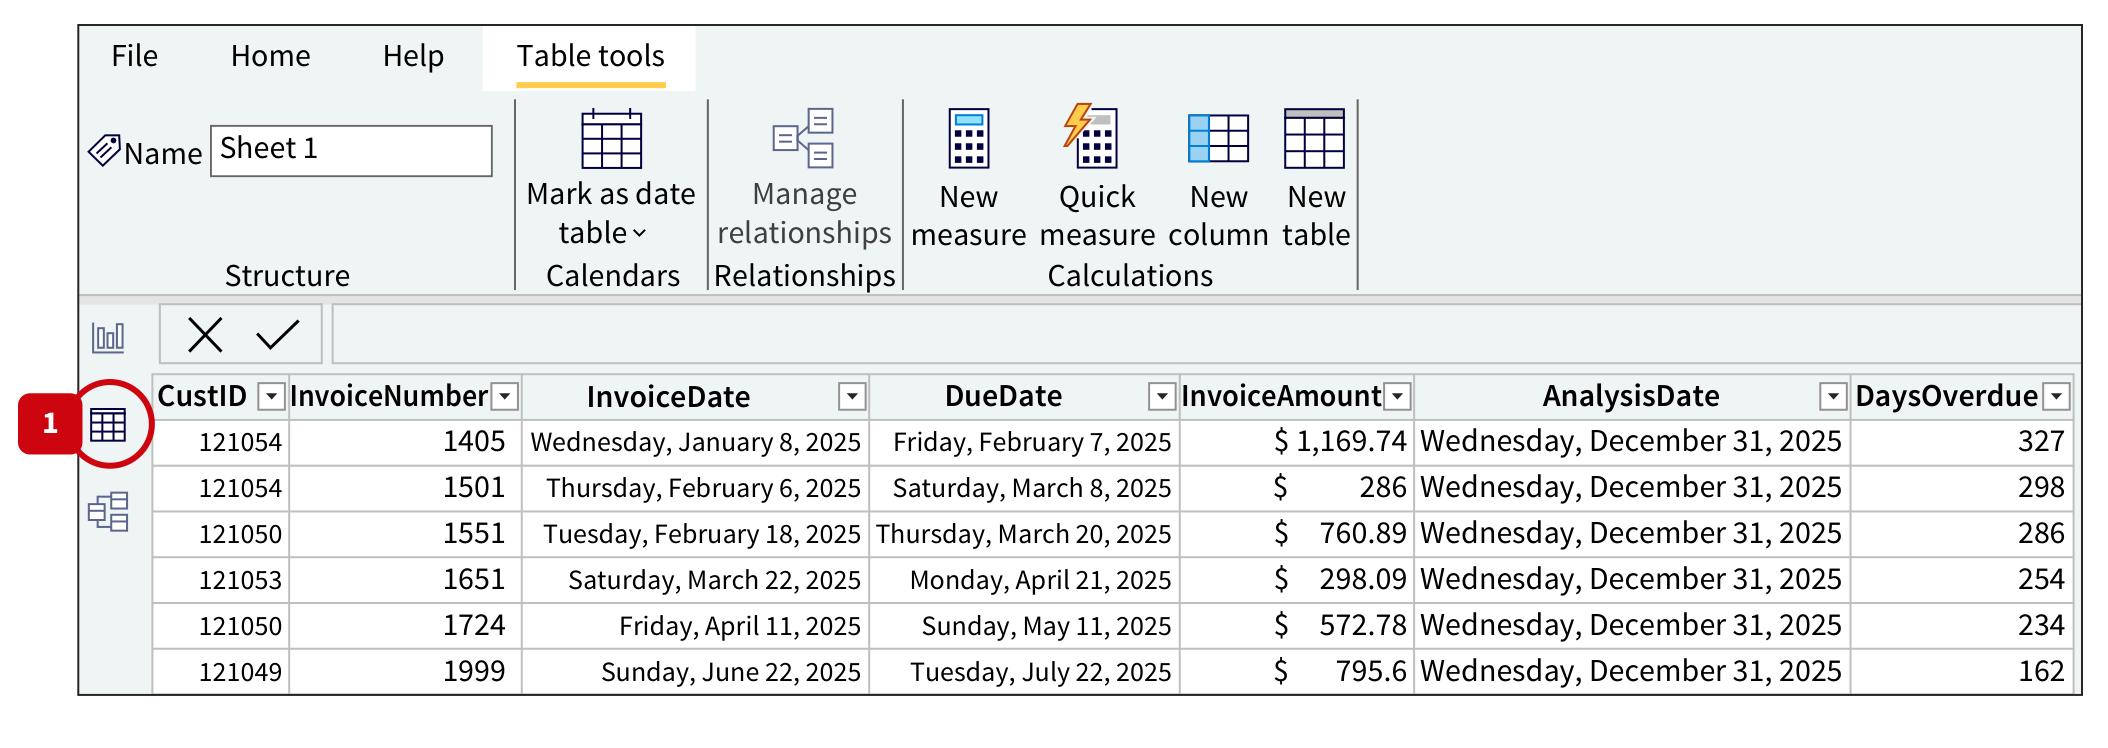
\includegraphics[width=0.95\textwidth,height=0.75\textheight,keepaspectratio]{../textbookForPractice/Figures/Ch_04/ILLUSTRATION 4.39.png}
    \end{figure}
\end{frame}

\begin{frame}{ILLUSTRATION 4.4}
    \begin{figure}[h]
        \centering
        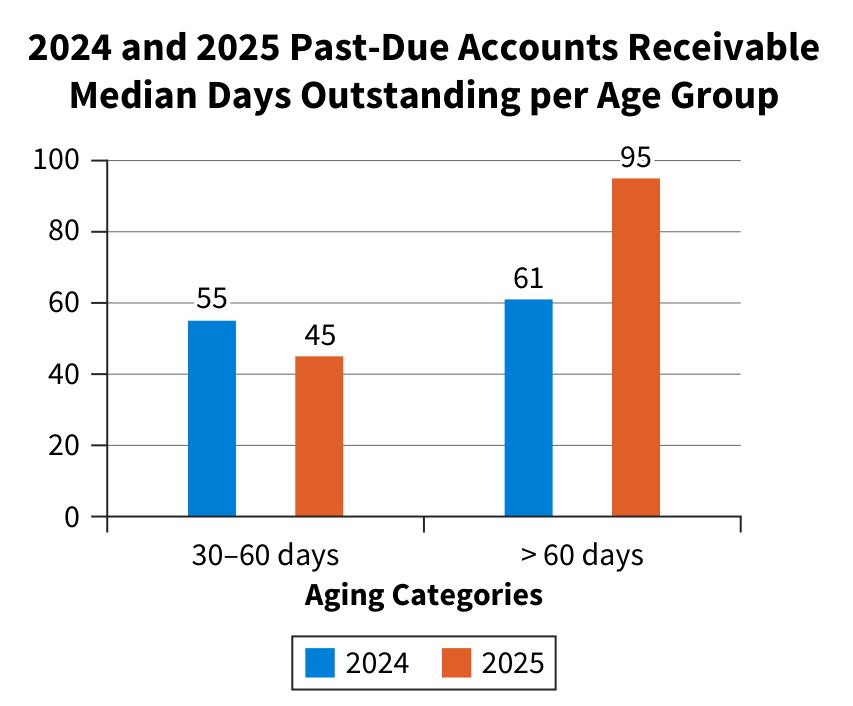
\includegraphics[width=0.95\textwidth,height=0.75\textheight,keepaspectratio]{../textbookForPractice/Figures/Ch_04/ILLUSTRATION 4.4.png}
    \end{figure}
\end{frame}

\begin{frame}{ILLUSTRATION 4.40}
    \begin{figure}[h]
        \centering
        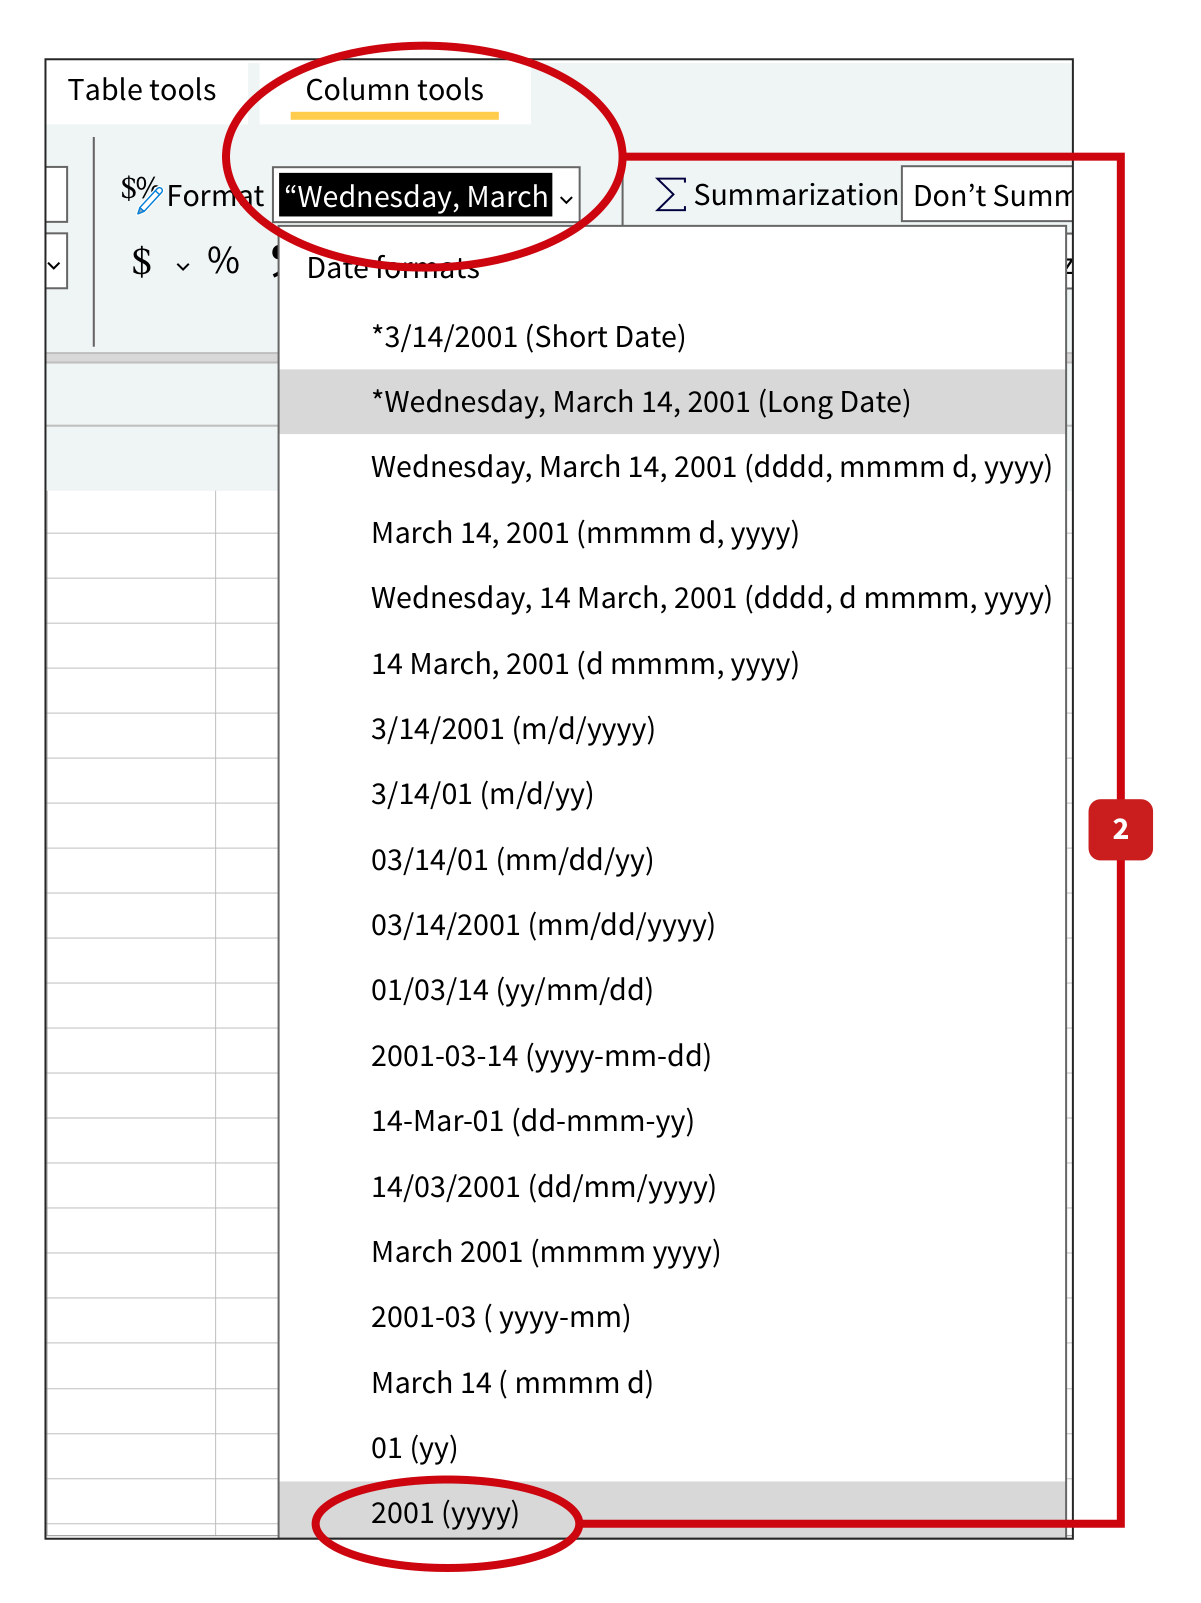
\includegraphics[width=0.95\textwidth,height=0.75\textheight,keepaspectratio]{../textbookForPractice/Figures/Ch_04/ILLUSTRATION 4.40.png}
    \end{figure}
\end{frame}

\begin{frame}{ILLUSTRATION 4.41}
    \begin{figure}[h]
        \centering
        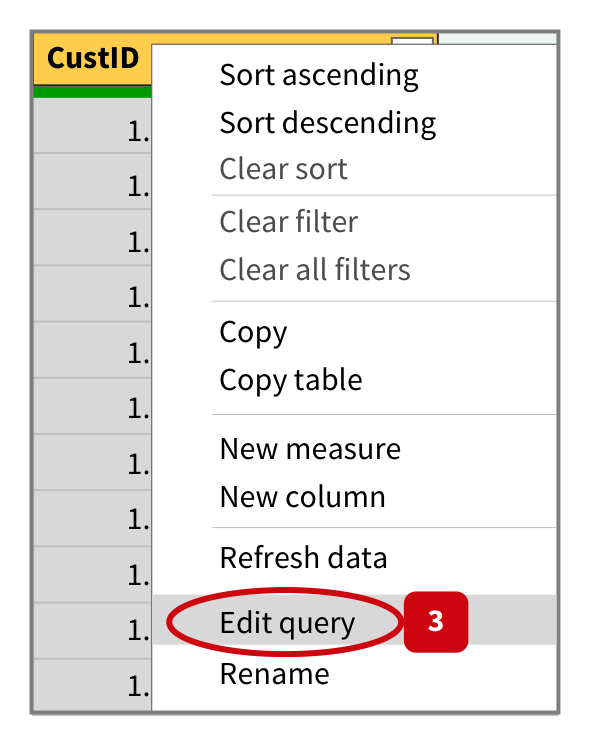
\includegraphics[width=0.95\textwidth,height=0.75\textheight,keepaspectratio]{../textbookForPractice/Figures/Ch_04/ILLUSTRATION 4.41.png}
    \end{figure}
\end{frame}

\begin{frame}{ILLUSTRATION 4.42}
    \begin{figure}[h]
        \centering
        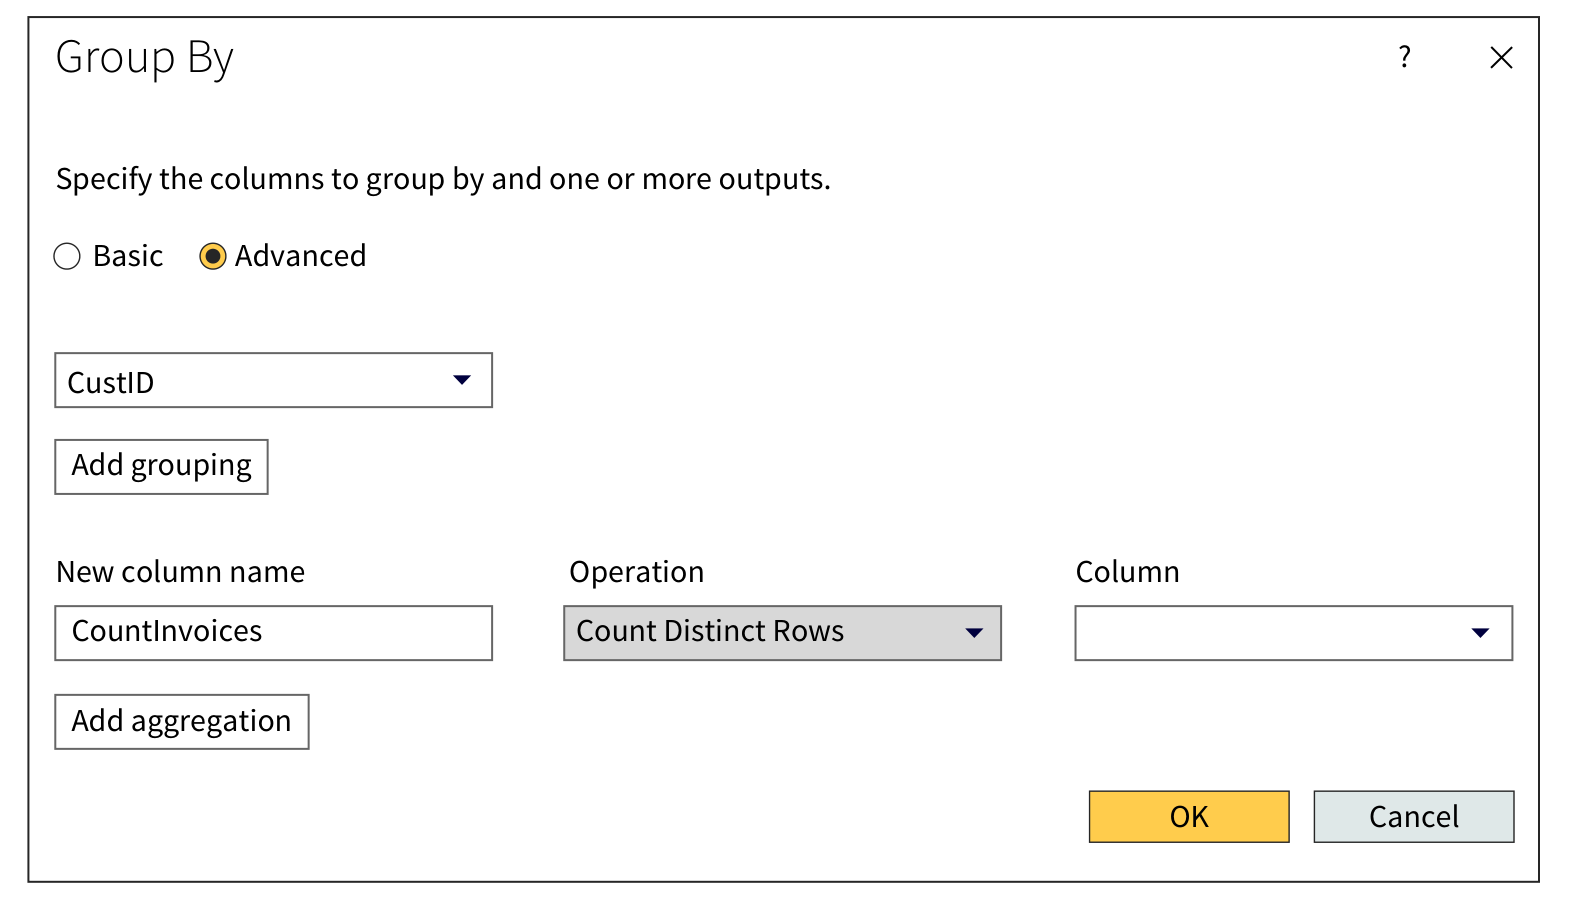
\includegraphics[width=0.95\textwidth,height=0.75\textheight,keepaspectratio]{../textbookForPractice/Figures/Ch_04/ILLUSTRATION 4.42.png}
    \end{figure}
\end{frame}

\begin{frame}{ILLUSTRATION 4.43}
    \begin{figure}[h]
        \centering
        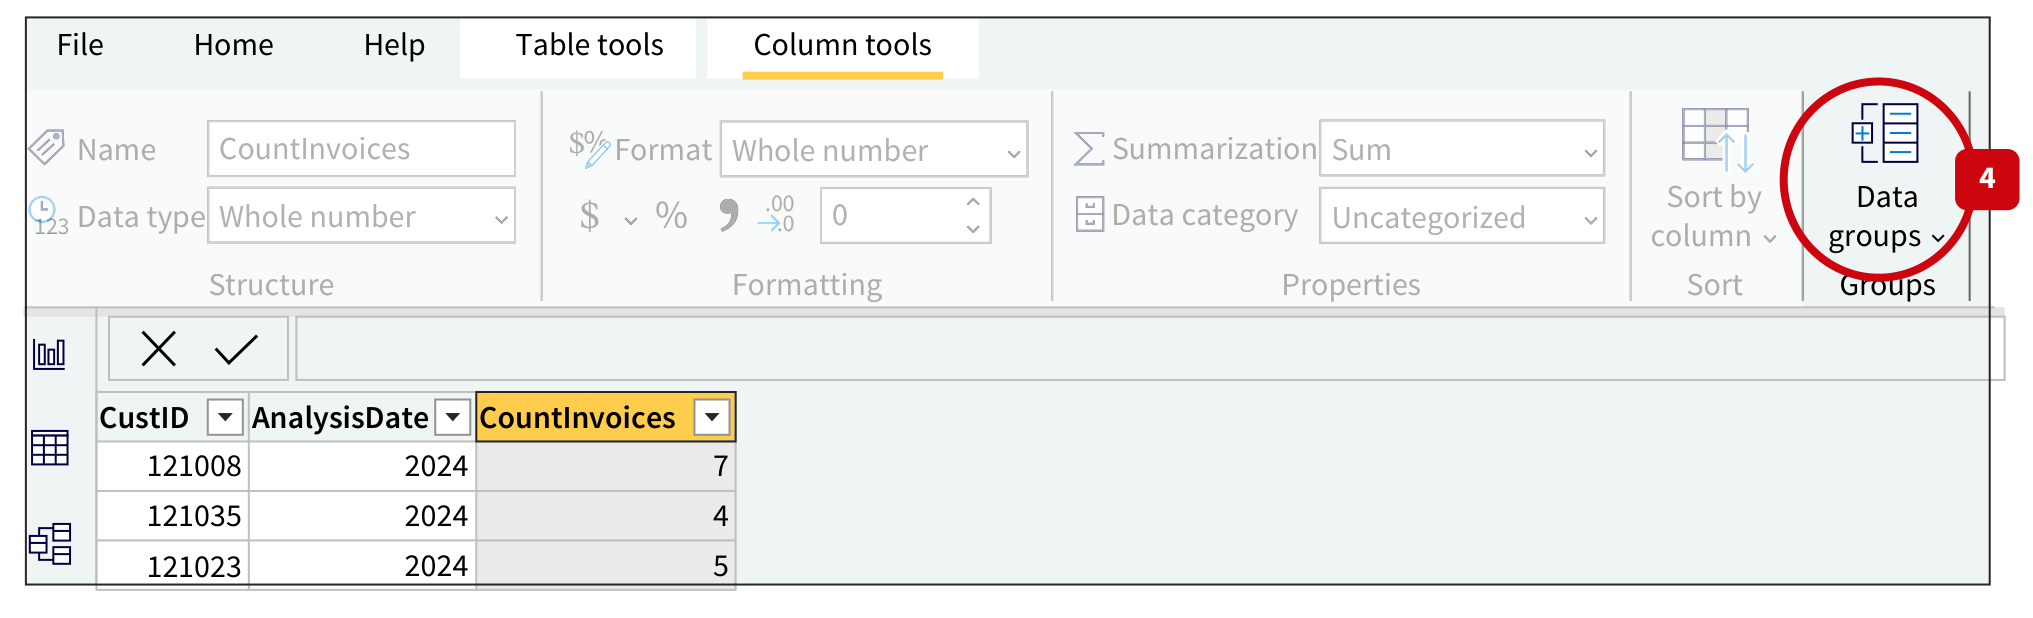
\includegraphics[width=0.95\textwidth,height=0.75\textheight,keepaspectratio]{../textbookForPractice/Figures/Ch_04/ILLUSTRATION 4.43.png}
    \end{figure}
\end{frame}

\begin{frame}{ILLUSTRATION 4.44}
    \begin{figure}[h]
        \centering
        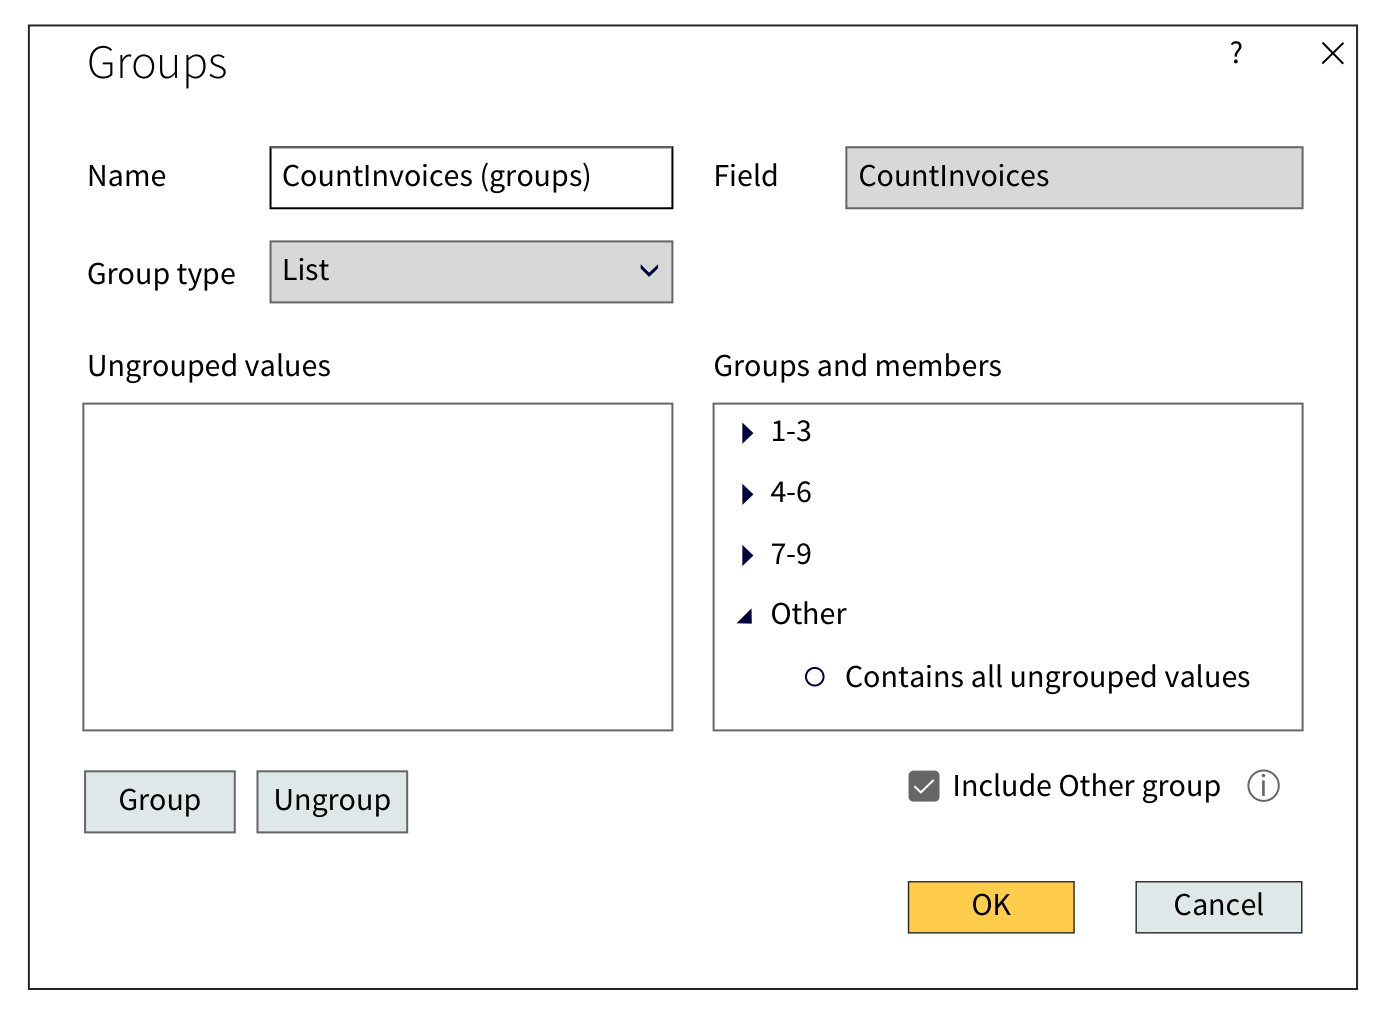
\includegraphics[width=0.95\textwidth,height=0.75\textheight,keepaspectratio]{../textbookForPractice/Figures/Ch_04/ILLUSTRATION 4.44.png}
    \end{figure}
\end{frame}

\begin{frame}{ILLUSTRATION 4.45}
    \begin{figure}[h]
        \centering
        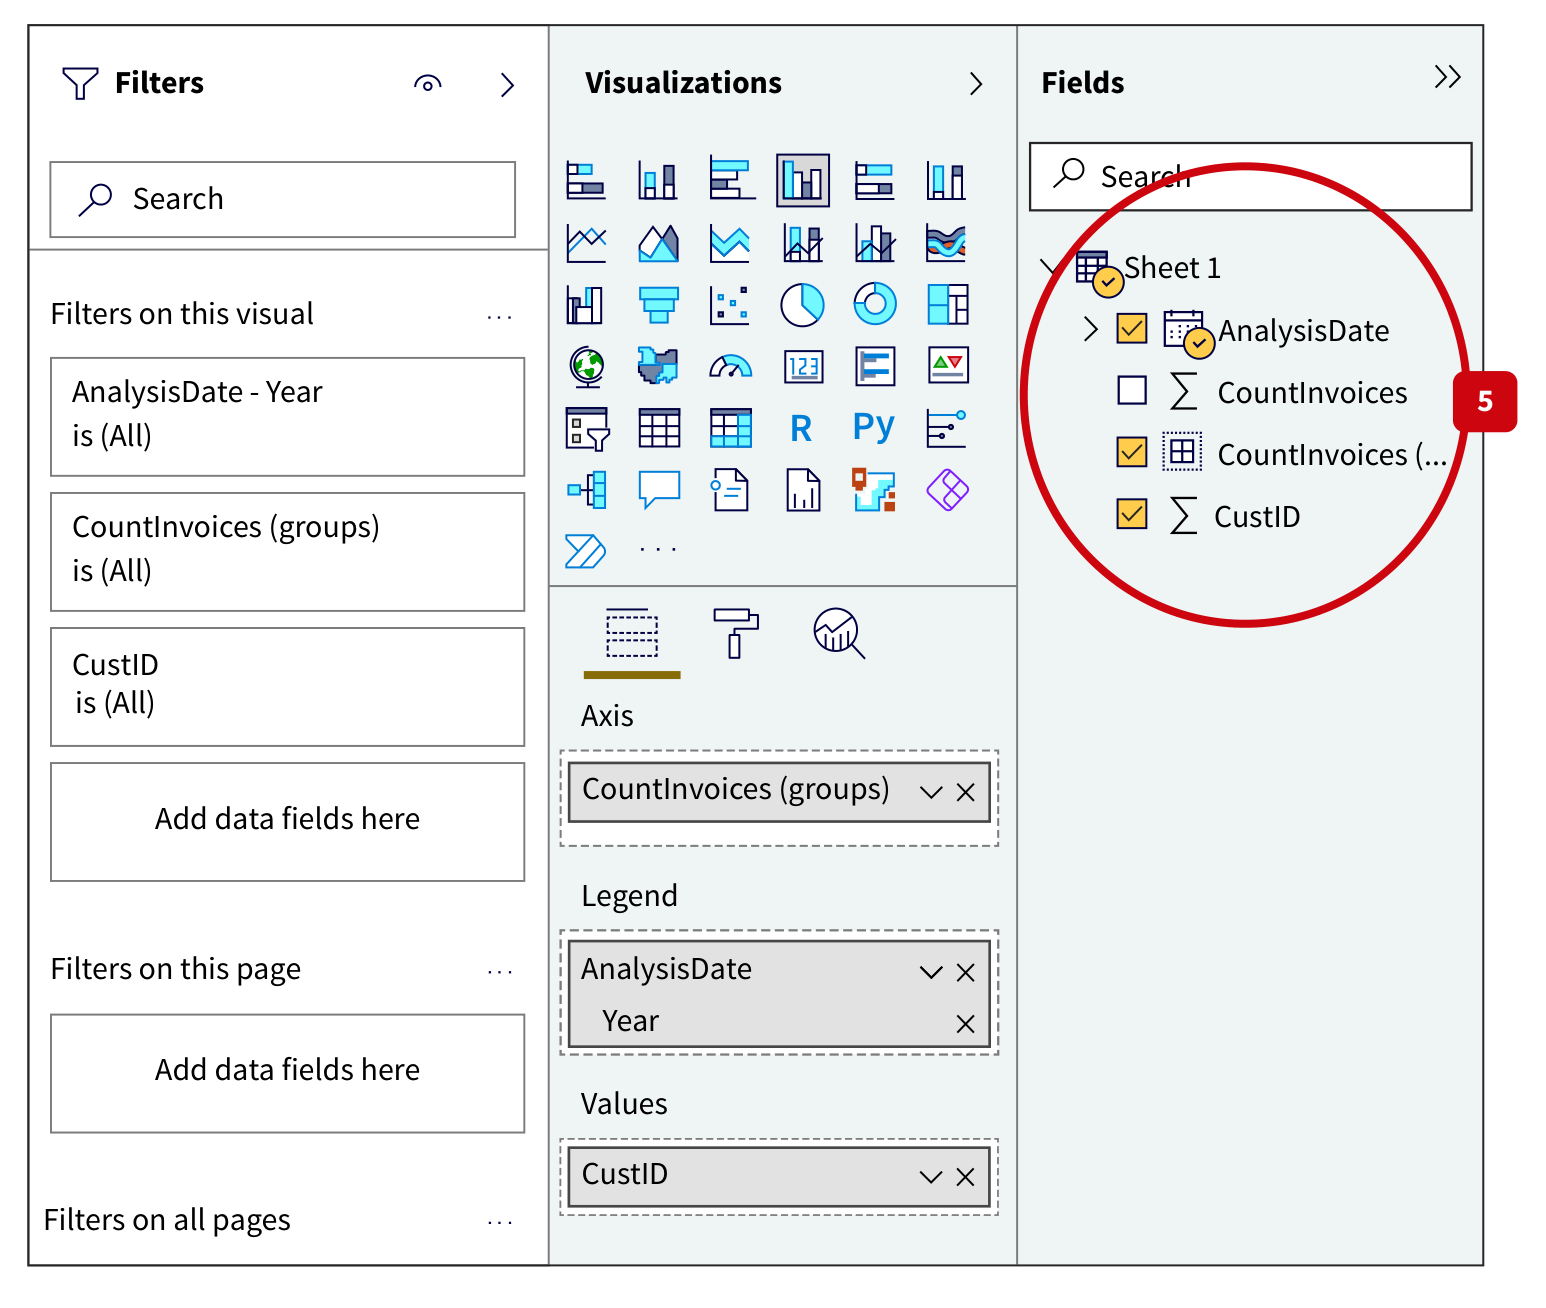
\includegraphics[width=0.95\textwidth,height=0.75\textheight,keepaspectratio]{../textbookForPractice/Figures/Ch_04/ILLUSTRATION 4.45.png}
    \end{figure}
\end{frame}

\begin{frame}{ILLUSTRATION 4.46}
    \begin{figure}[h]
        \centering
        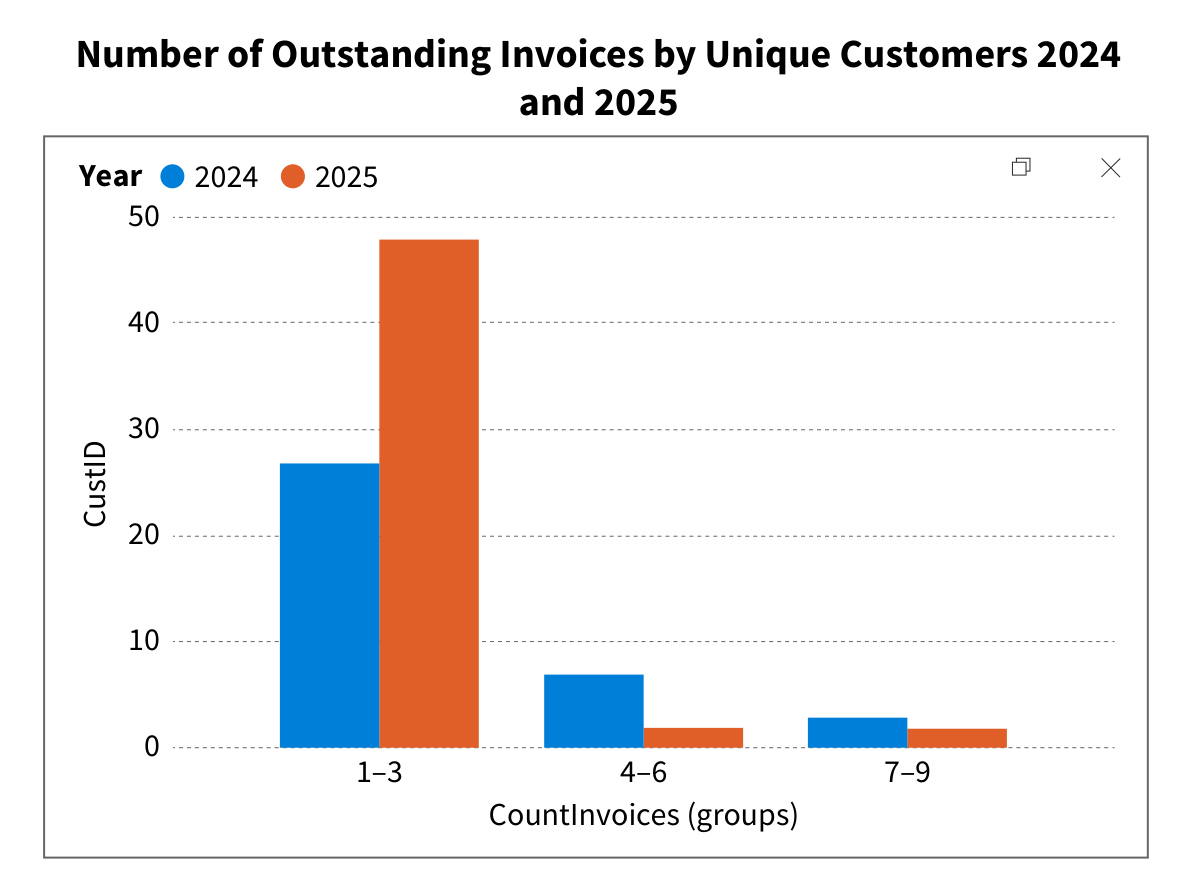
\includegraphics[width=0.95\textwidth,height=0.75\textheight,keepaspectratio]{../textbookForPractice/Figures/Ch_04/ILLUSTRATION 4.46.png}
    \end{figure}
\end{frame}

\begin{frame}{ILLUSTRATION 4.5}
    \begin{figure}[h]
        \centering
        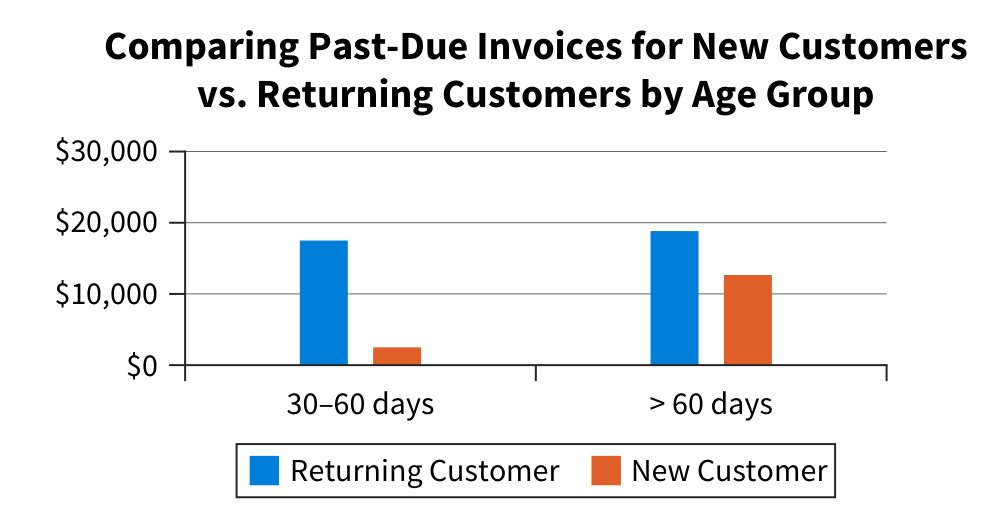
\includegraphics[width=0.95\textwidth,height=0.75\textheight,keepaspectratio]{../textbookForPractice/Figures/Ch_04/ILLUSTRATION 4.5.png}
    \end{figure}
\end{frame}

\begin{frame}{ILLUSTRATION 4.6}
    \begin{figure}[h]
        \centering
        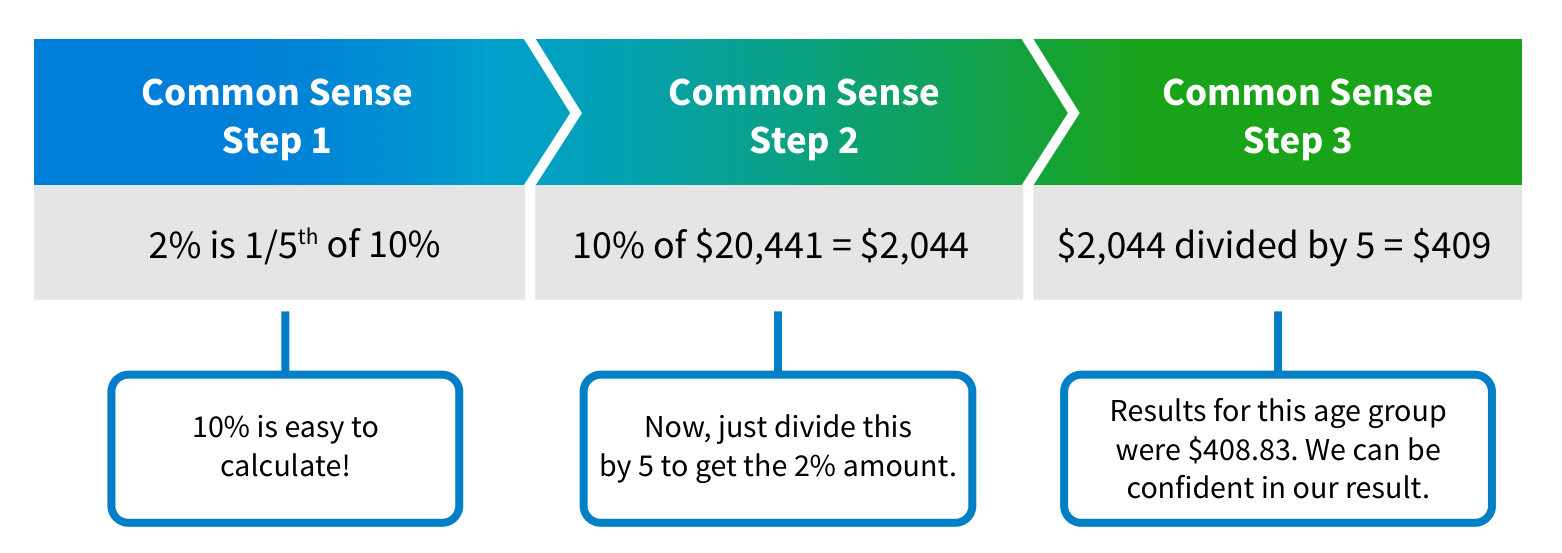
\includegraphics[width=0.95\textwidth,height=0.75\textheight,keepaspectratio]{../textbookForPractice/Figures/Ch_04/ILLUSTRATION 4.6.png}
    \end{figure}
\end{frame}

\begin{frame}{ILLUSTRATION 4.7}
    \begin{figure}[h]
        \centering
        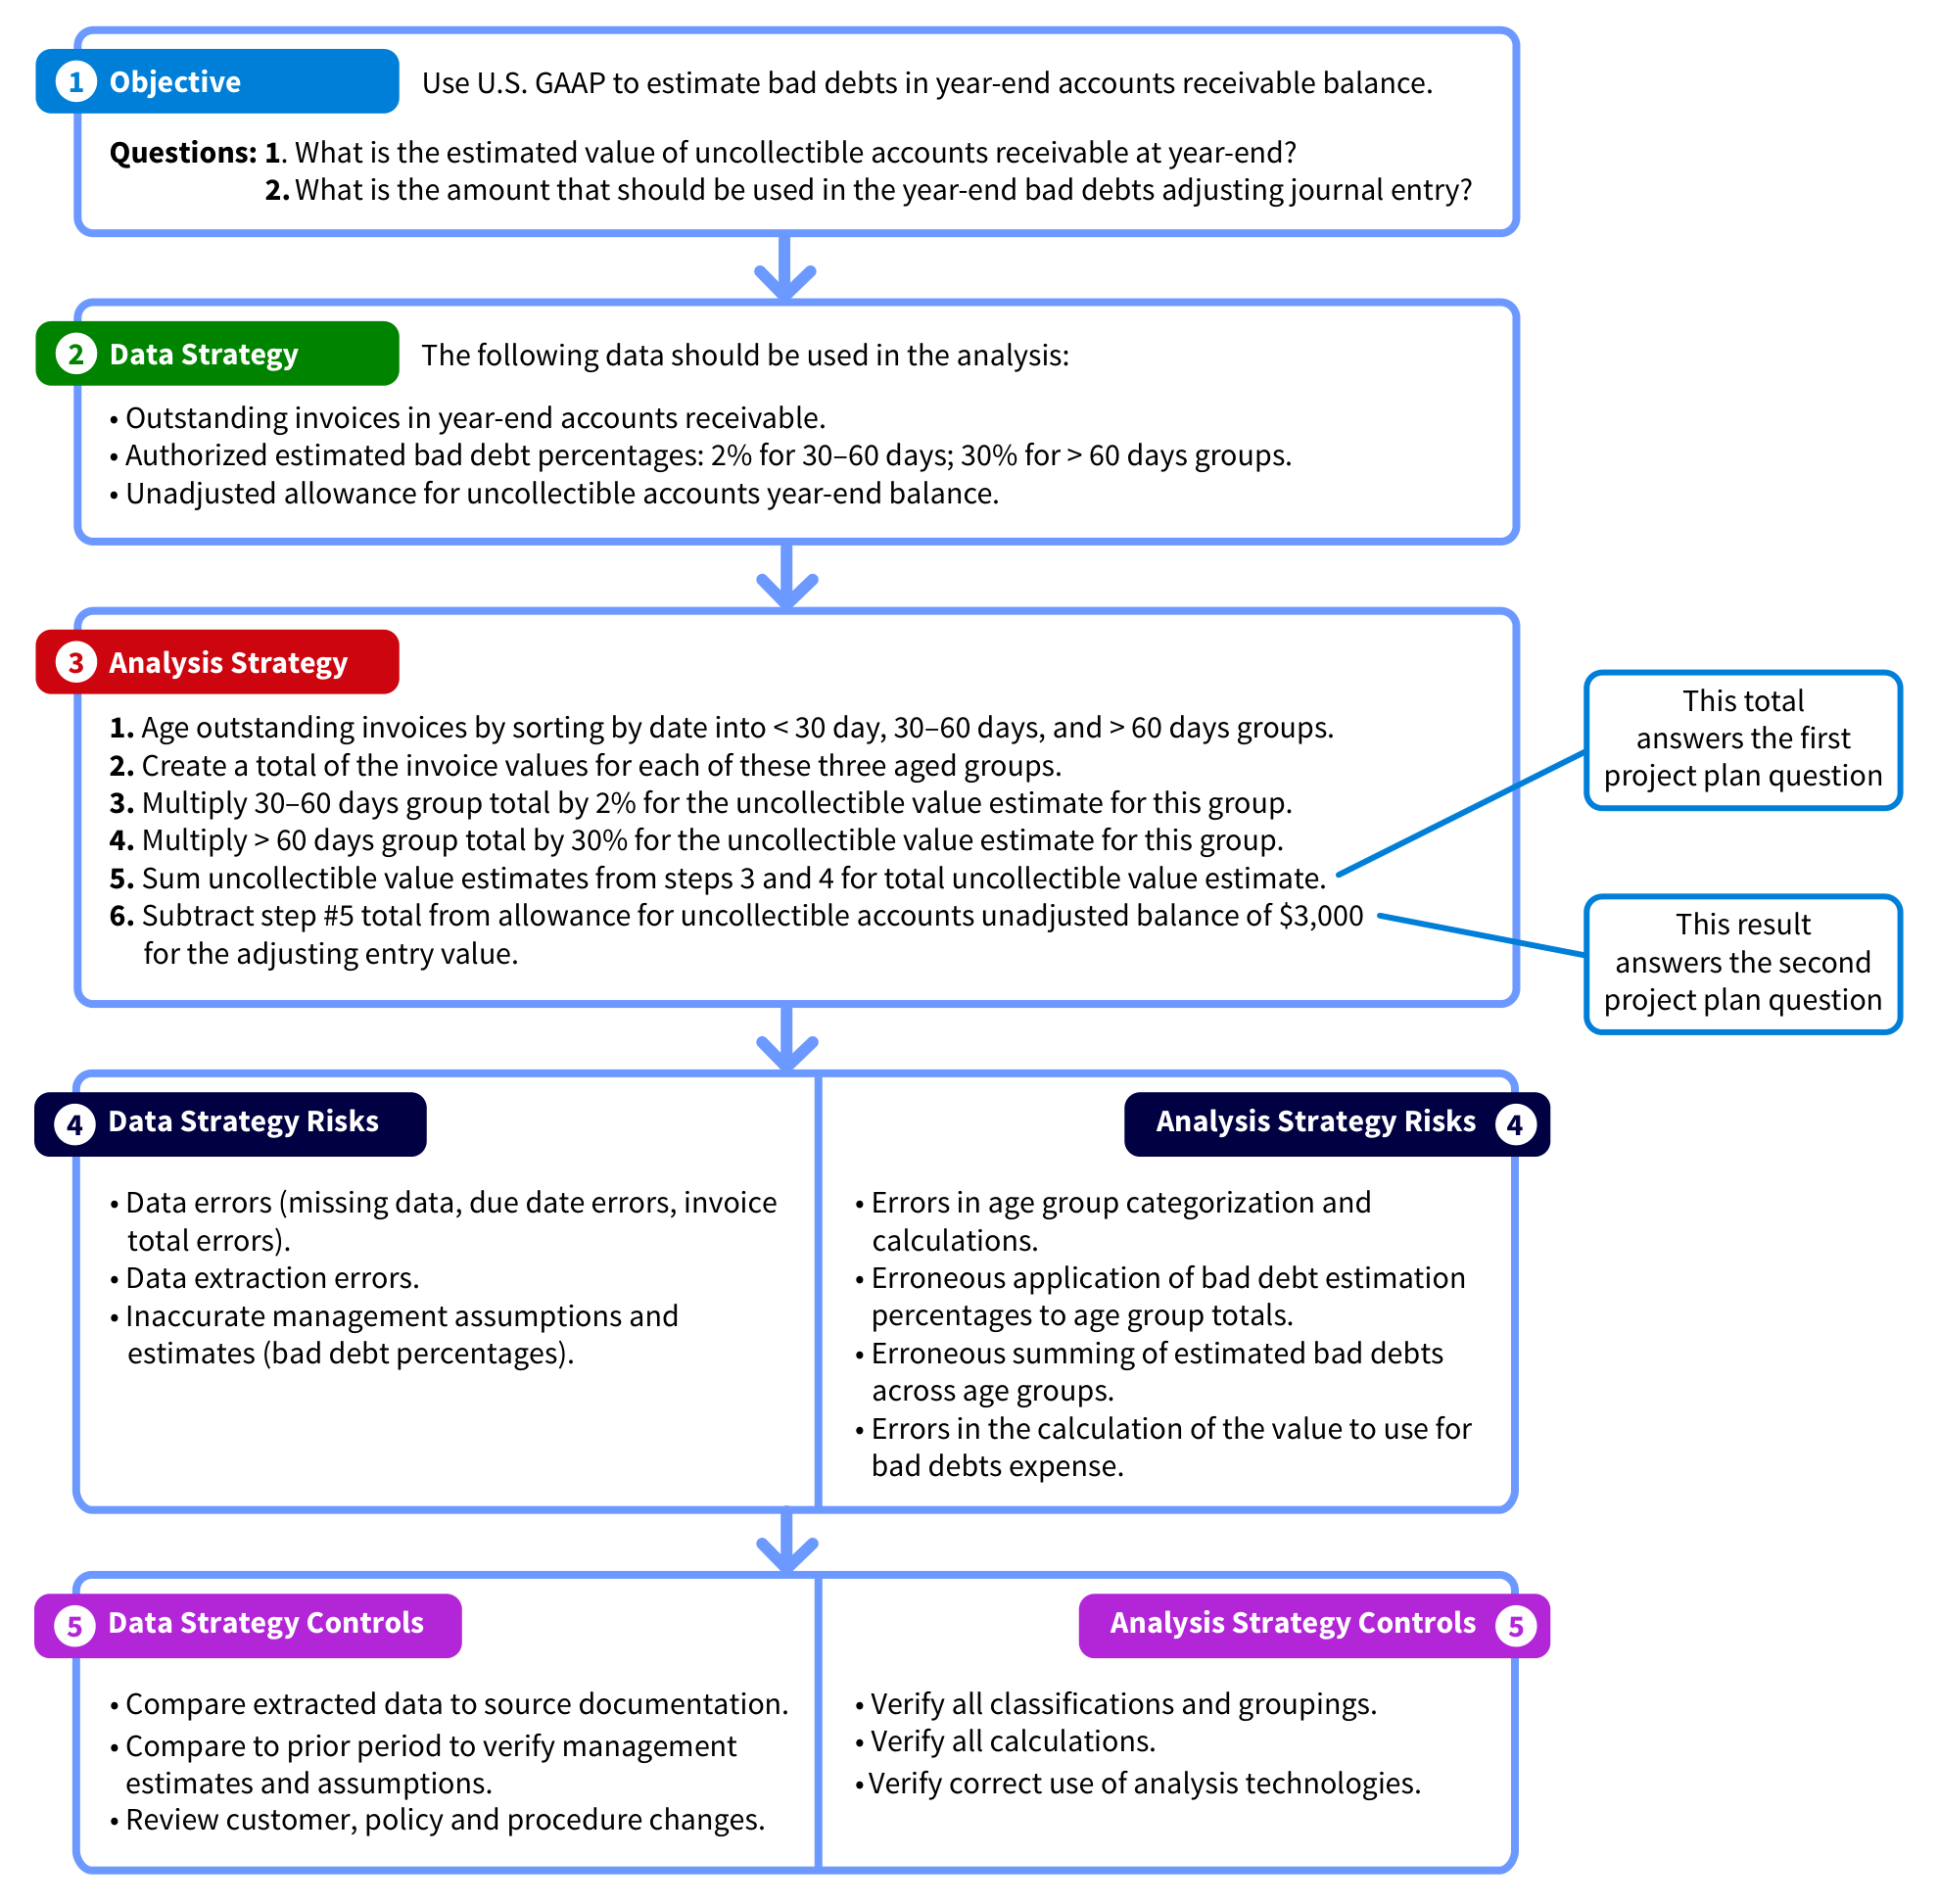
\includegraphics[width=0.95\textwidth,height=0.75\textheight,keepaspectratio]{../textbookForPractice/Figures/Ch_04/ILLUSTRATION 4.7.png}
    \end{figure}
\end{frame}

\begin{frame}{ILLUSTRATION 4.8}
    \begin{figure}[h]
        \centering
        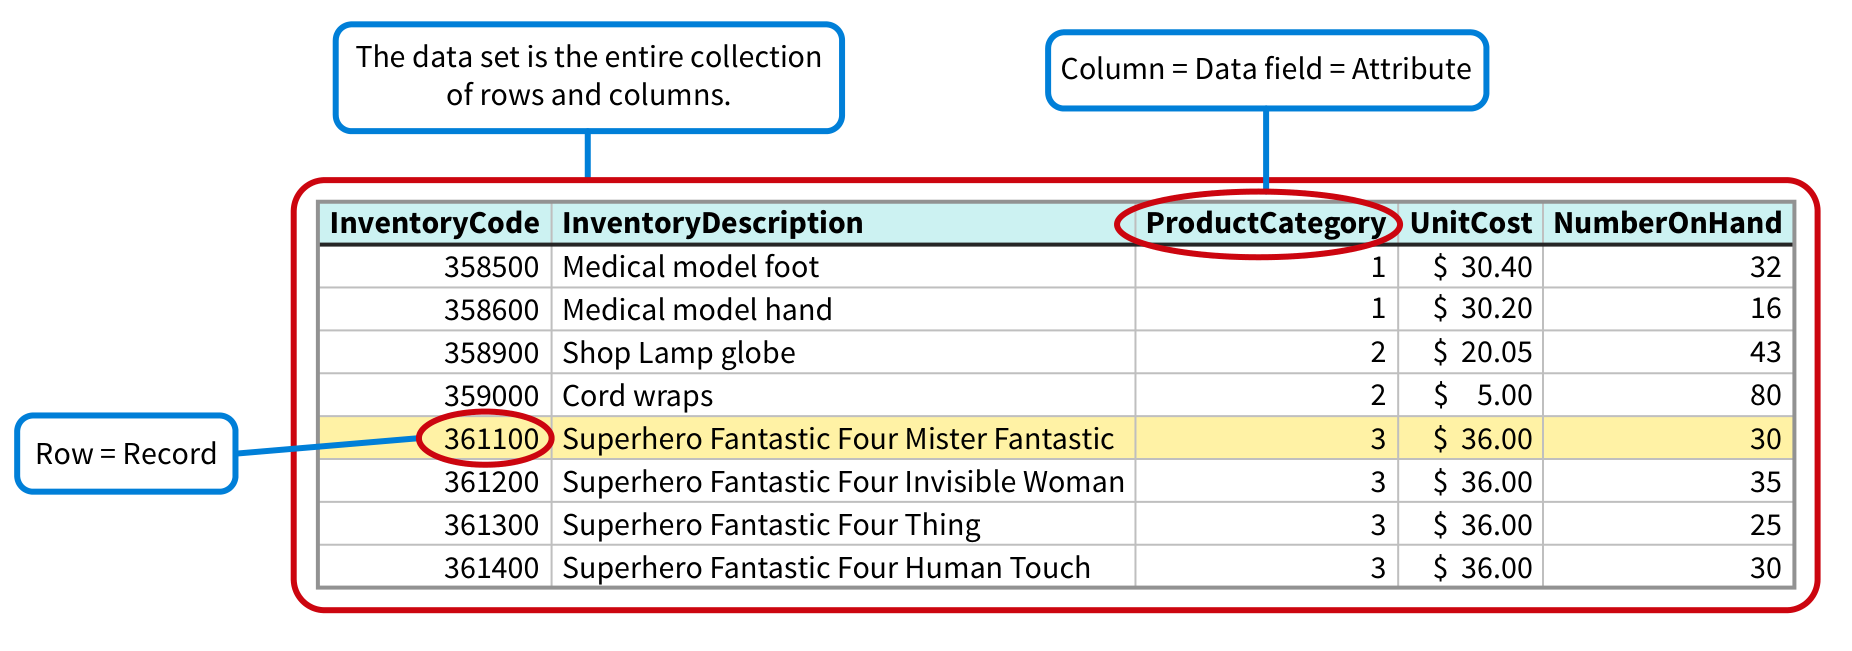
\includegraphics[width=0.95\textwidth,height=0.75\textheight,keepaspectratio]{../textbookForPractice/Figures/Ch_04/ILLUSTRATION 4.8.png}
    \end{figure}
\end{frame}

\begin{frame}{ILLUSTRATION 4.9}
    \begin{figure}[h]
        \centering
        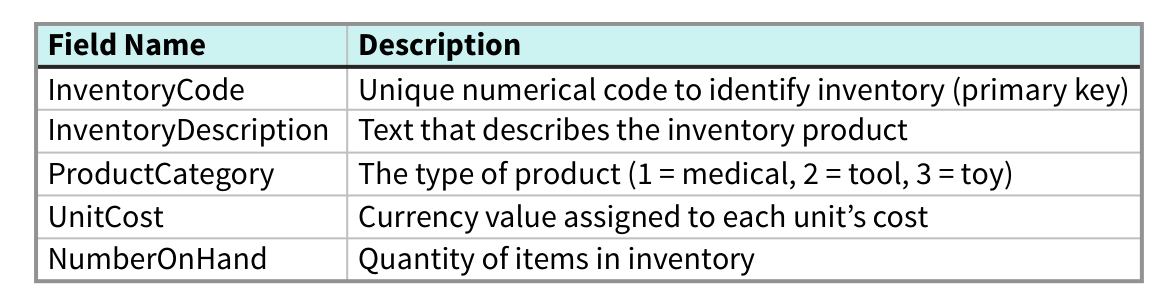
\includegraphics[width=0.95\textwidth,height=0.75\textheight,keepaspectratio]{../textbookForPractice/Figures/Ch_04/ILLUSTRATION 4.9.png}
    \end{figure}
\end{frame}

\begin{frame}{Info 04.2}
    \begin{figure}[h]
        \centering
        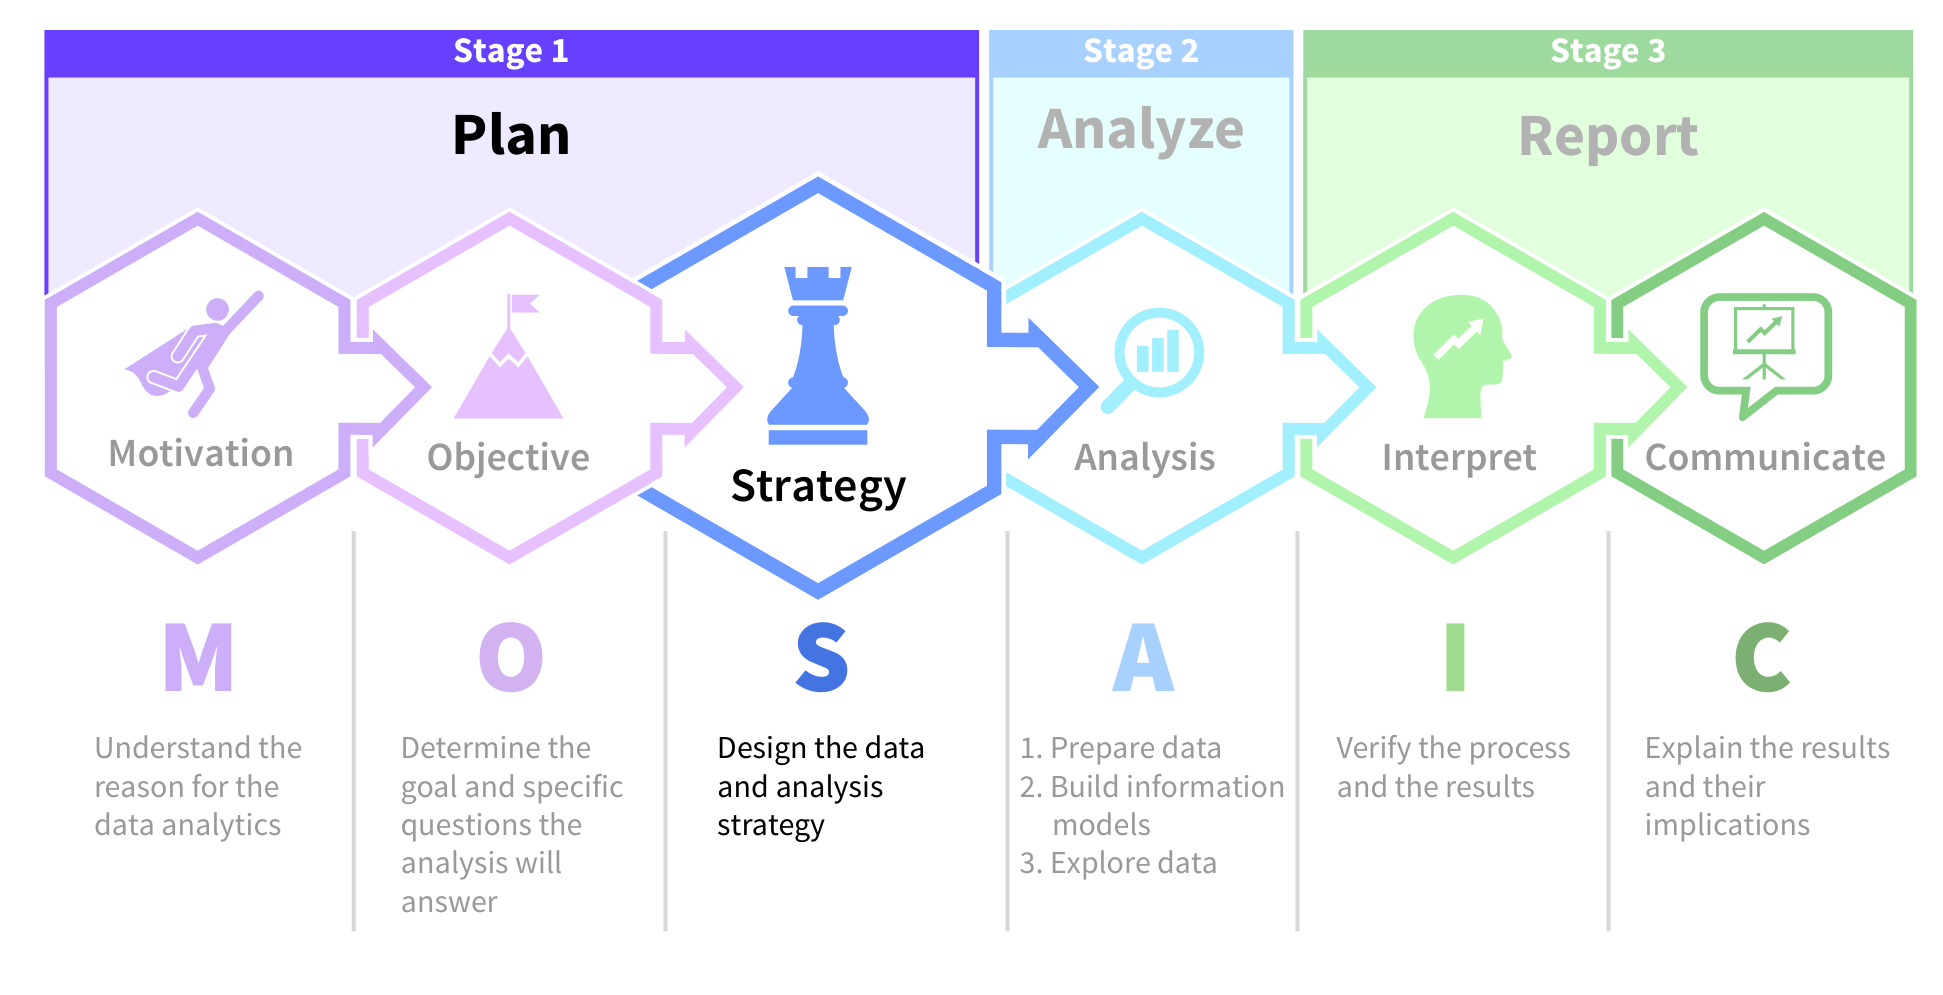
\includegraphics[width=0.95\textwidth,height=0.75\textheight,keepaspectratio]{../textbookForPractice/Figures/Ch_04/Info 04.2.png}
    \end{figure}
\end{frame}

\begin{frame}{Kết thúc}
    \begin{center}
        \Huge \textbf{Hỏi \& Đáp} \\
        \vspace{1cm}
        \Large Cảm ơn các bạn đã lắng nghe!
    \end{center}
\end{frame}

\end{document}
